%%%%%%%%%%%%%%%%%%%%%%%%%%%%%%%%%%%%%%
% A presentation by Gilles Bertrand  %
% gilles.bertrand at ieee dot org   %
% December 2006            %
%%%%%%%%%%%%%%%%%%%%%%%%%%%%%%%%%%%%%%

\documentclass[pdf]{beamer}
\usetheme{Antibes}

\usepackage{time}       % date and time
\usepackage{graphicx}
\usepackage[T1]{fontenc}    % european characters
%\usepackage{courier}
\usepackage{amssymb,amsmath}  % use mathematical symbols
\usepackage{palatino}                  % use palatino as the default font
\setbeamercovered{transparent}

\begin{document}

% here you define the information that will be displayed in the title/cover page
\title[Lego Racing Team]{Lego Racing Team\\\small{Midterm presentation}}
%\subtitle {subtitle}
\author[...]{Christian Dietz, Jan Seeger, Julian Tratsch, Rainer Sch\"{o}nberger, Wenwen Chen\\}
\date{10. Juni 2013}

% this is used in the pdf information
\subject{Midterm presentation}

% here you build the title page
\frame{
 \titlepage
}

% outline
%\AtBeginSection[]
%{
% \begin{frame}
%  \frametitle{Kapitel\"{u}bersicht}
%  \small
%  \tableofcontents[currentsection,hideothersubsections]
%  \normalsize
% \end{frame}
%}


\section{Motivation}
\subsection{Lego -> Problem}
\begin{frame}
  \begin{center}
  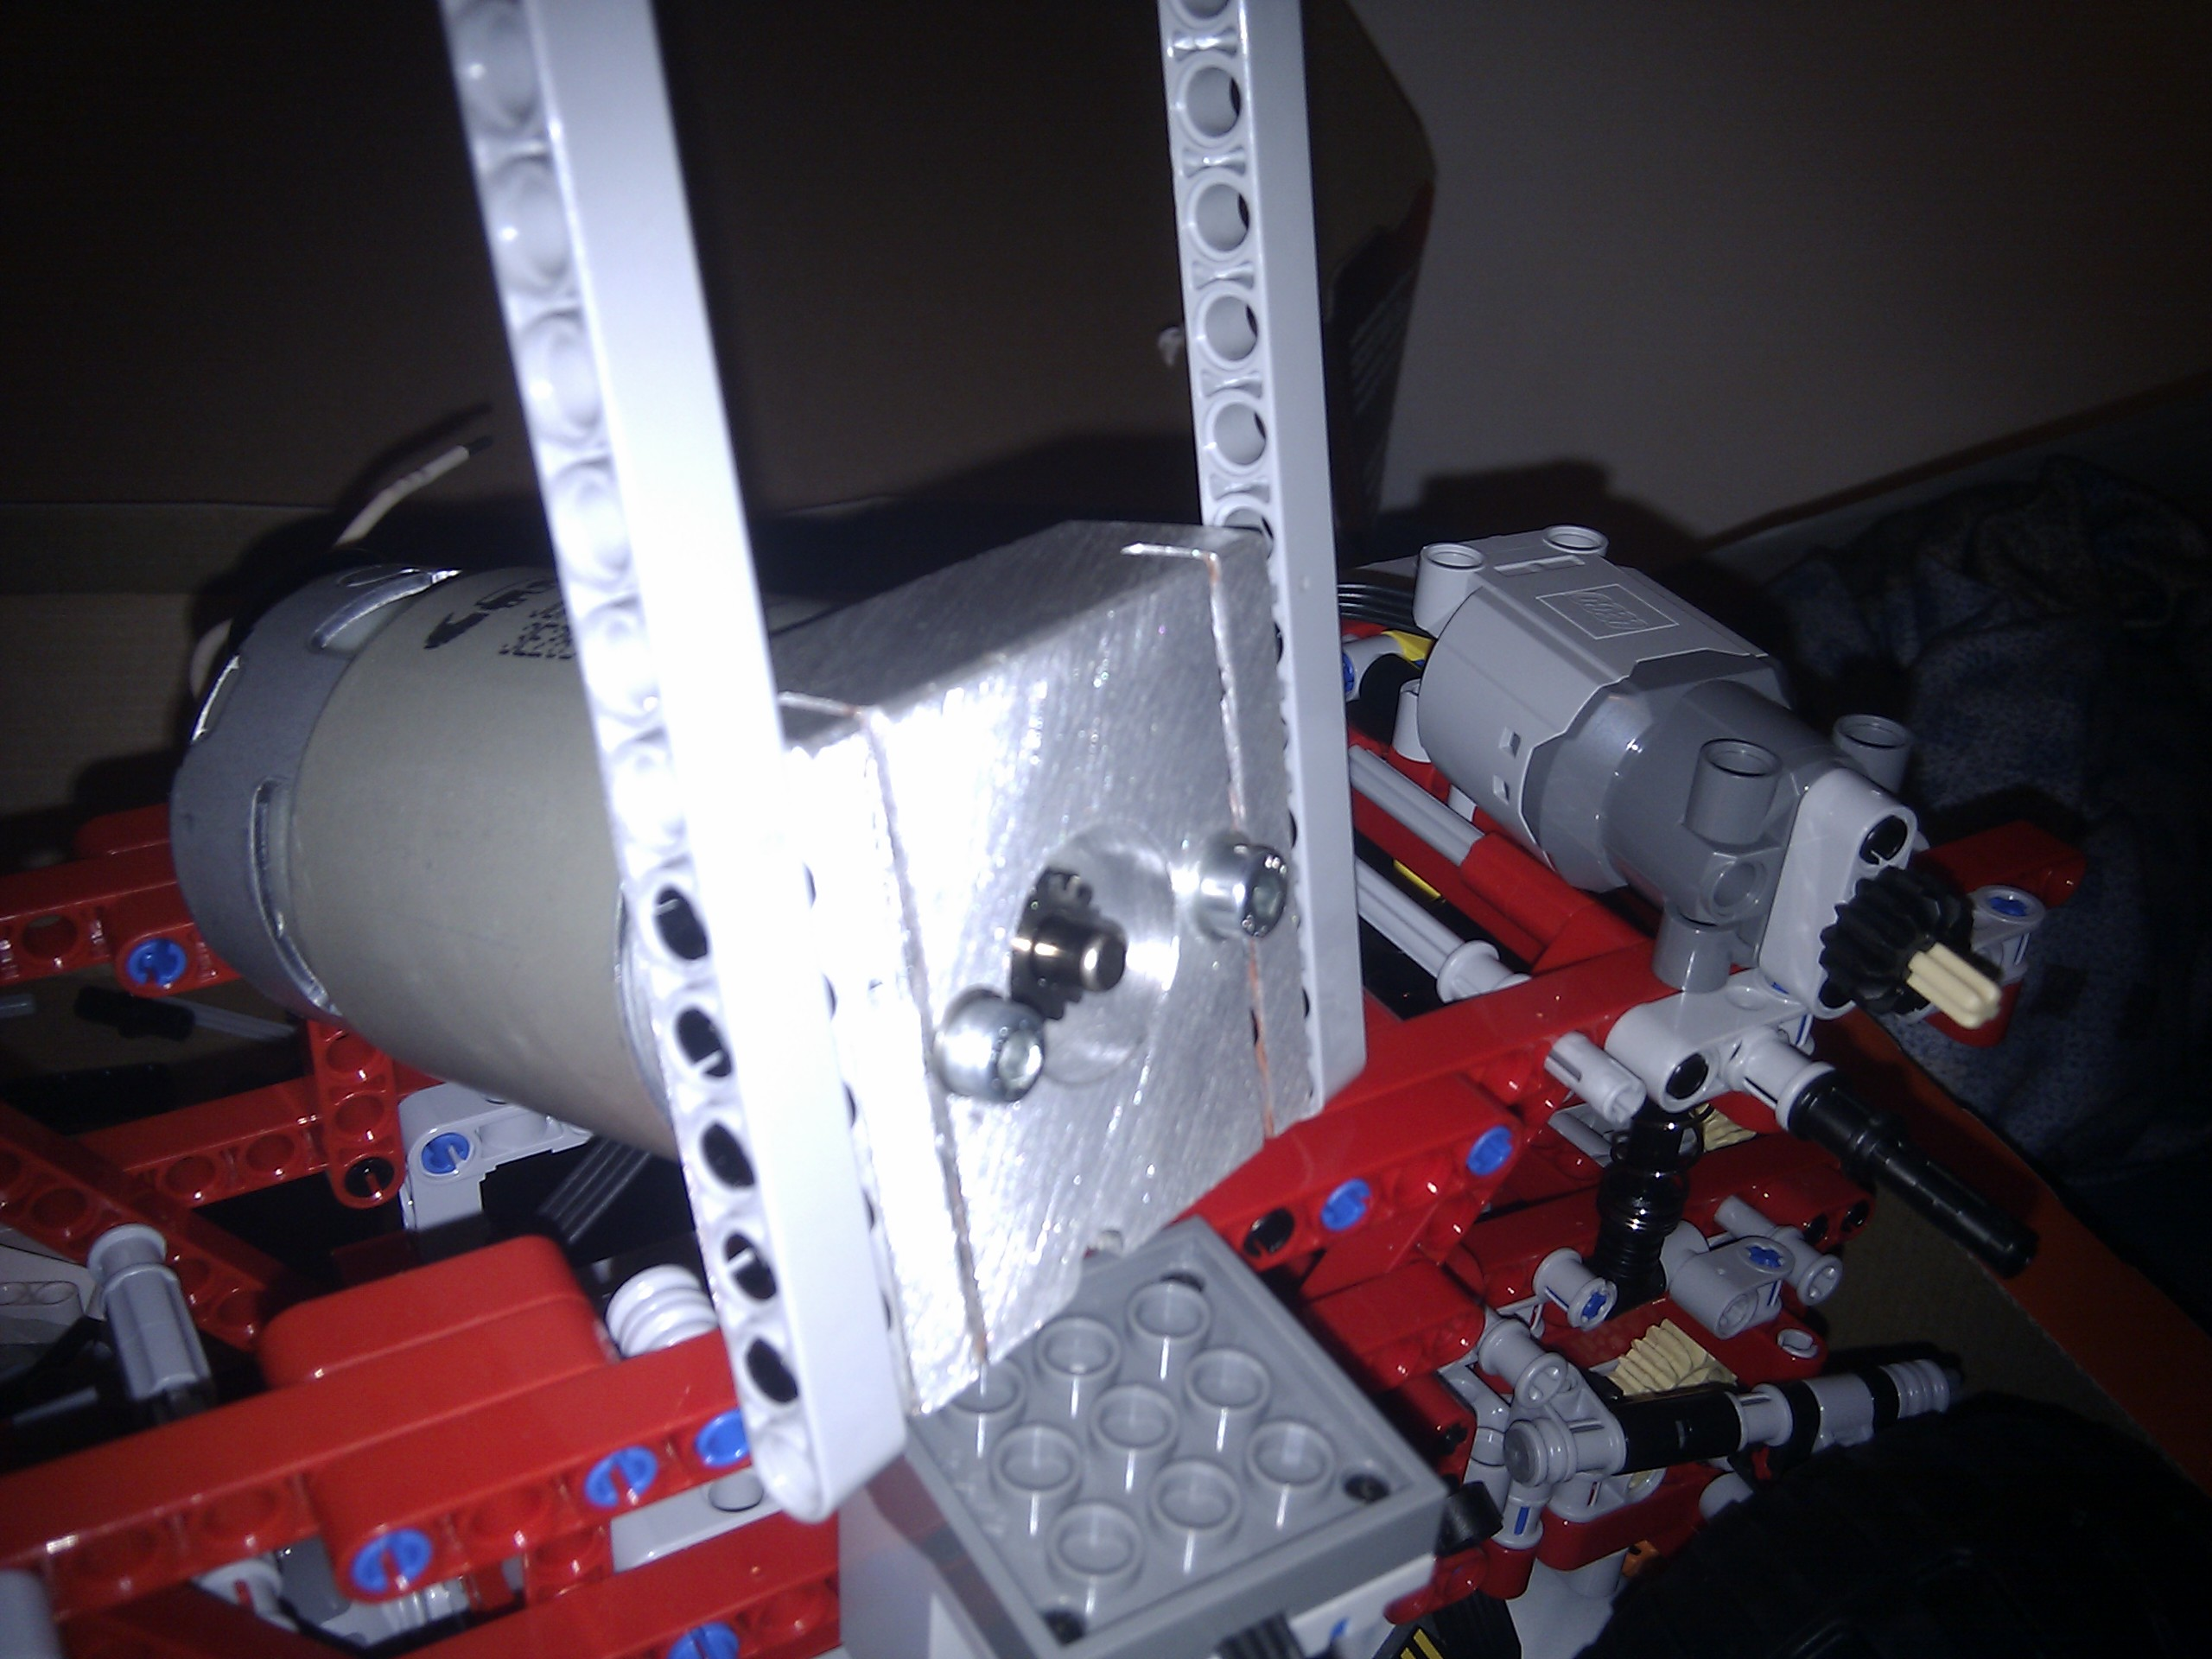
\includegraphics[width = \textwidth]{pics/raw/legomotor.jpg}
  \end{center}
\end{frame}

\section{RC Car}
\subsection{Original car}
\begin{frame}
  \begin{center}
  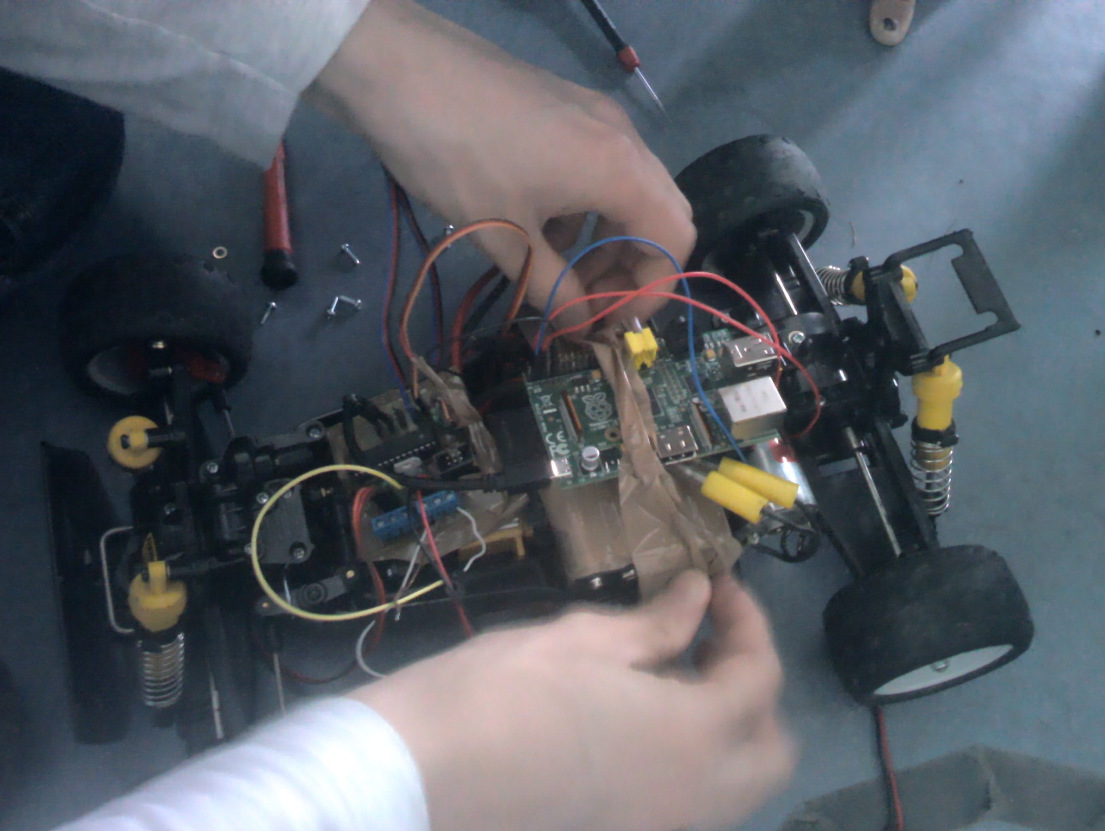
\includegraphics[width = \textwidth]{pics/raw/original.png}
  \end{center}
\end{frame}

\subsection{Wood board}
\begin{frame}
  \begin{center}
  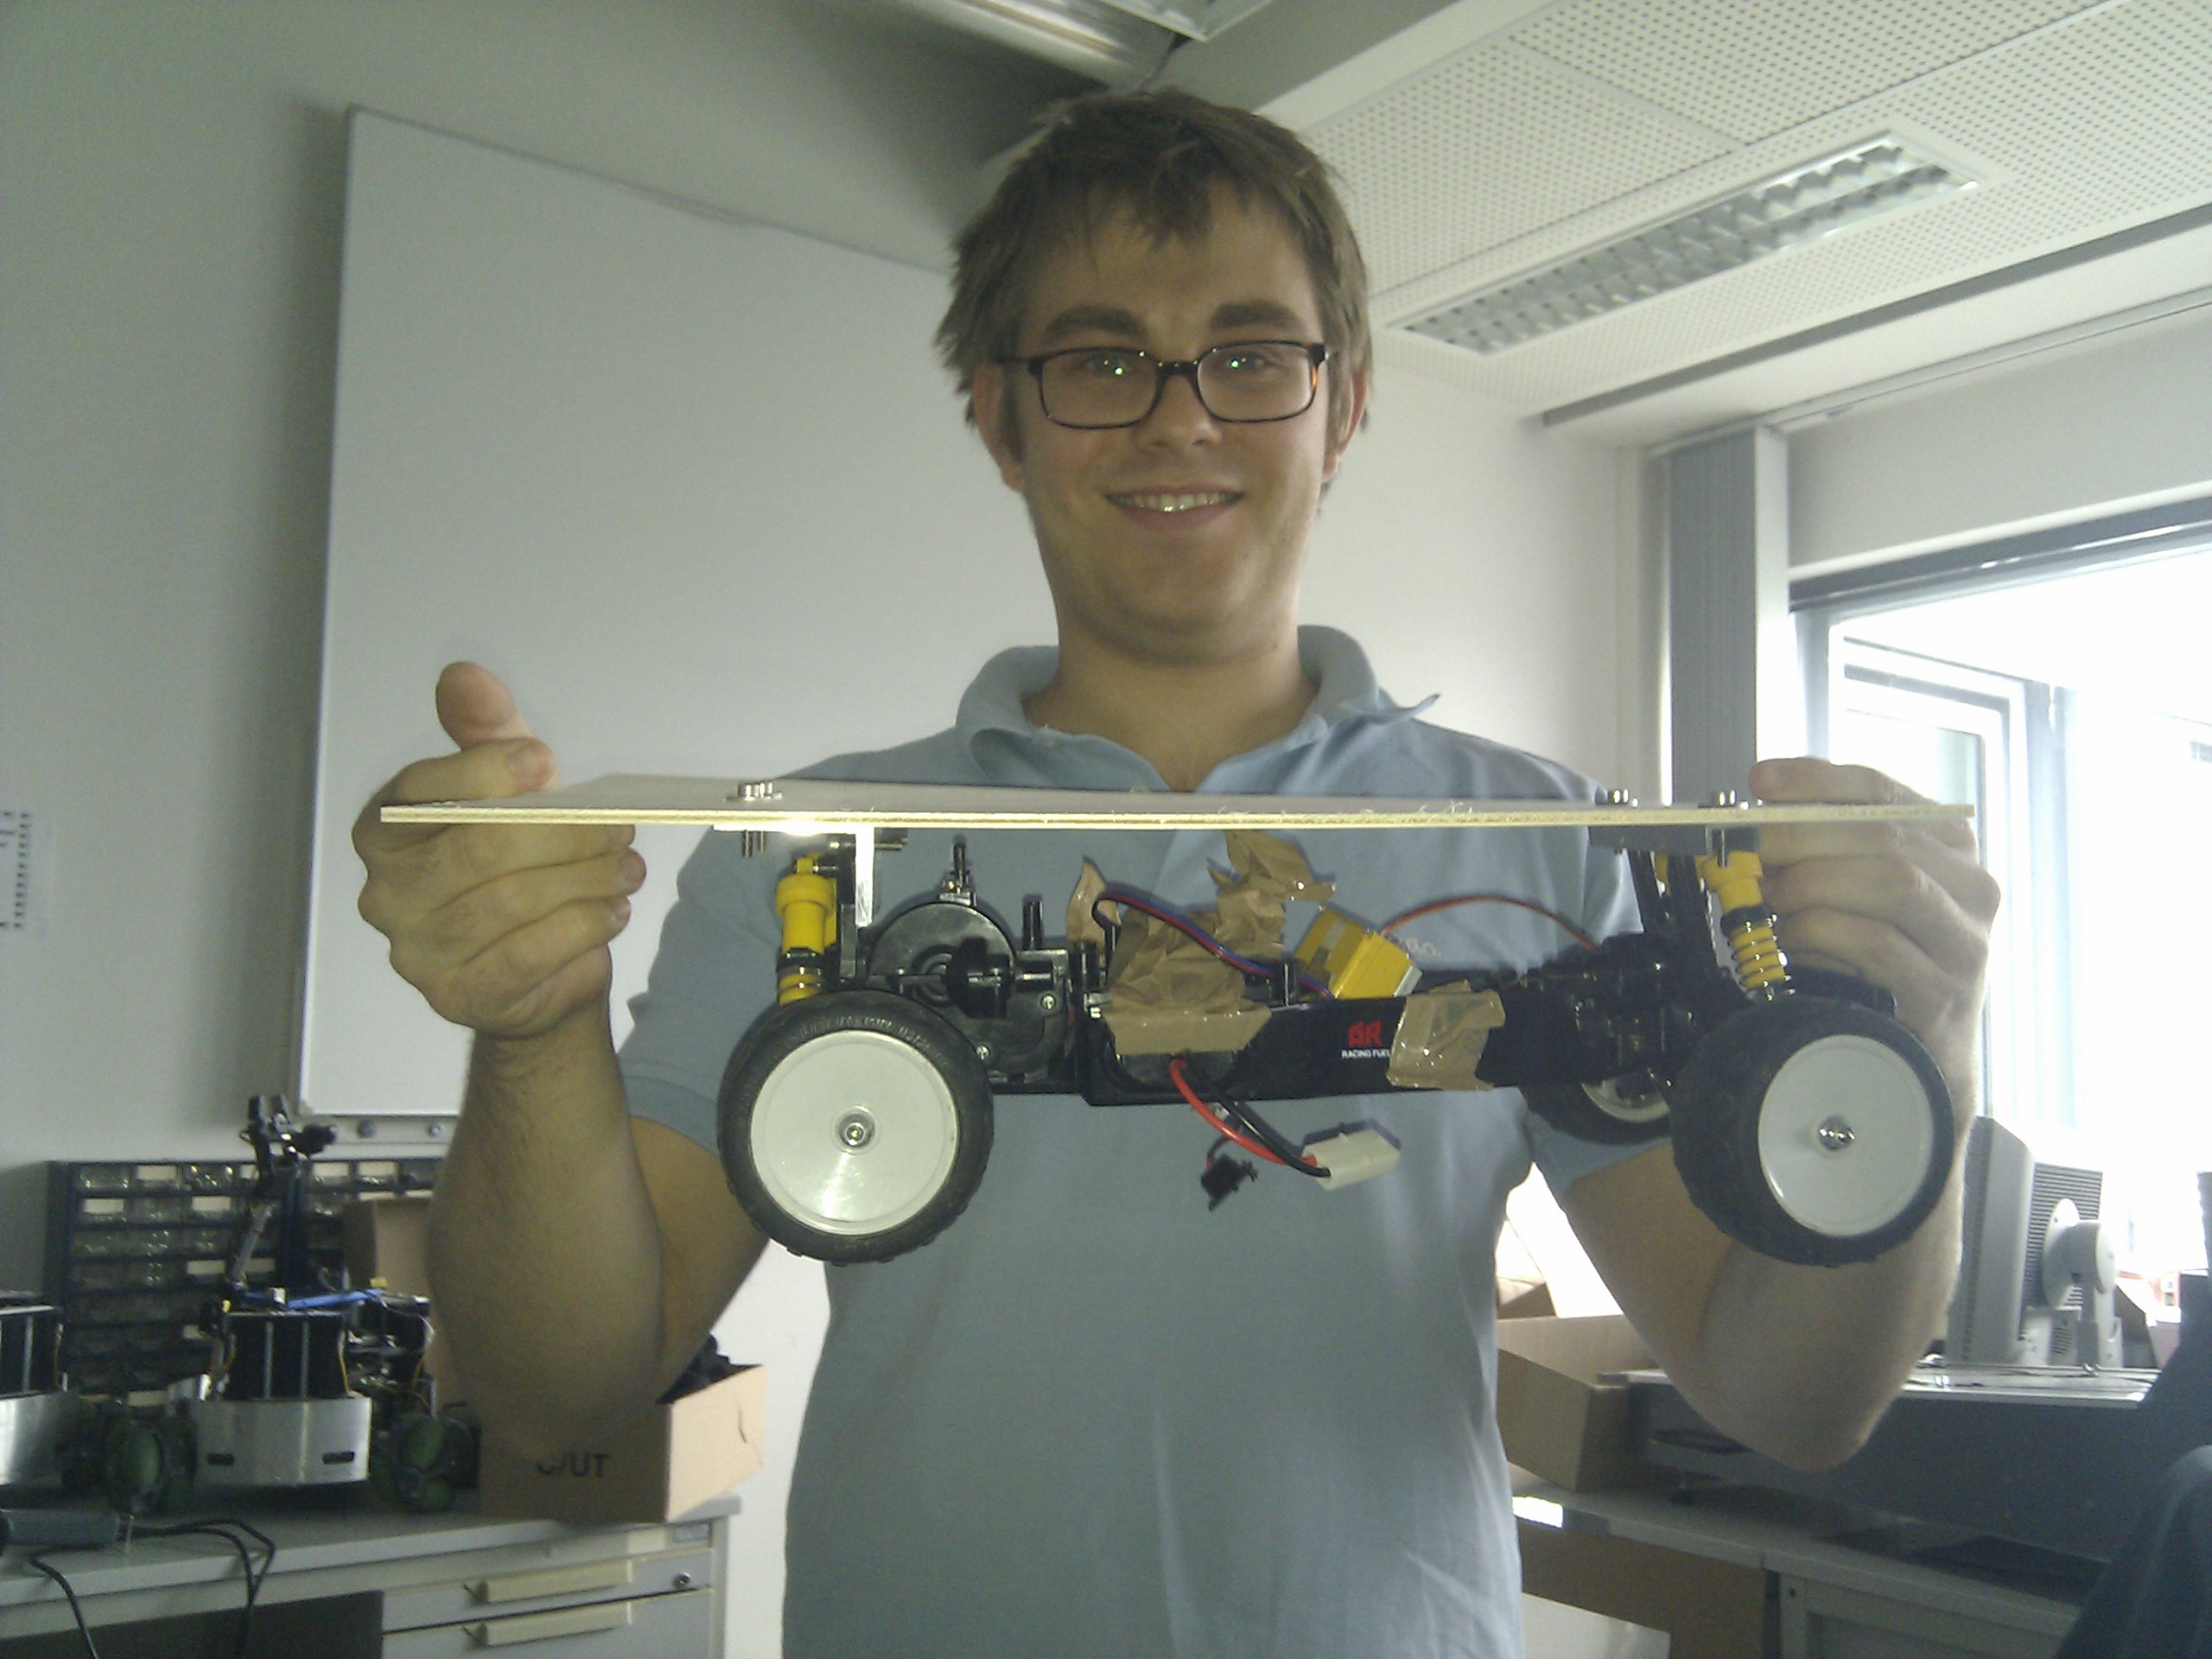
\includegraphics[width = \textwidth]{pics/raw/brett.jpg}
  \end{center}
\end{frame}
\subsection{Metal enhancement}

\begin{frame}
  \begin{center}
  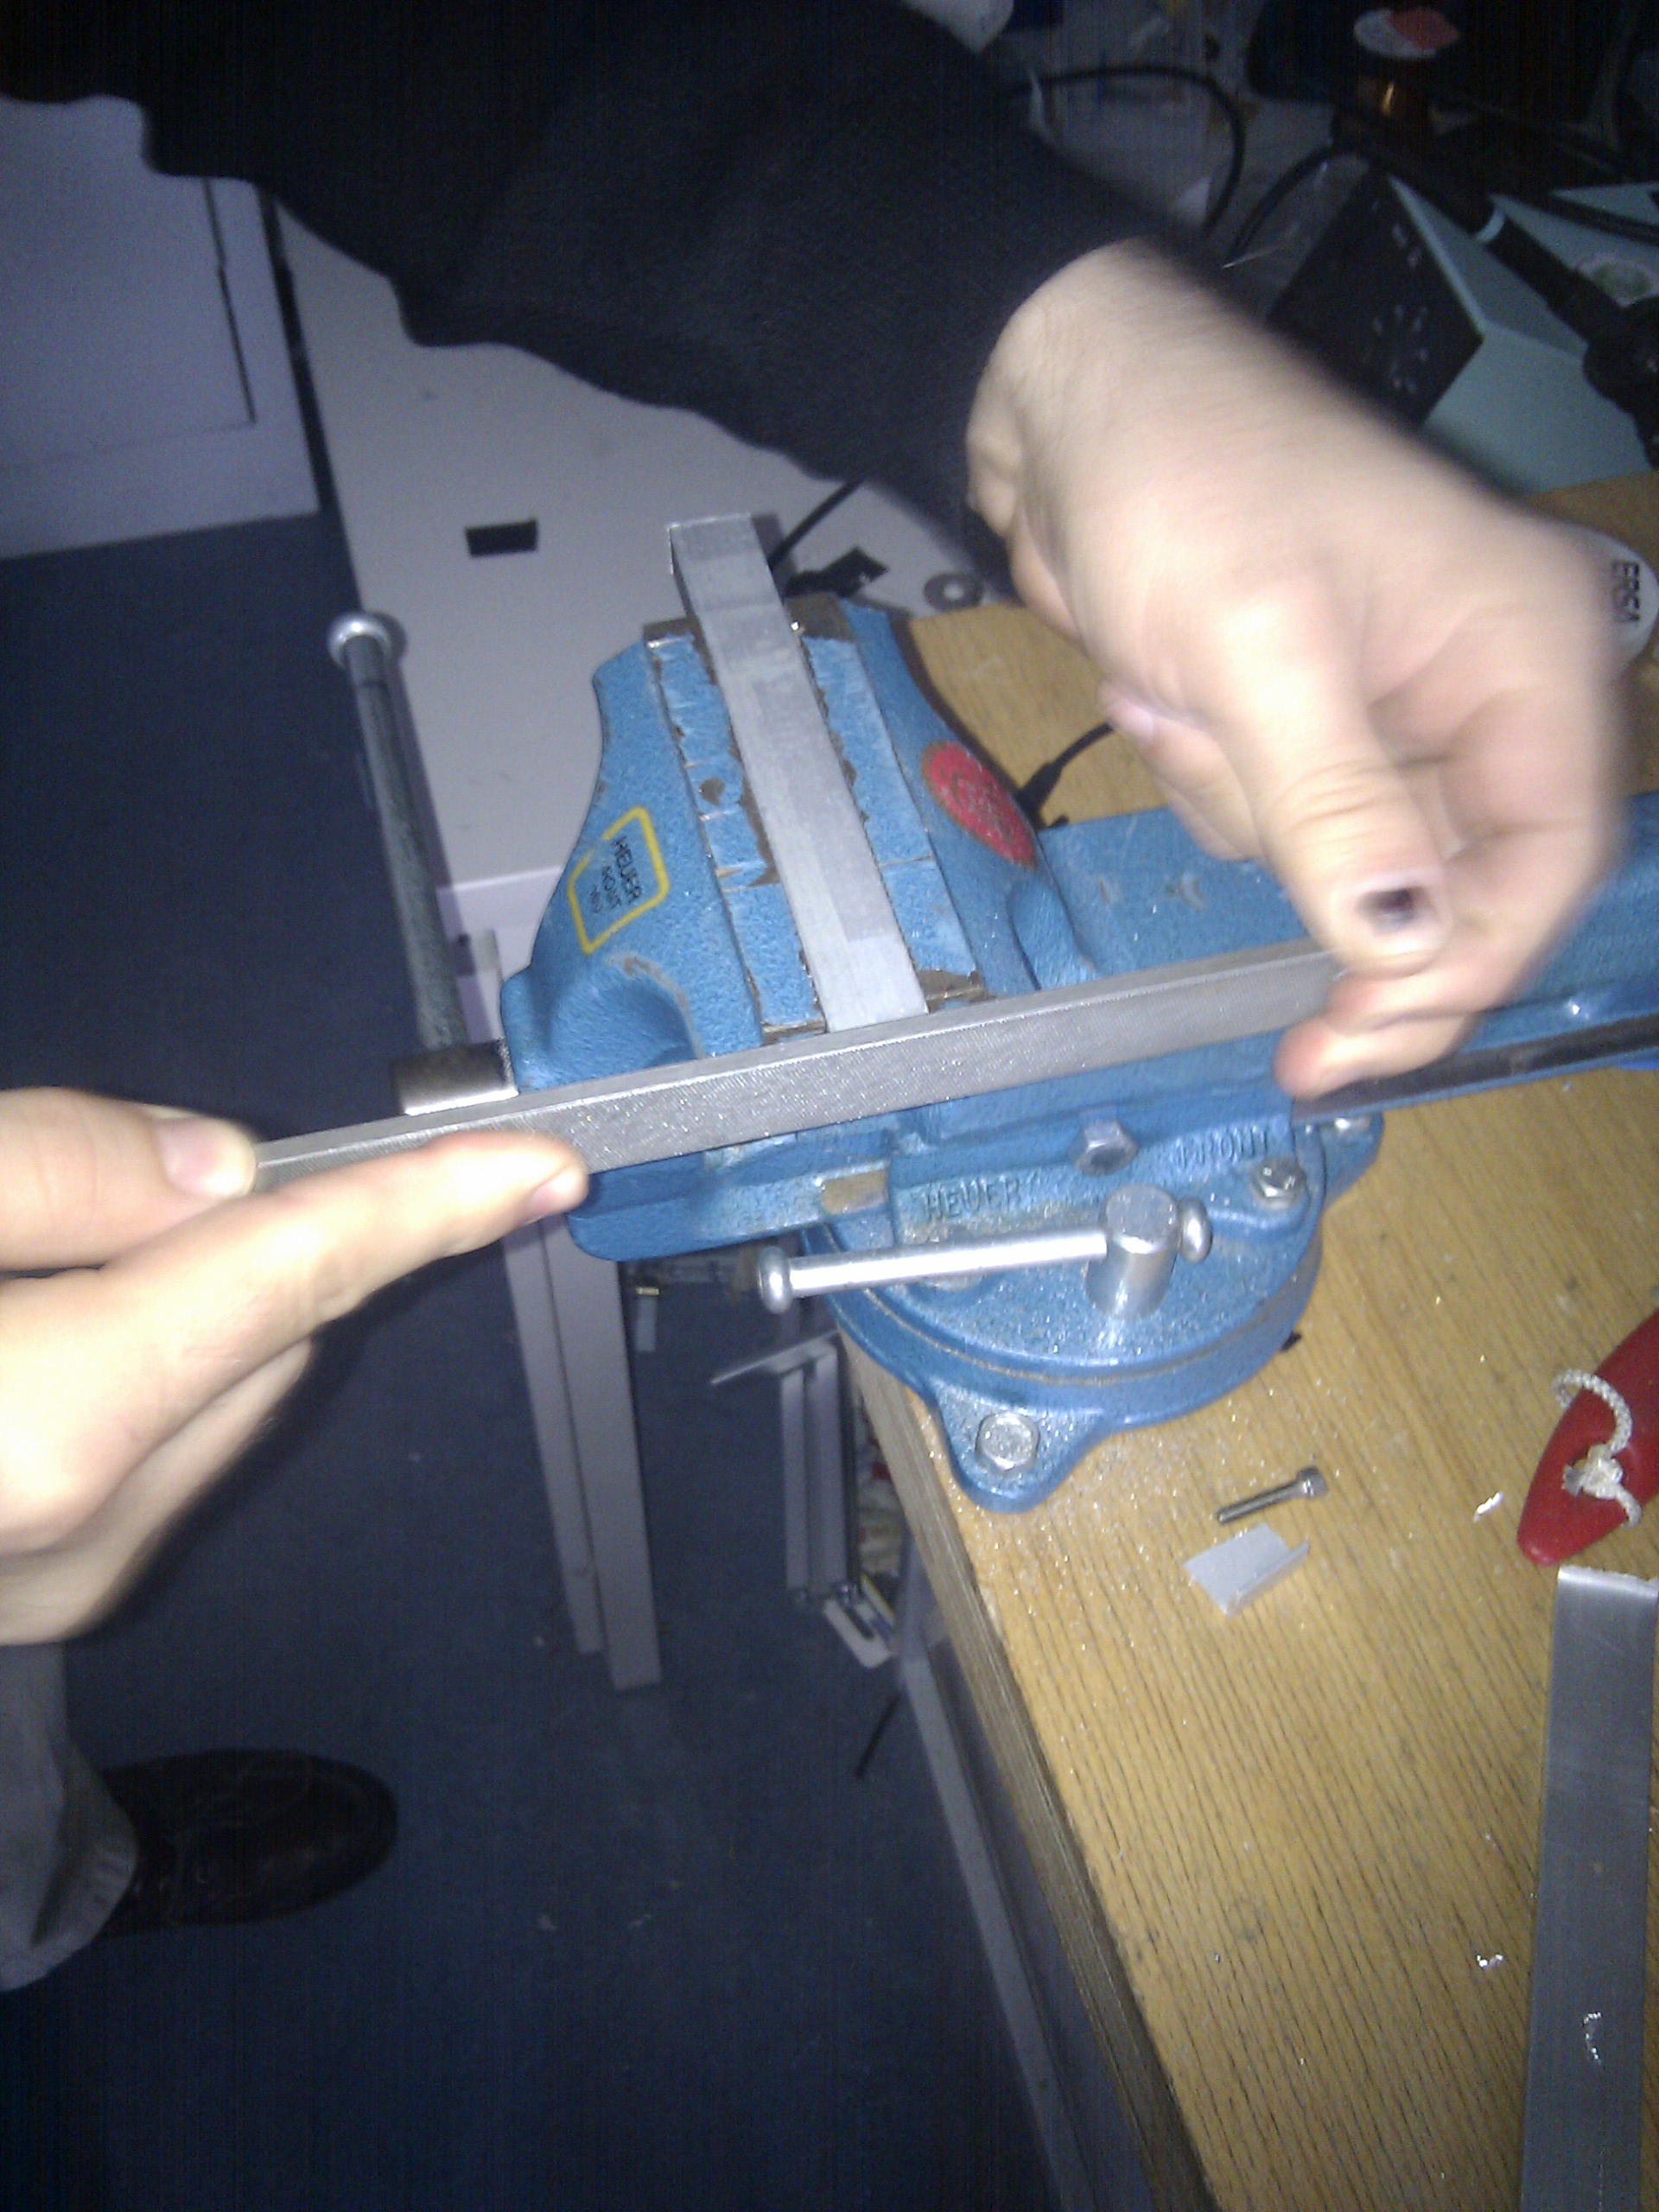
\includegraphics[width = \textwidth]{pics/raw/feilen.jpg}
  \end{center}
\end{frame}

\begin{frame}
  \begin{center}
  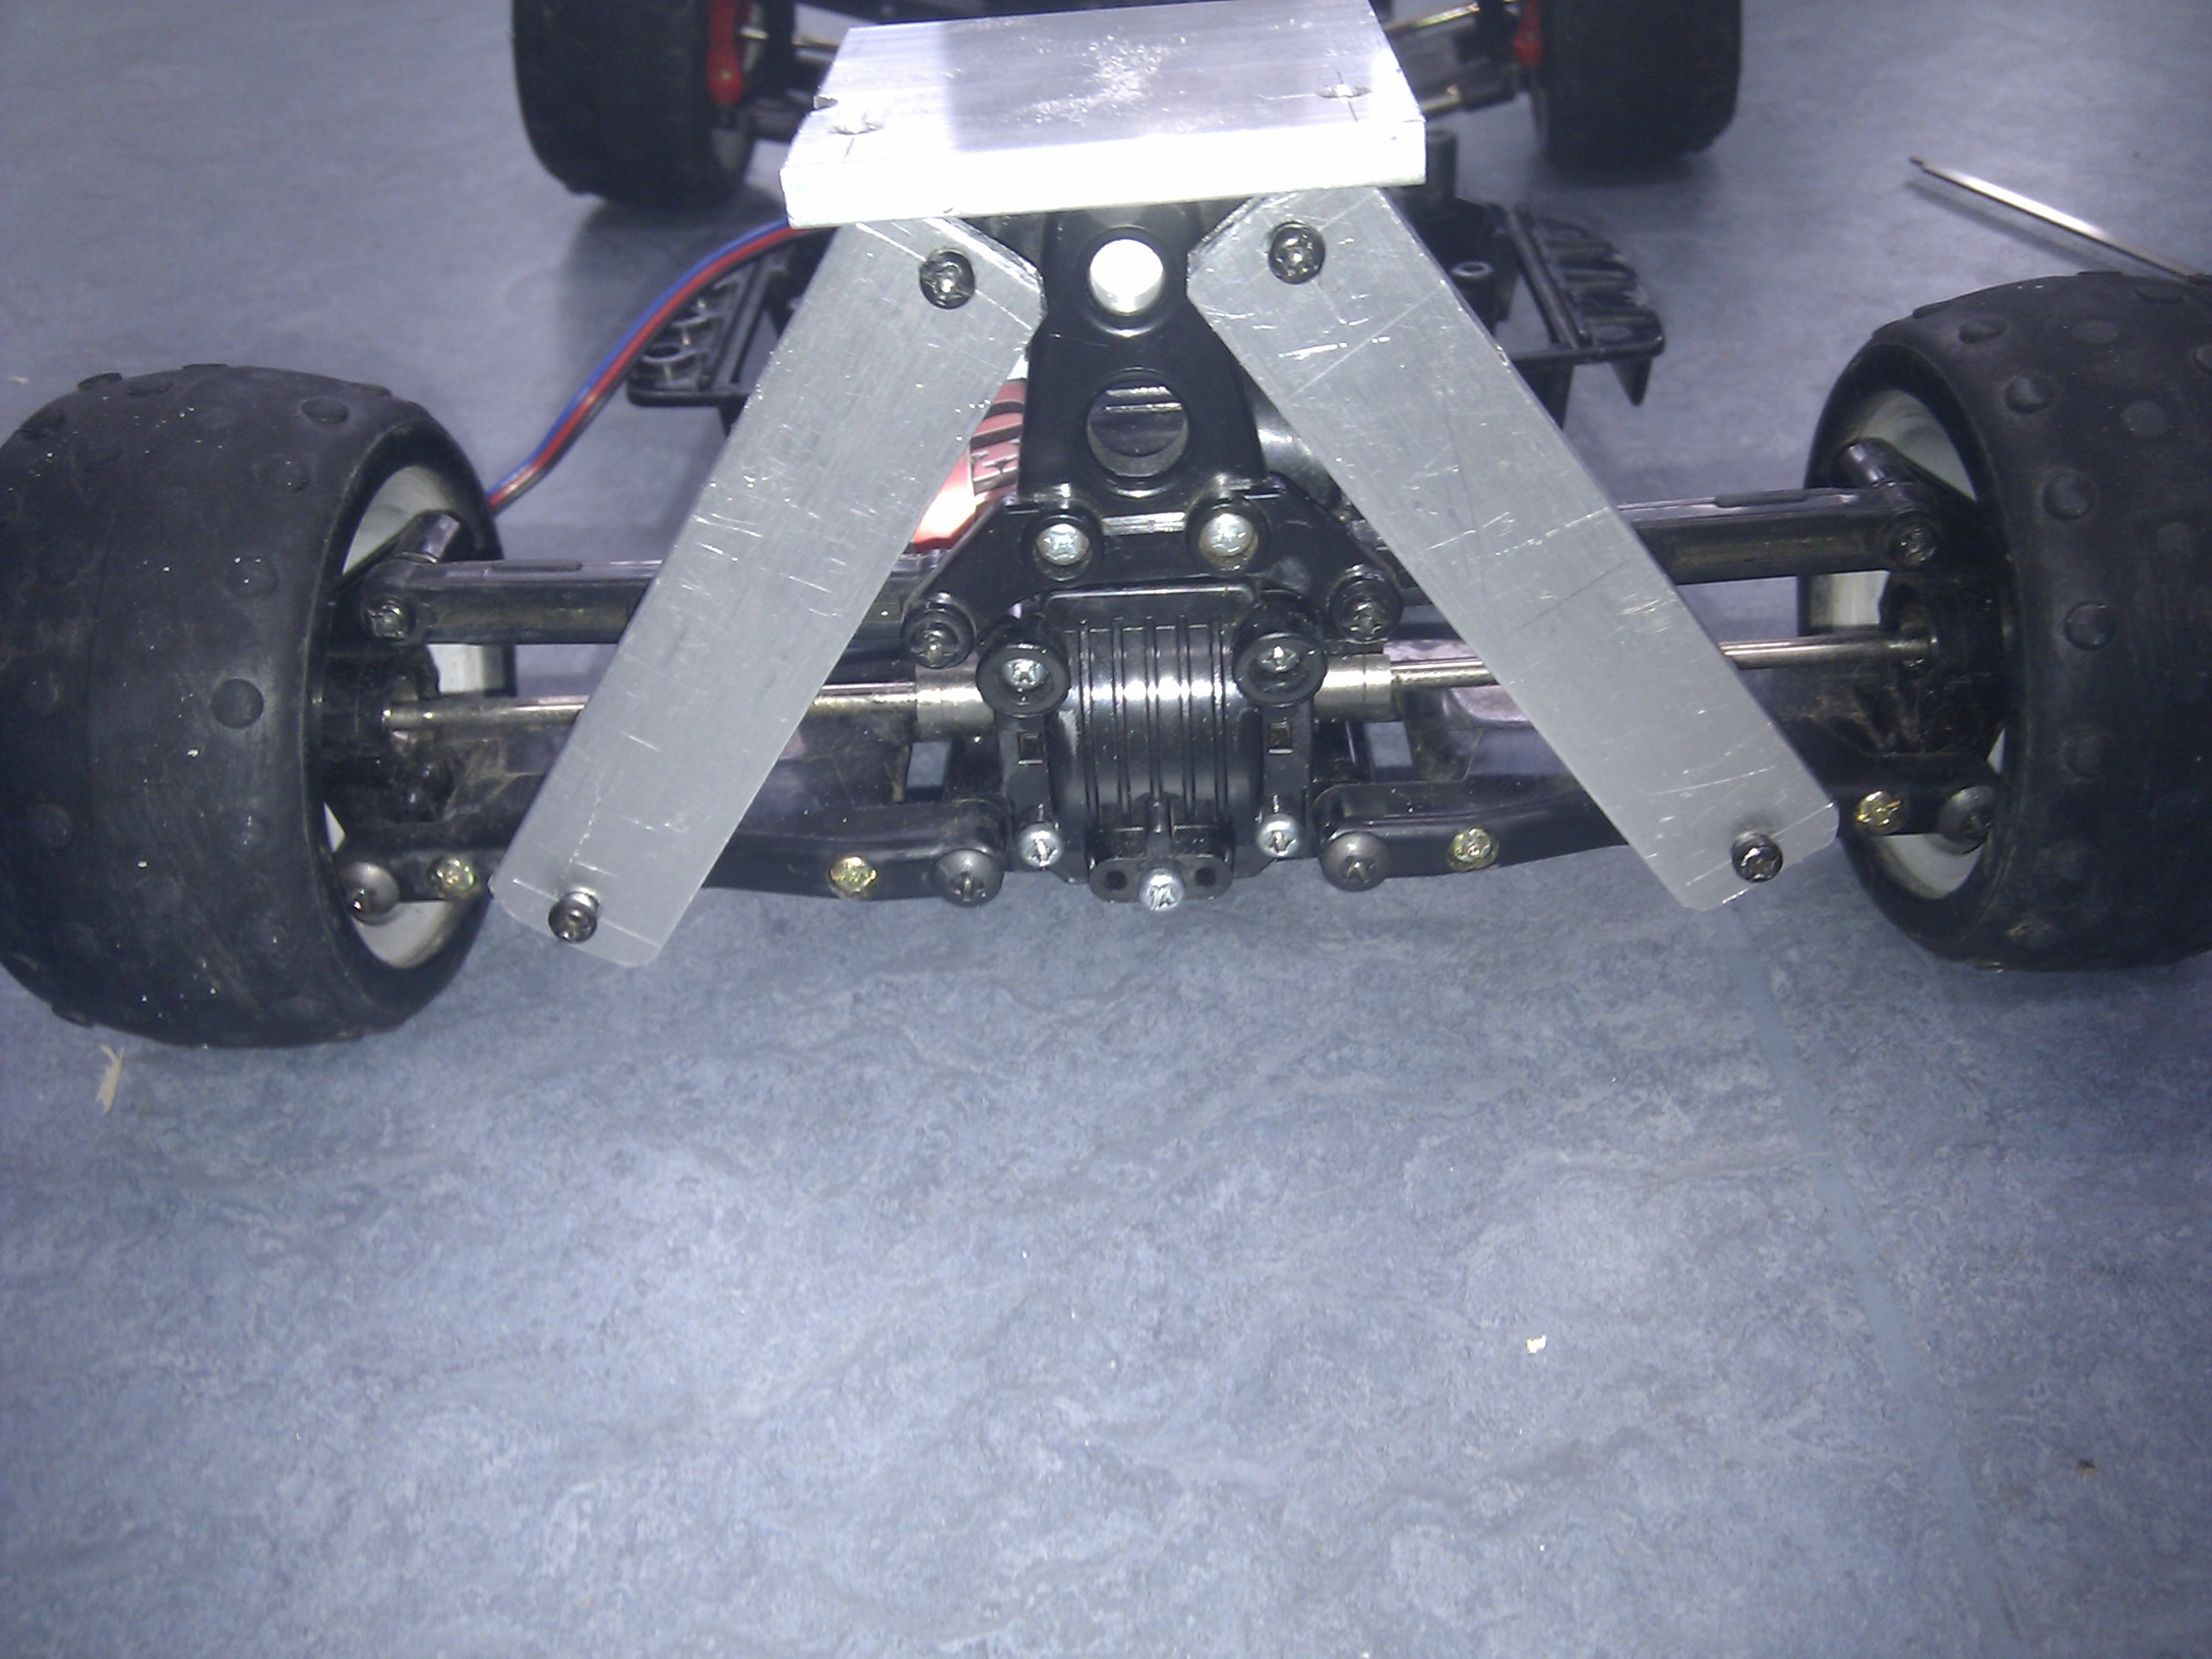
\includegraphics[width = \textwidth]{pics/raw/car_back_ueberarbeitet.jpg}
  \end{center}
\end{frame}

\begin{frame}
  \begin{center}
  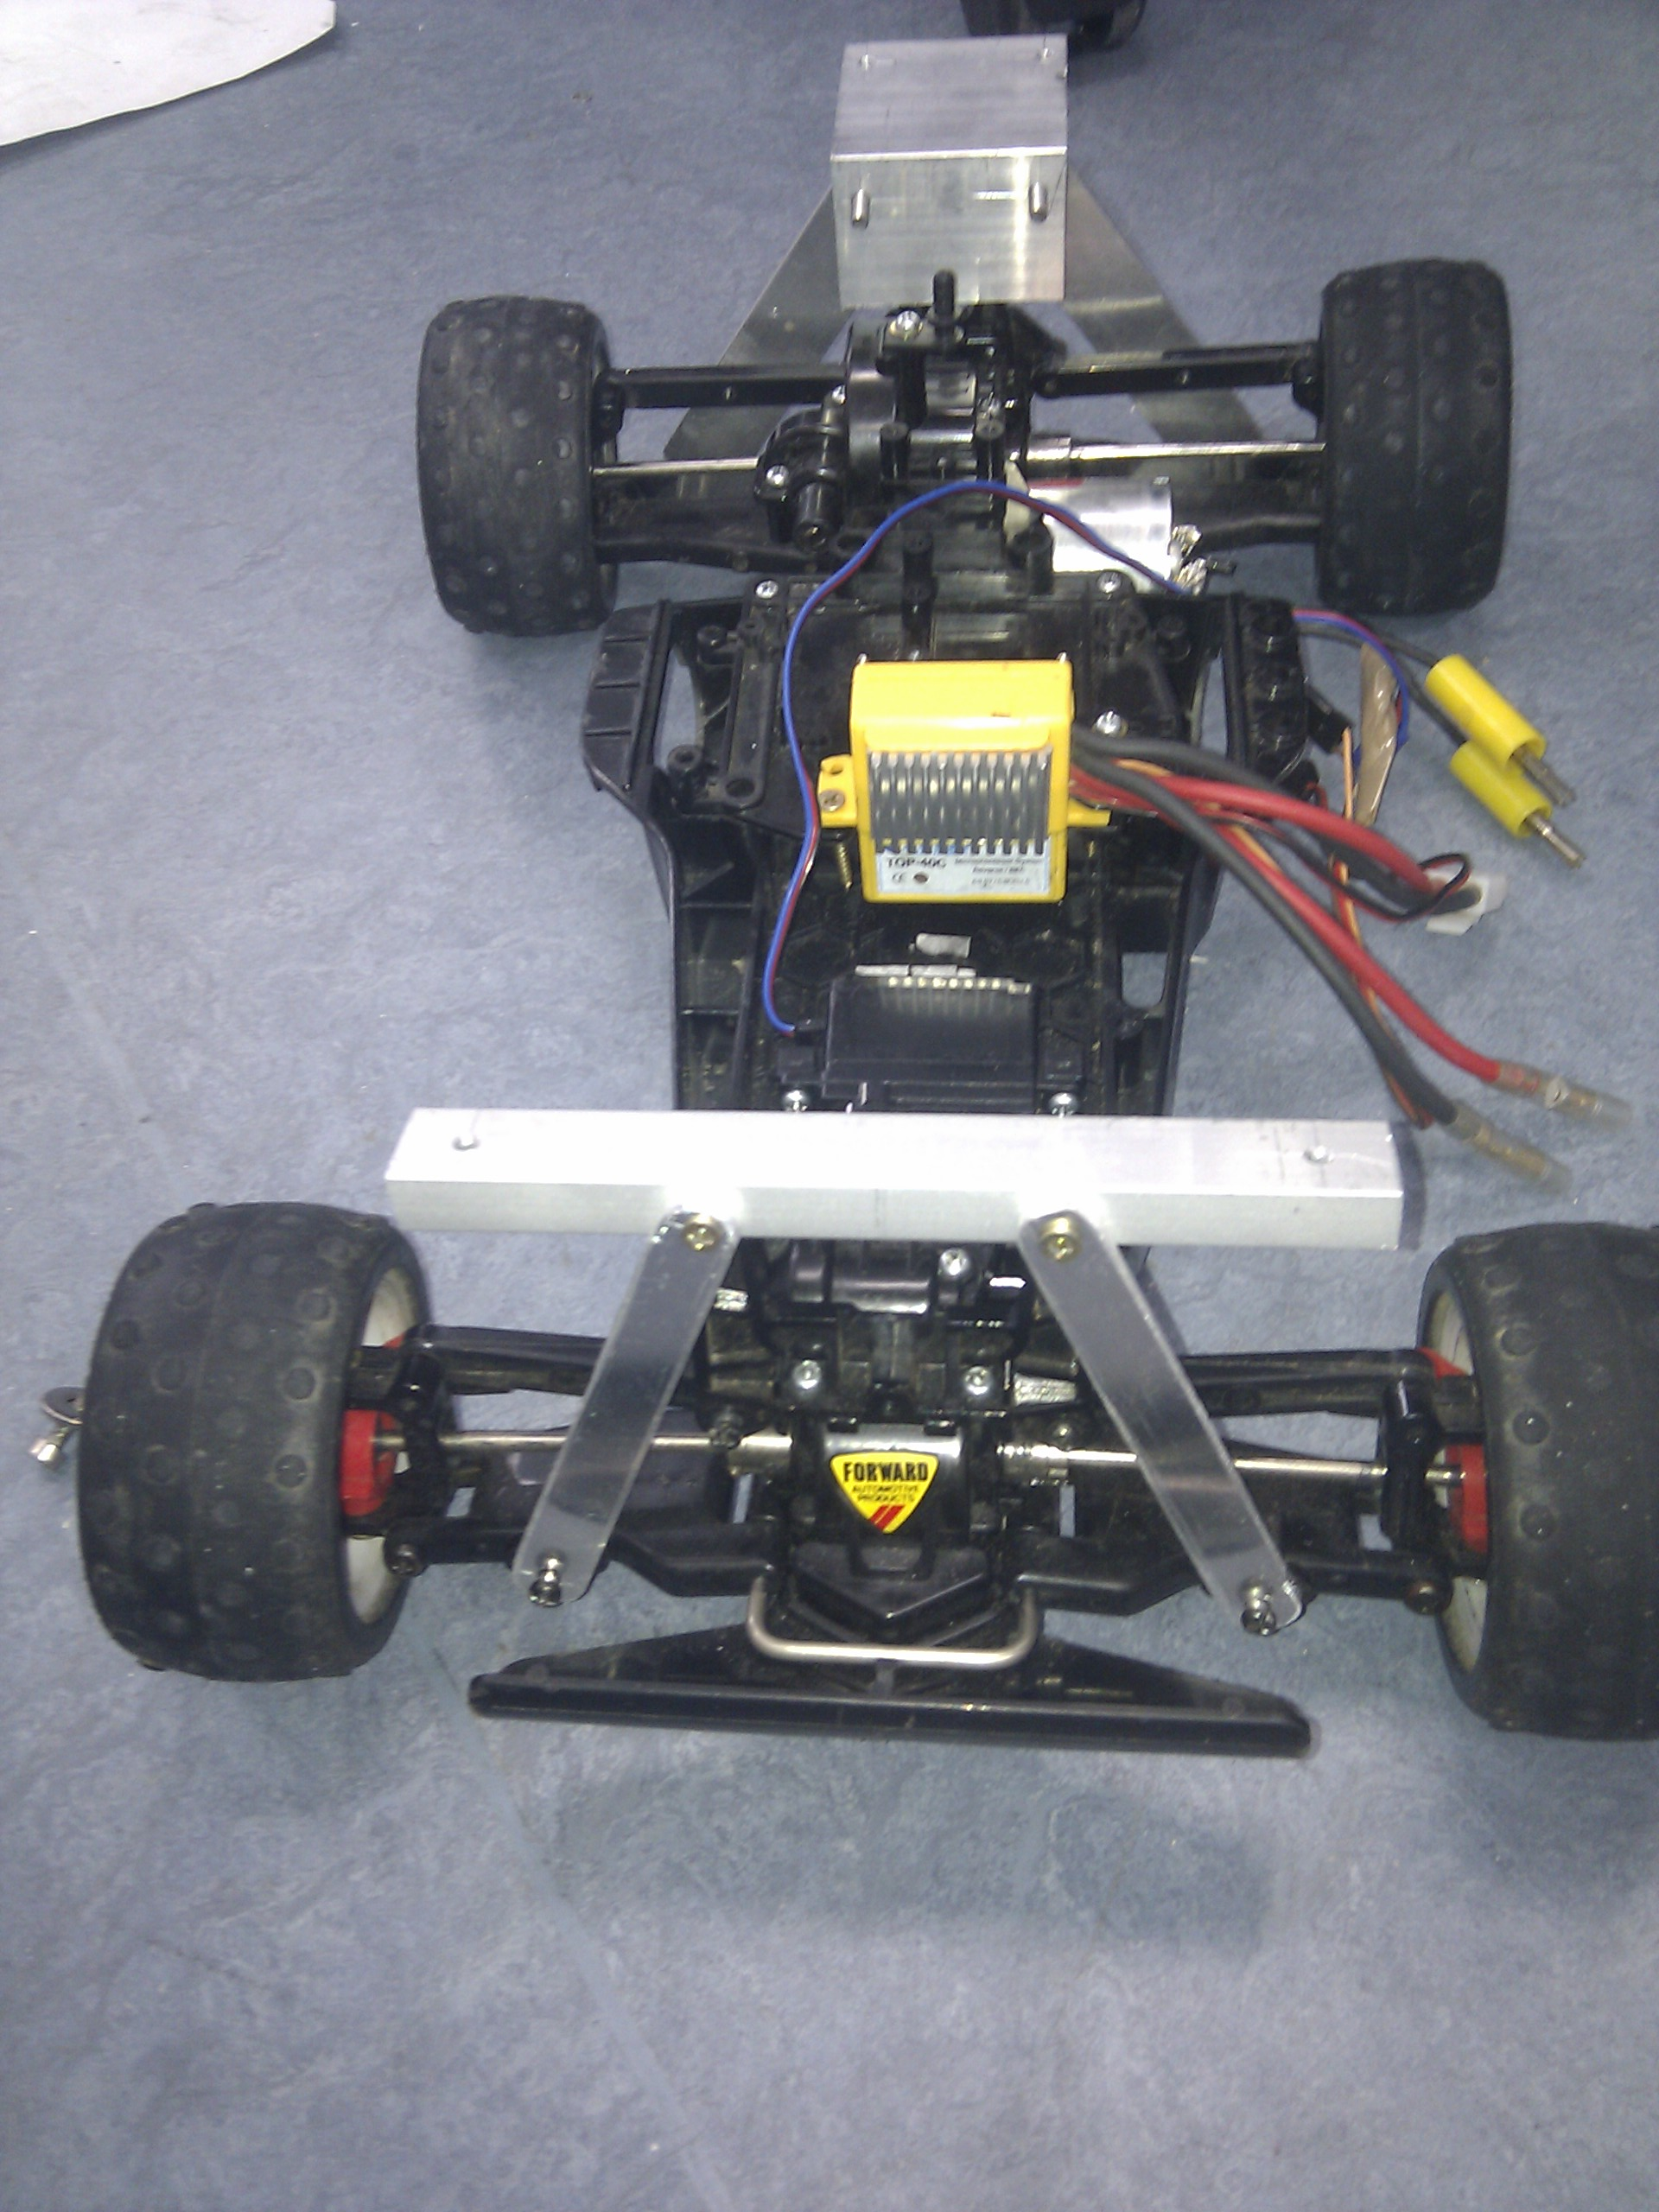
\includegraphics[width = 0.6\textwidth]{pics/raw/car_enhanced.jpg}
  \end{center}
\end{frame}

\section{Electronics}
\subsection{Custom built PCB}
\begin{frame}
  \begin{center}
  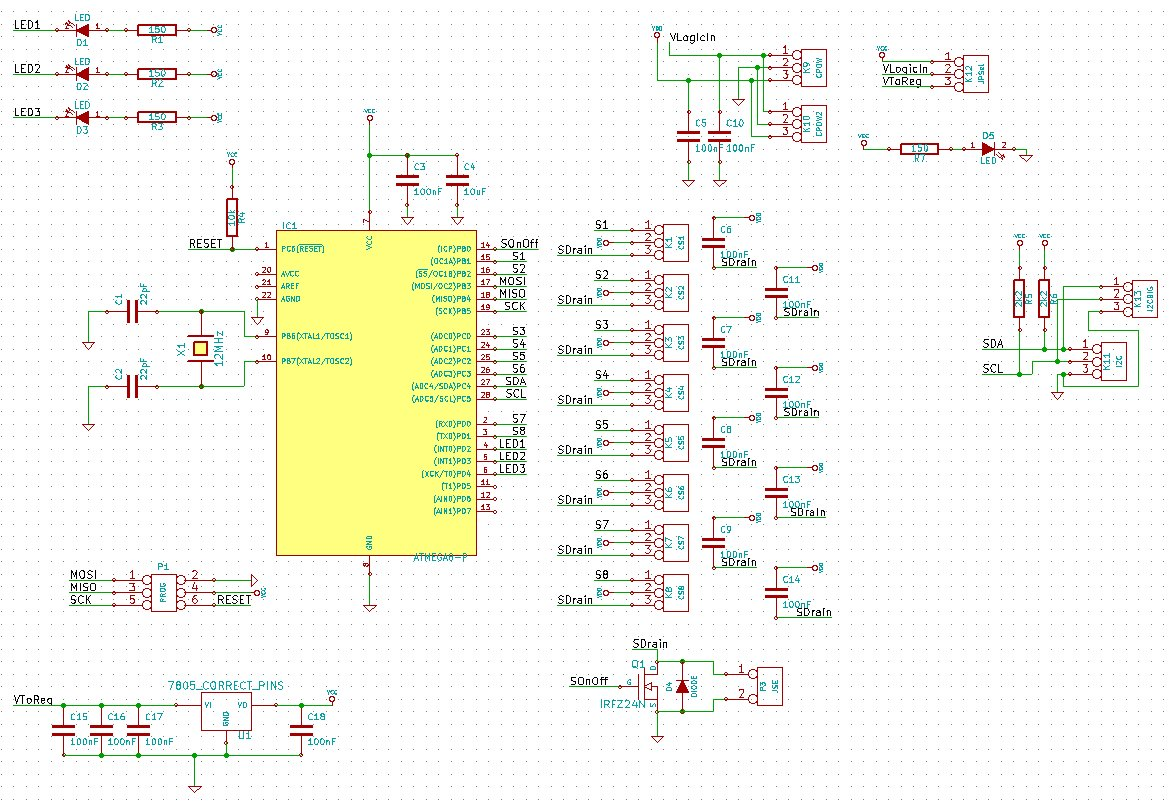
\includegraphics[width = \textwidth]{pics/raw/sensor_scem.png}
  \end{center}
\end{frame}

\begin{frame}
  \begin{center}
  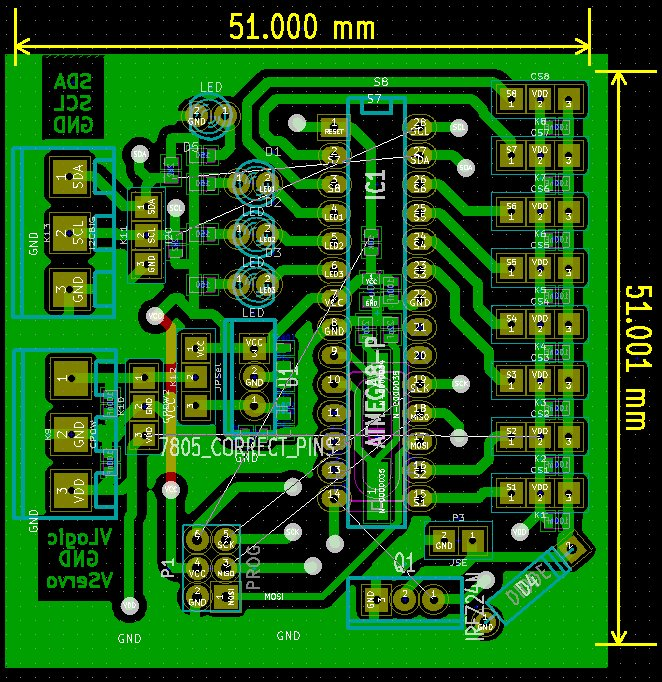
\includegraphics[width = 0.7\textwidth]{pics/raw/serrvo_brd.png}
  \end{center}
\end{frame}

\begin{frame}
  \begin{center}
  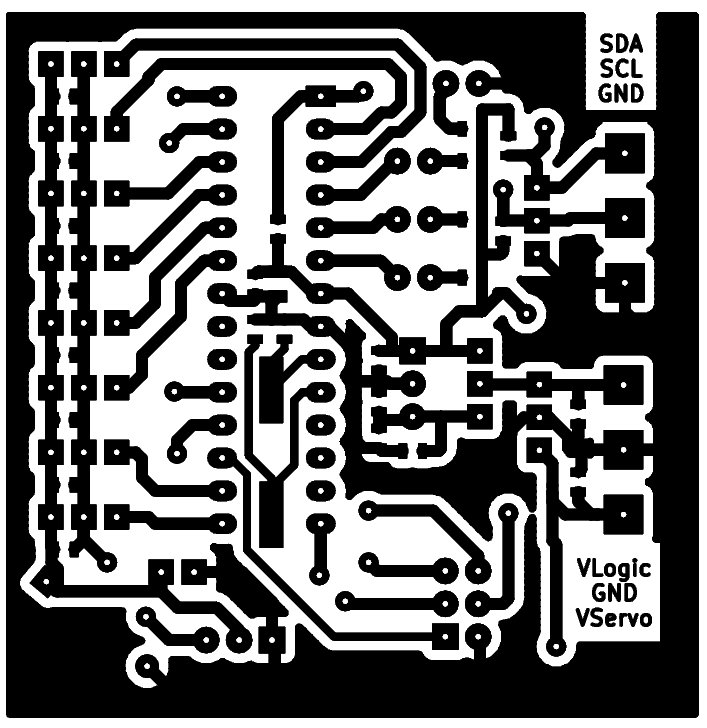
\includegraphics[width = 0.7\textwidth]{pics/raw/servoboard_plot.png}
  \end{center}
\end{frame}

\begin{frame}
  \begin{center}
  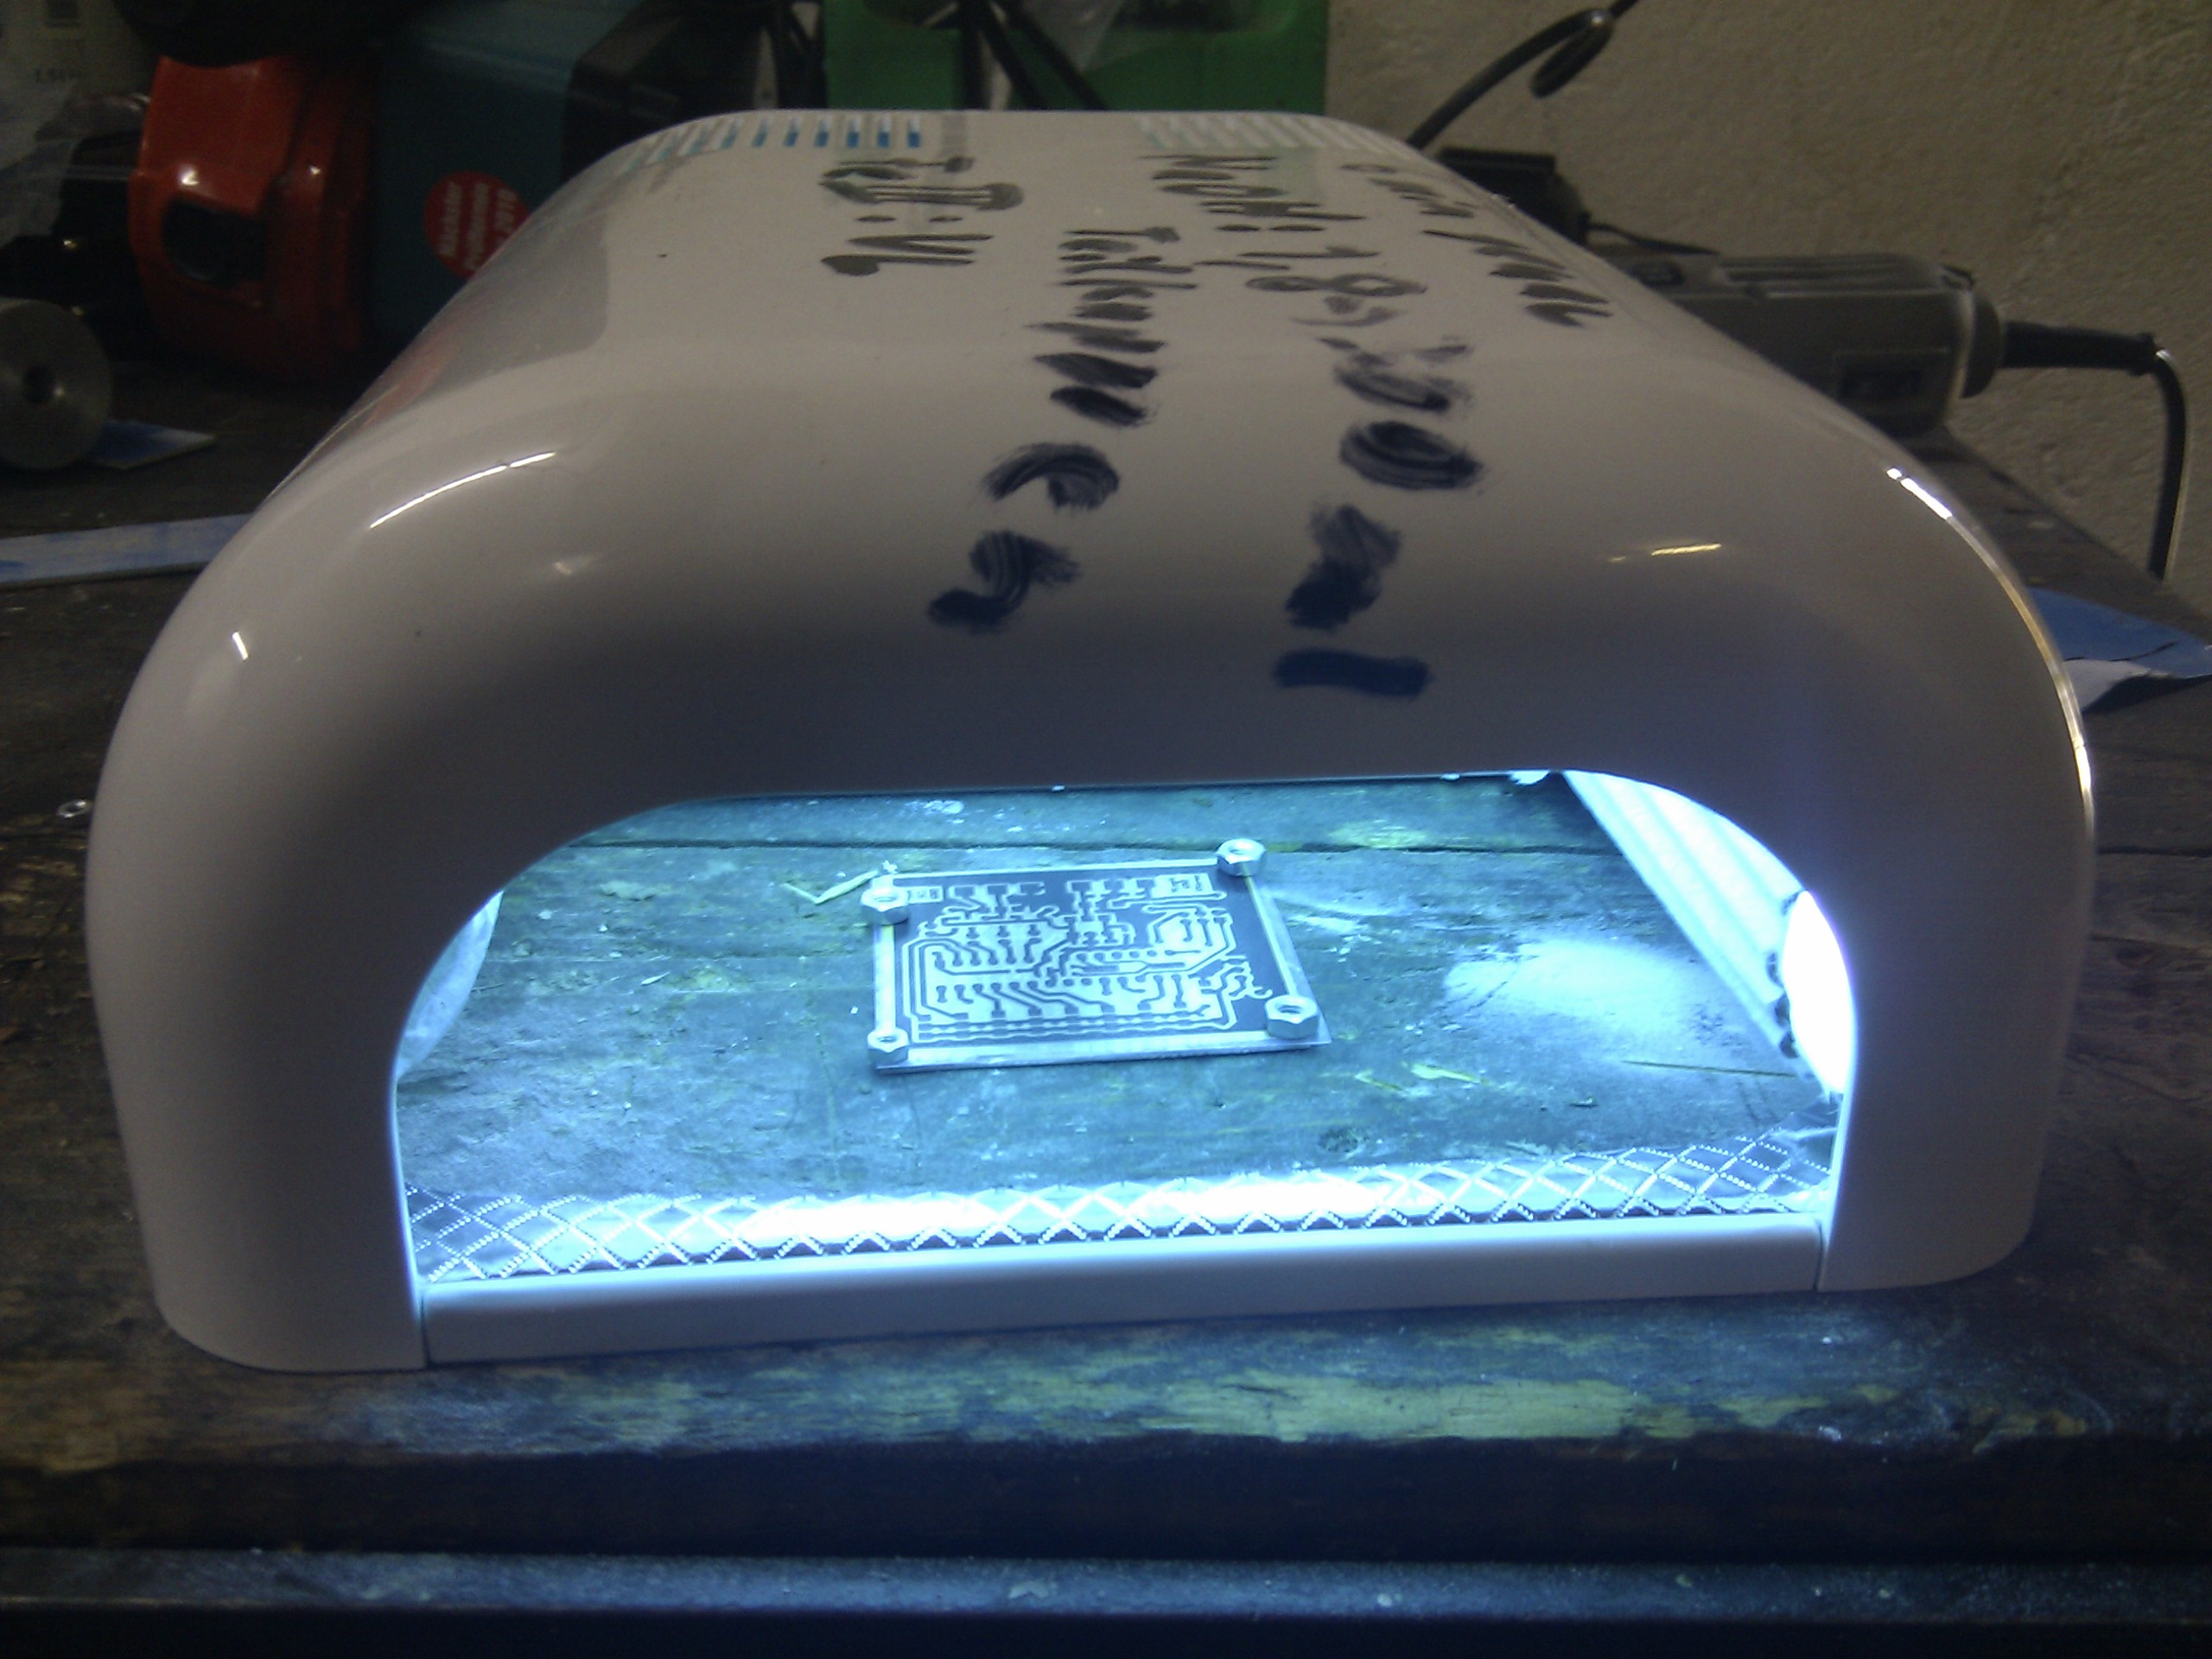
\includegraphics[width = \textwidth]{pics/raw/servoboard_light.jpg}
  \end{center}
\end{frame}

\begin{frame}
  \begin{center}
  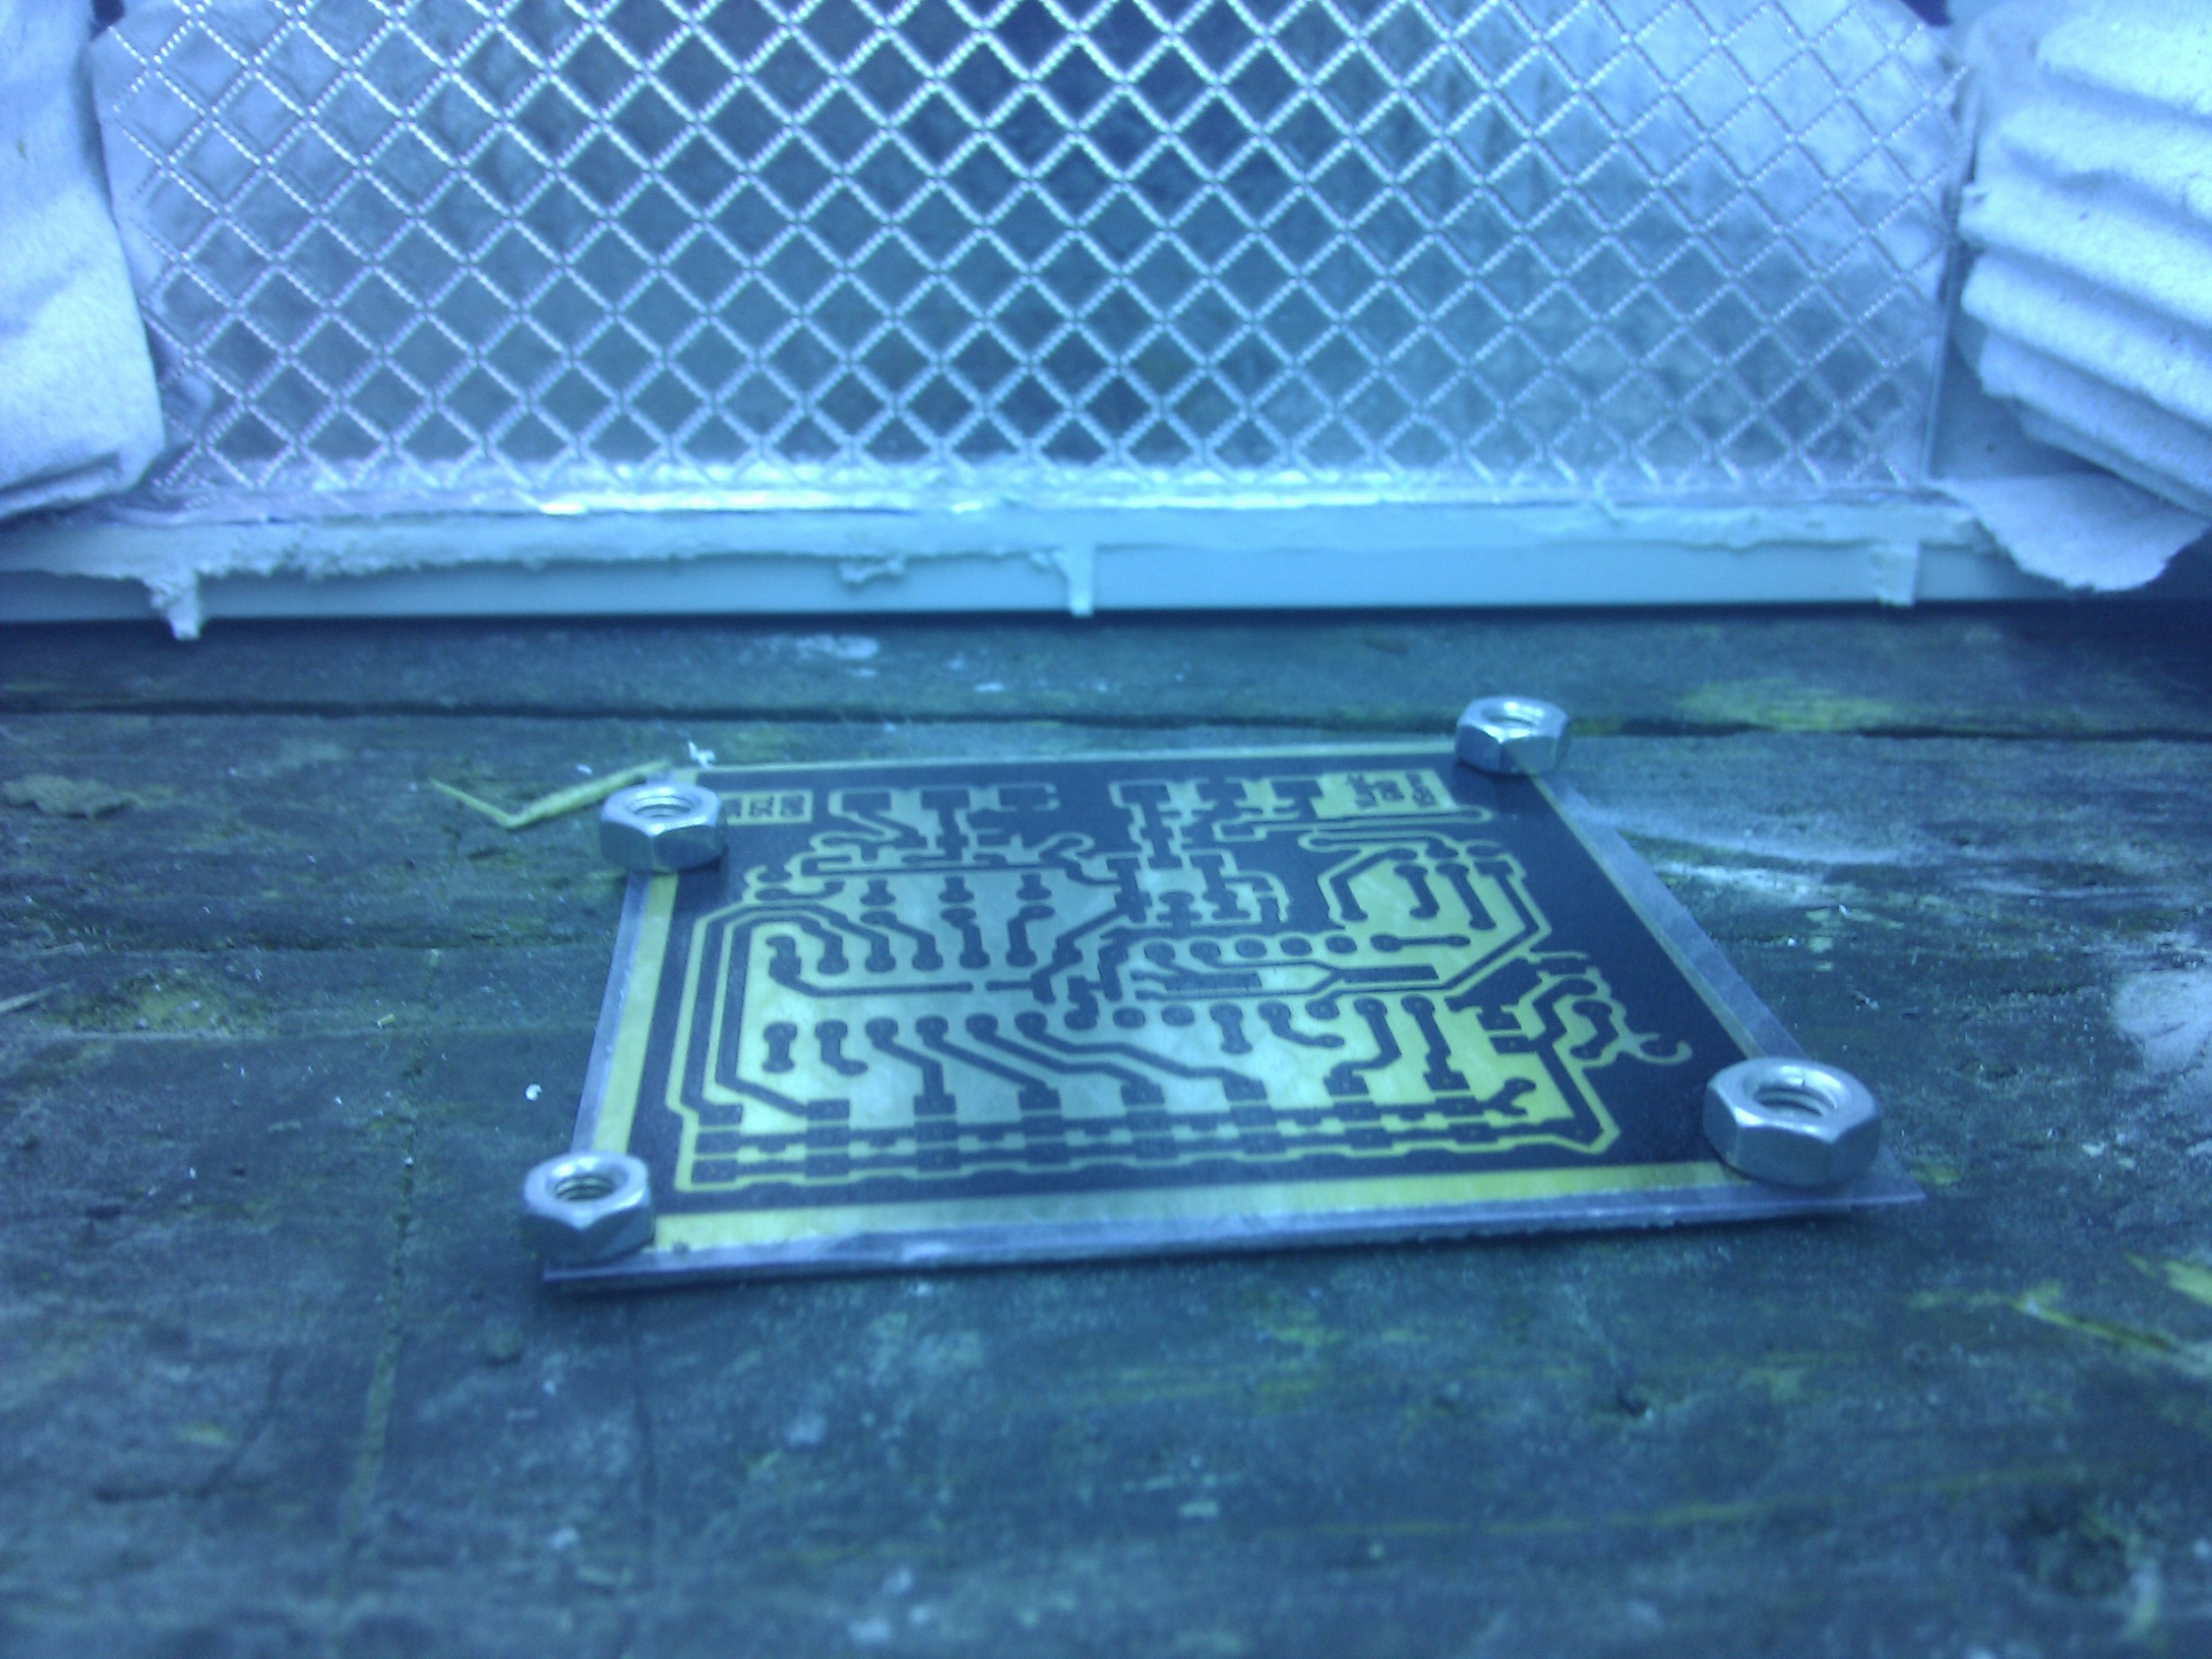
\includegraphics[width = \textwidth]{pics/raw/servoboard_ligt2.jpg}
  \end{center}
\end{frame}

\begin{frame}
  \begin{center}
  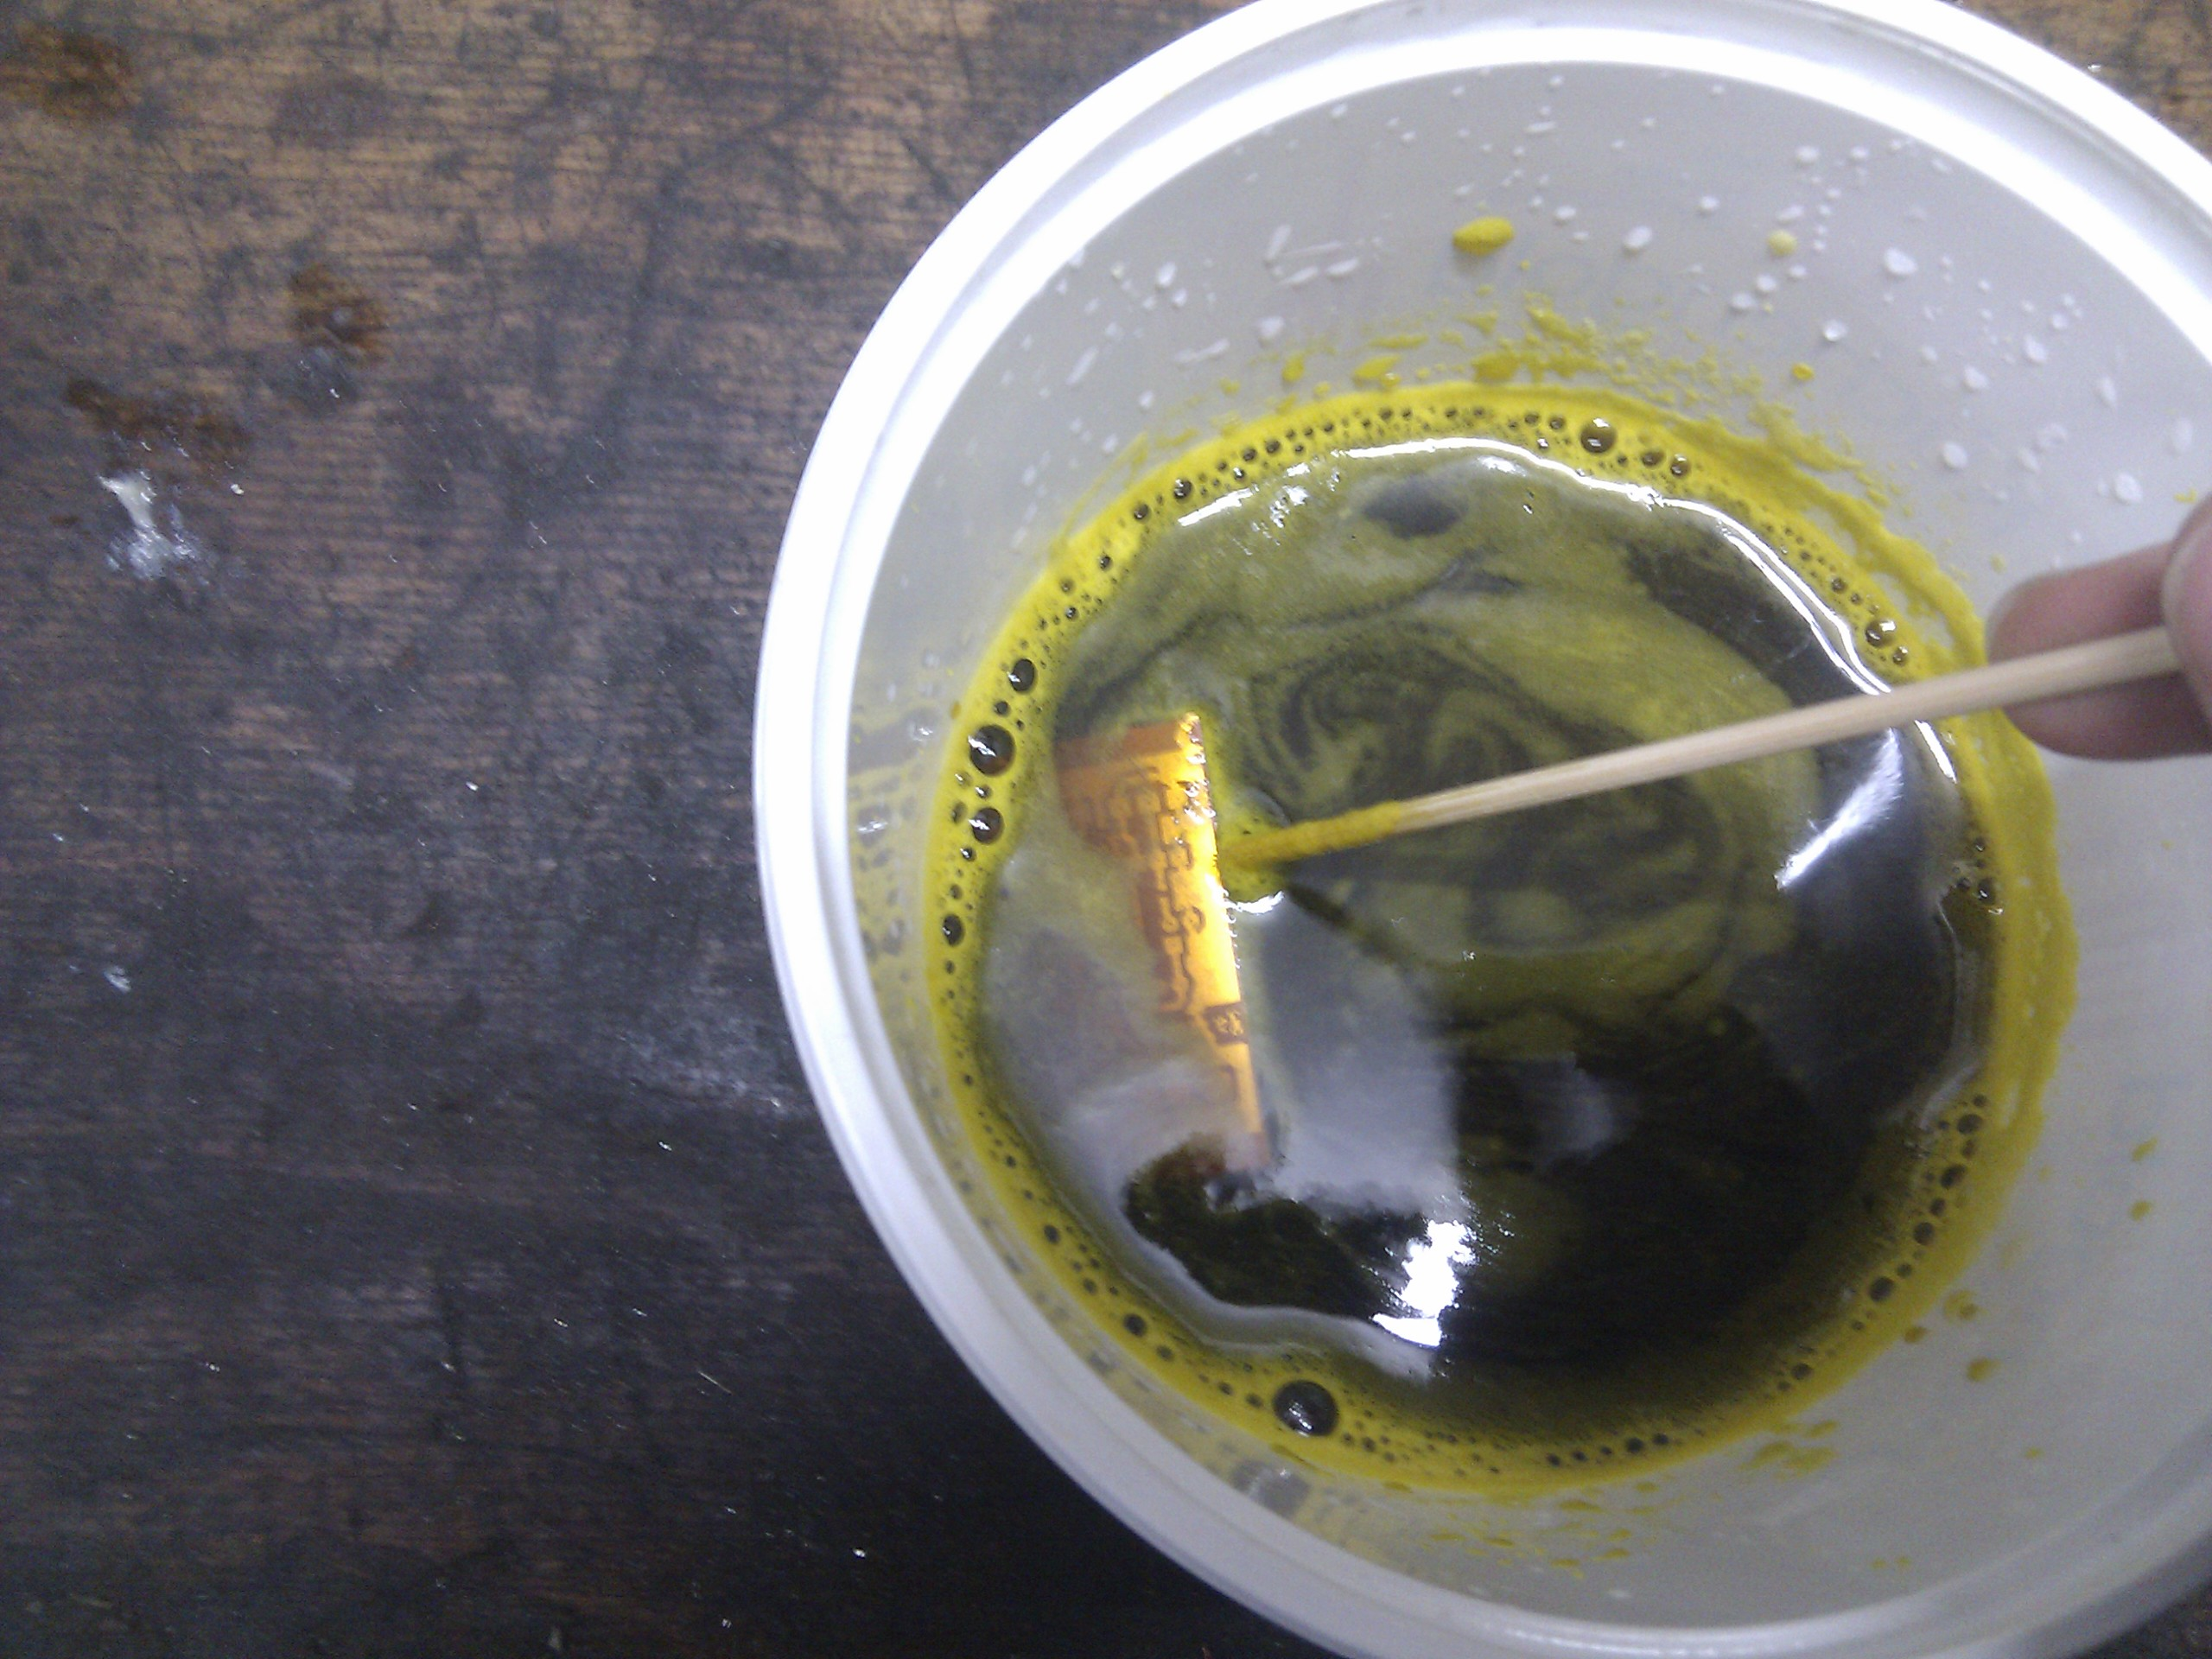
\includegraphics[width = \textwidth]{pics/raw/sensorboard_etch.jpg}
  \end{center}
\end{frame}
\subsection{Power Board}

\begin{frame}
  \frametitle{Powerboard}
  \begin{columns}
    \column{0.5\textwidth}
  \begin{center}
  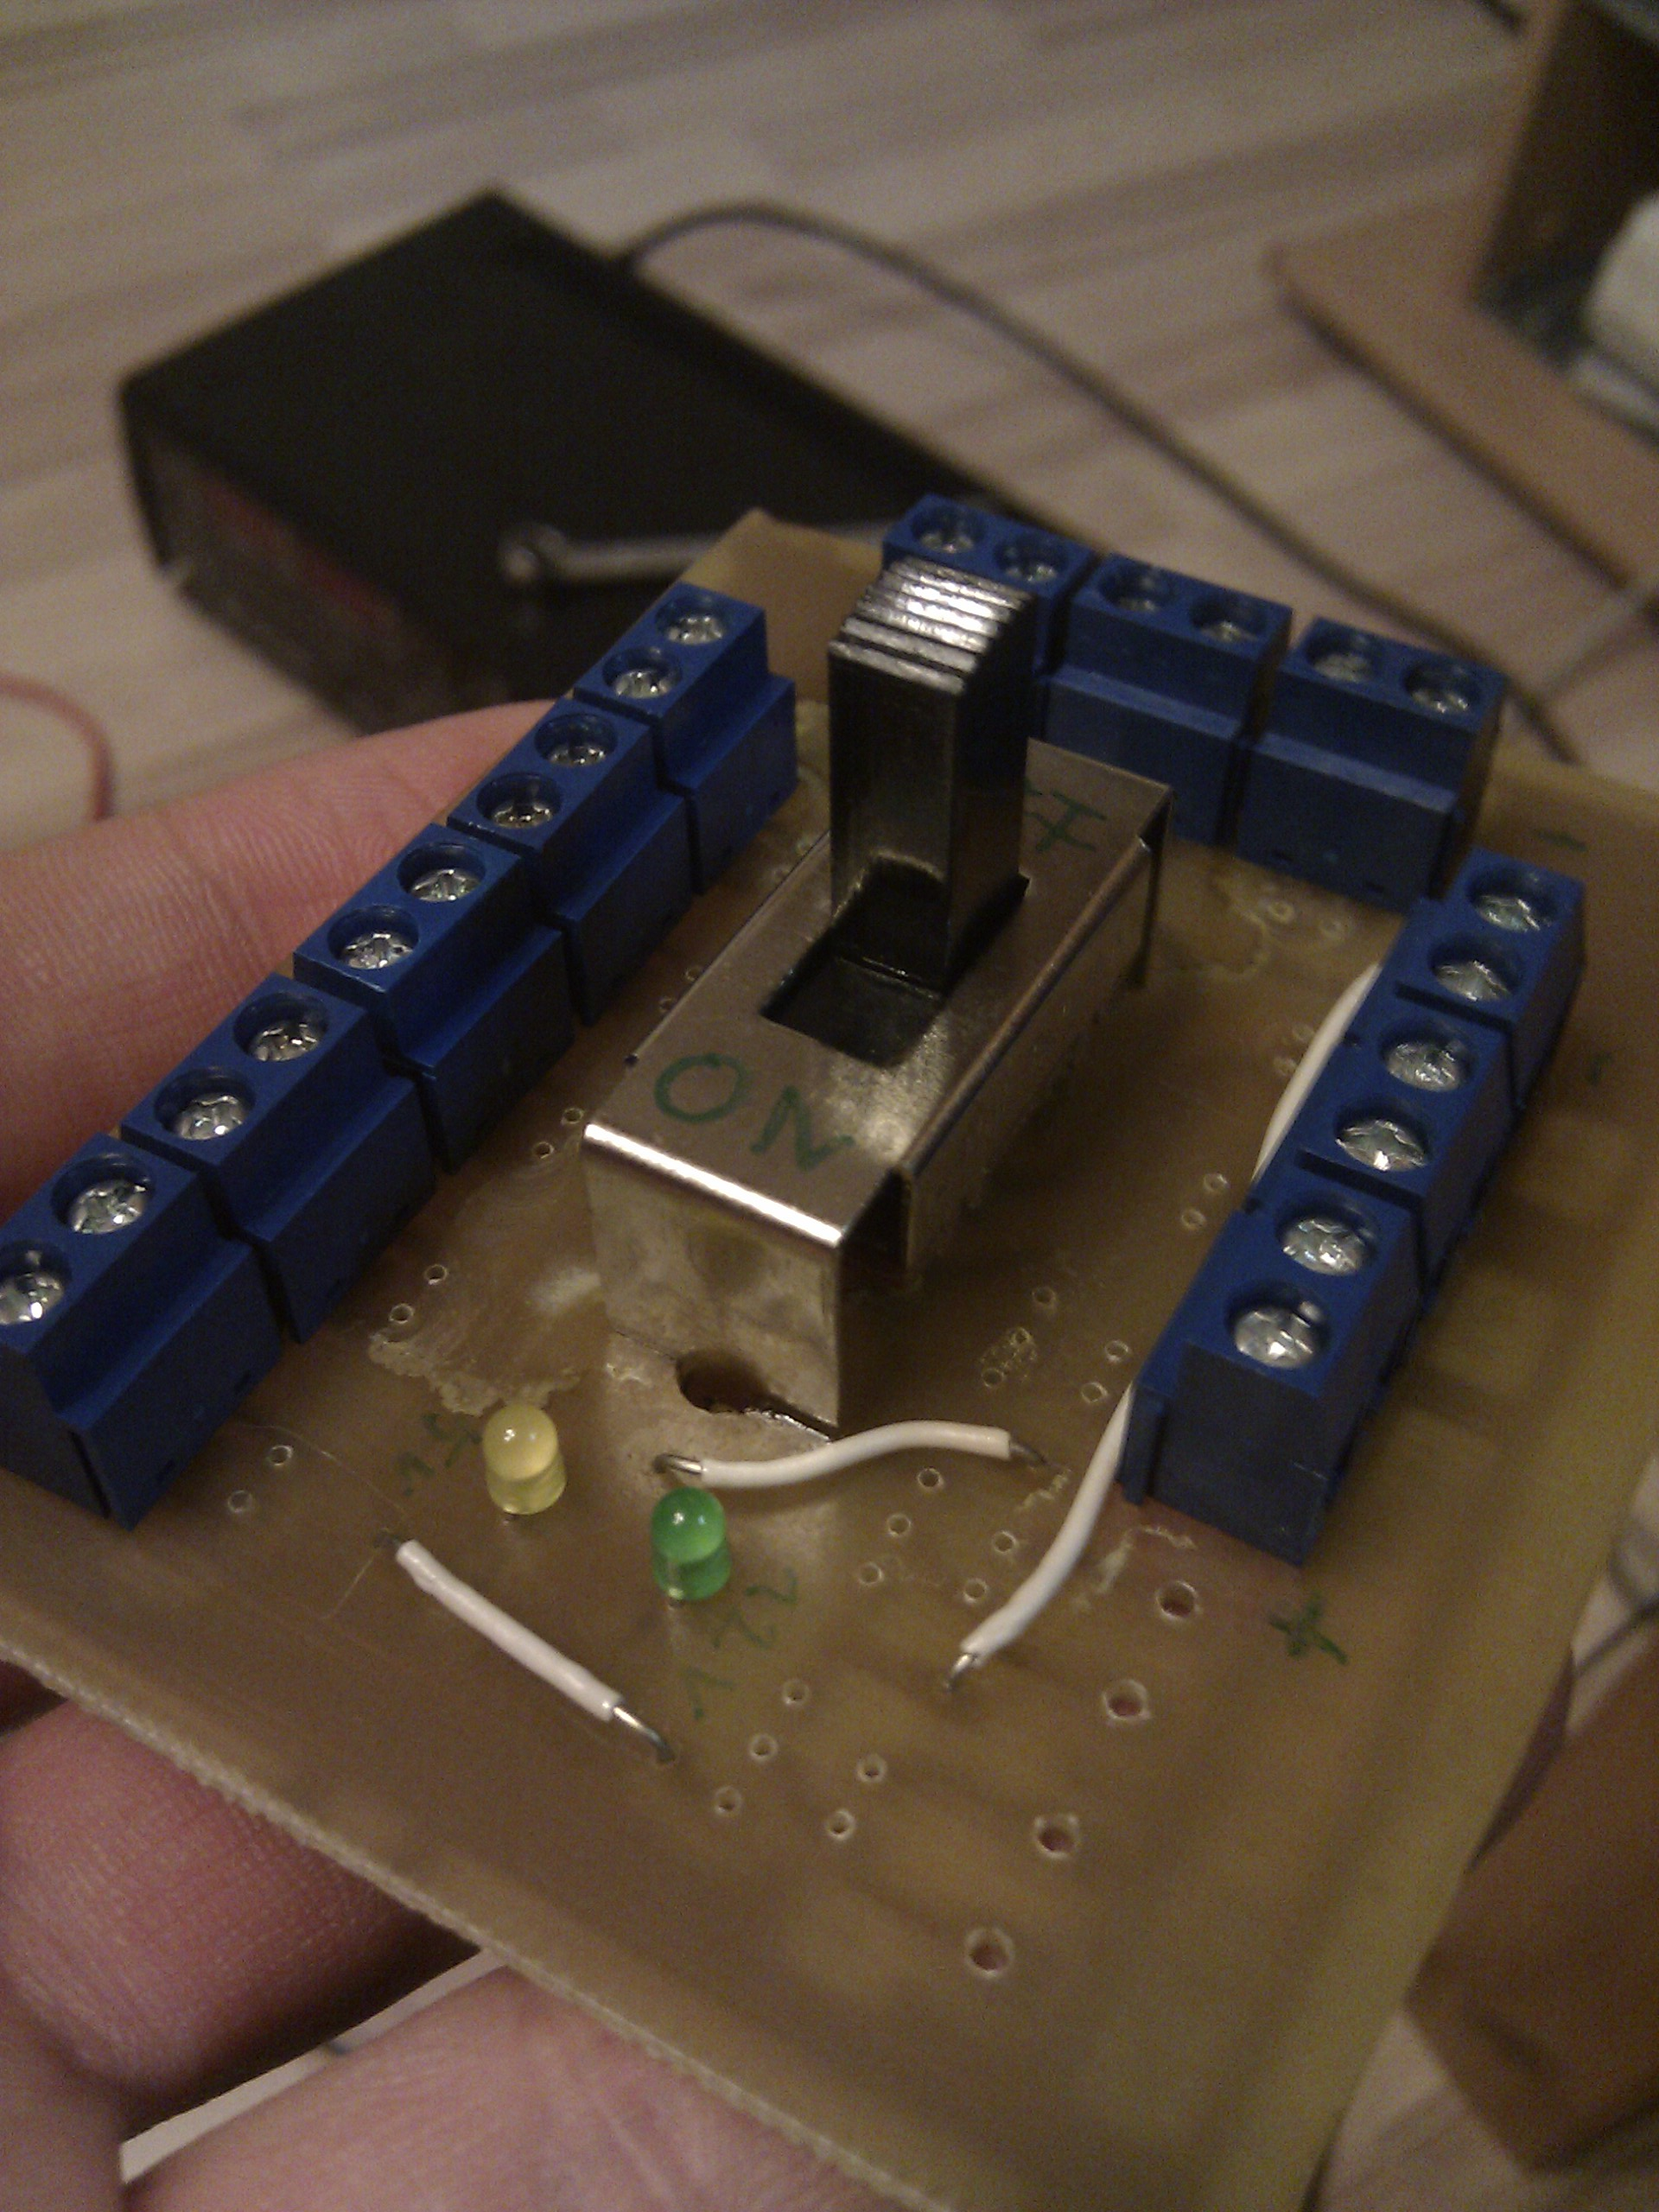
\includegraphics[width = 0.8\textwidth]{pics/raw/powerboard_1.jpg}
  \end{center}
    \column{0.5\textwidth}
  \begin{center}
  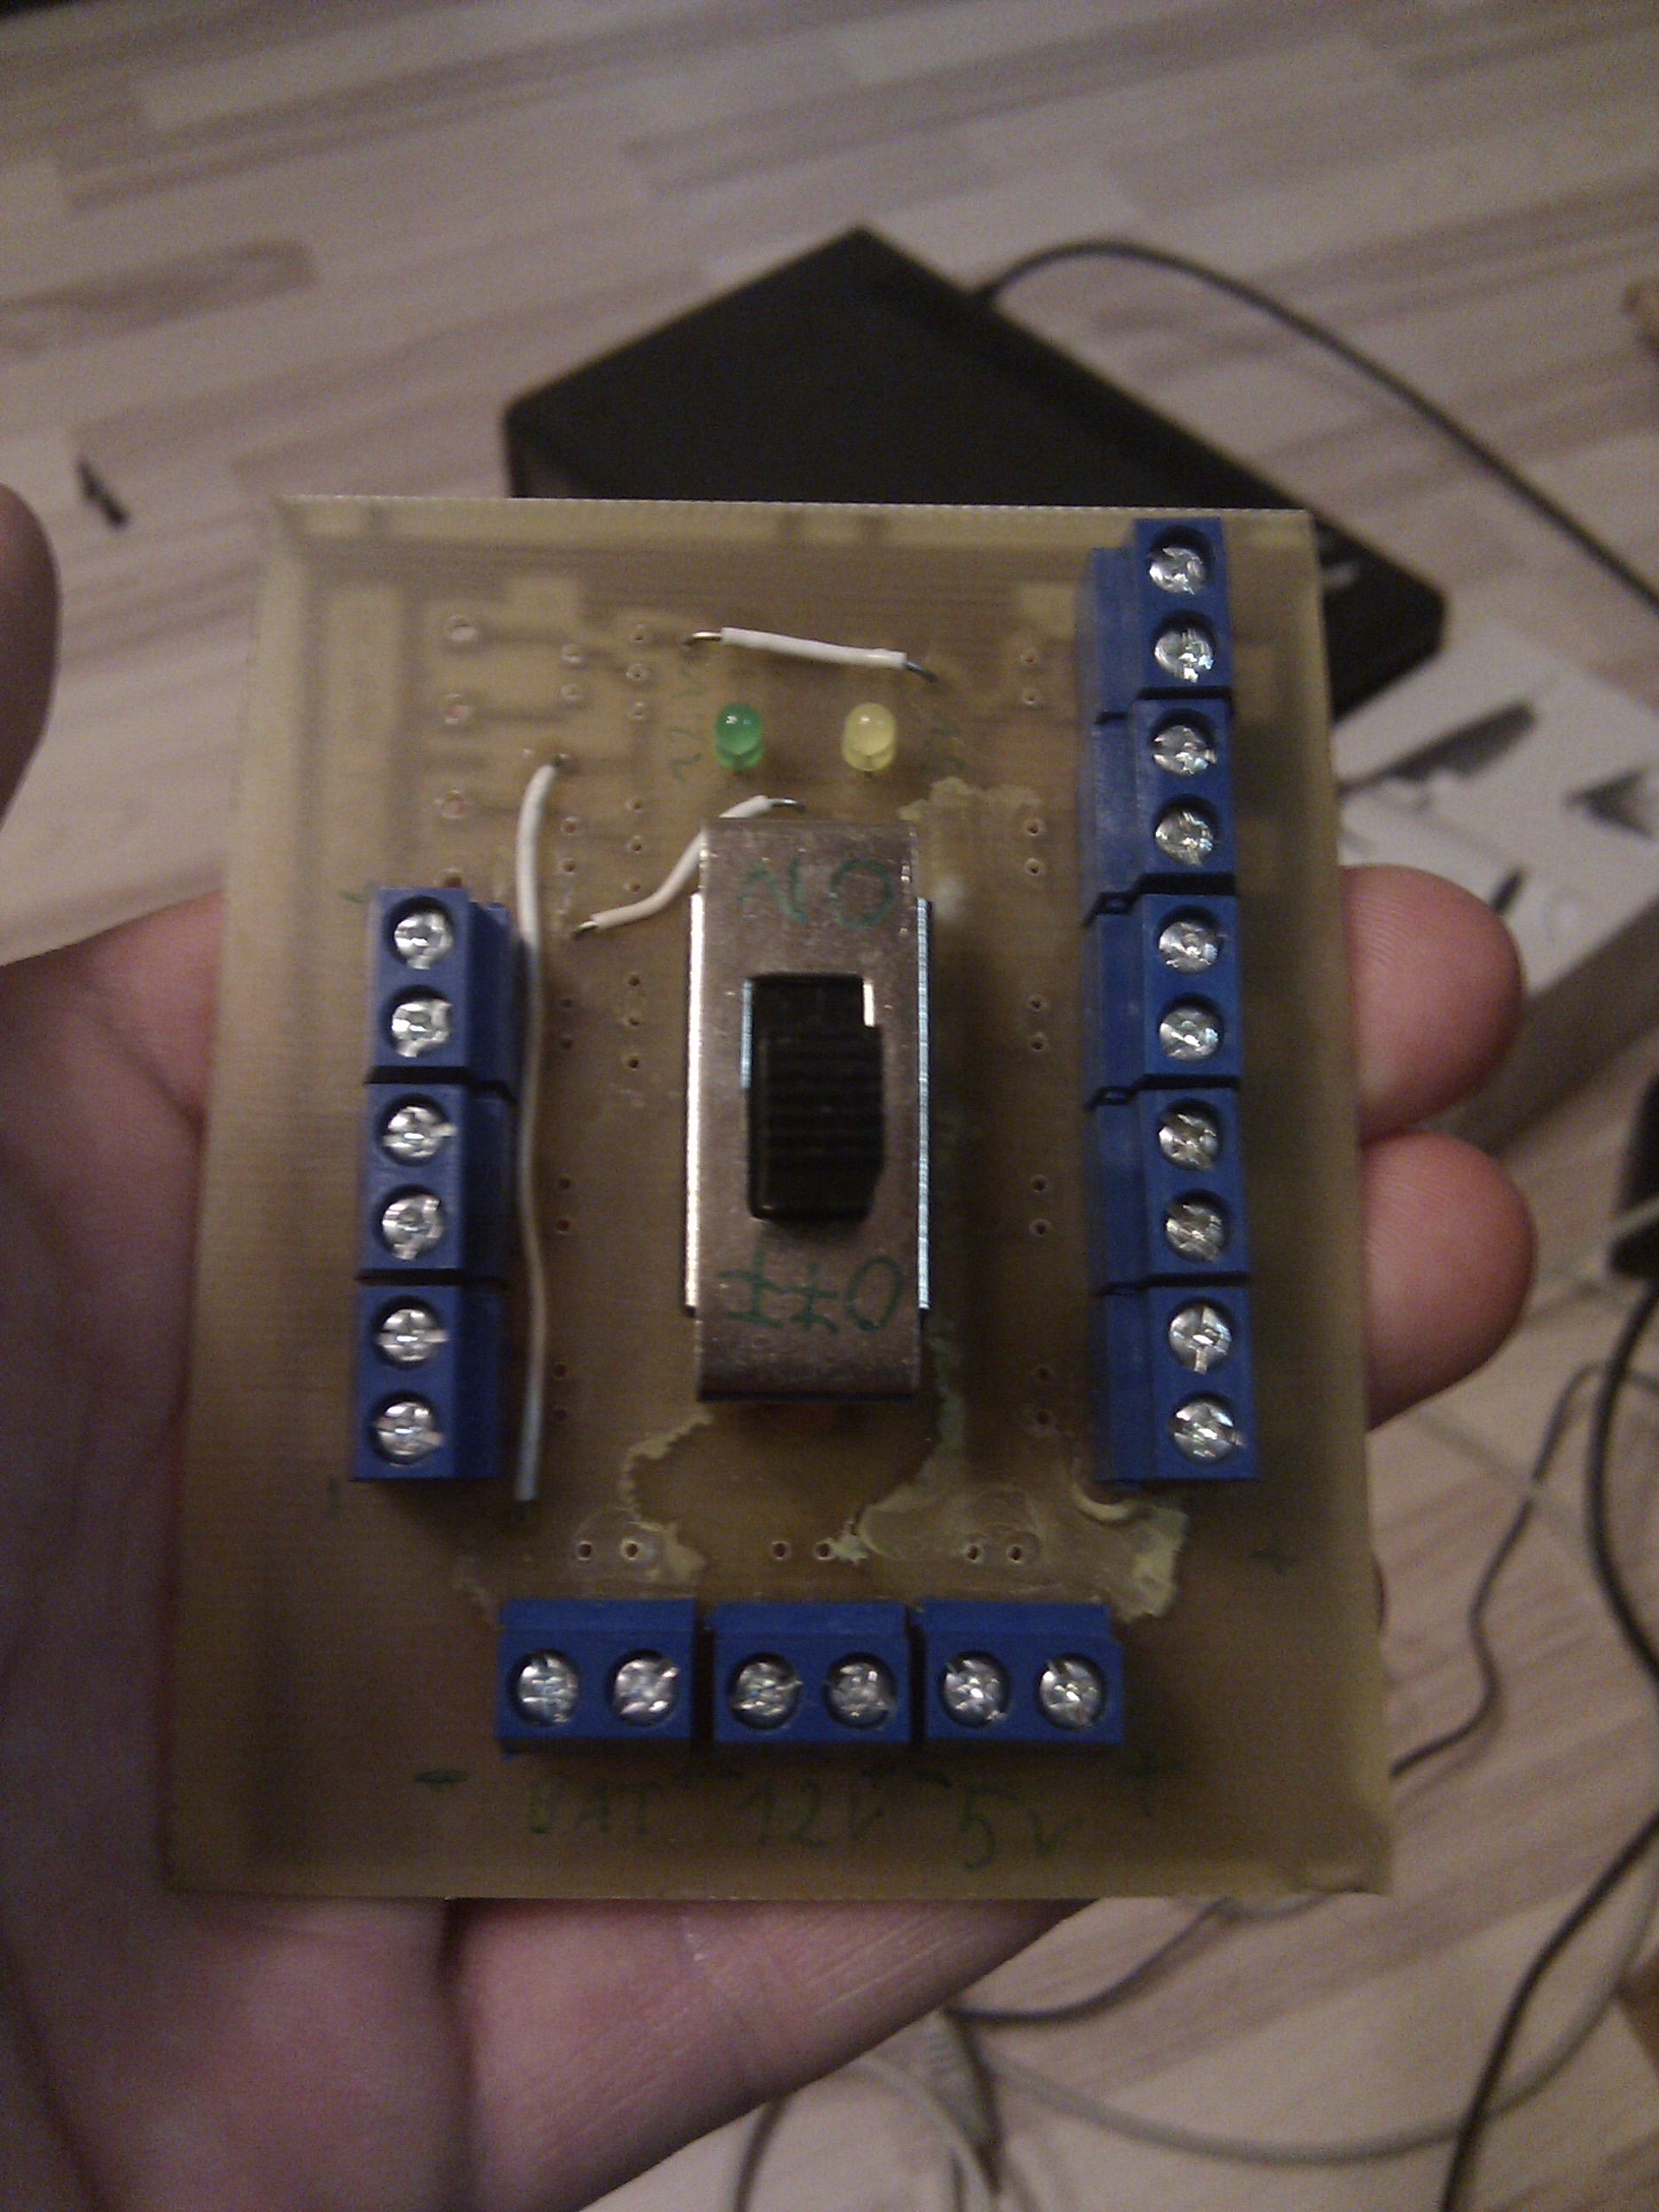
\includegraphics[width = 0.8\textwidth]{pics/raw/powerboard_2.jpg}
  \end{center}
  \end{columns}
\end{frame}


\subsection{Servoboard}

\begin{frame}
\frametitle{Servoboard}
  \begin{center}
  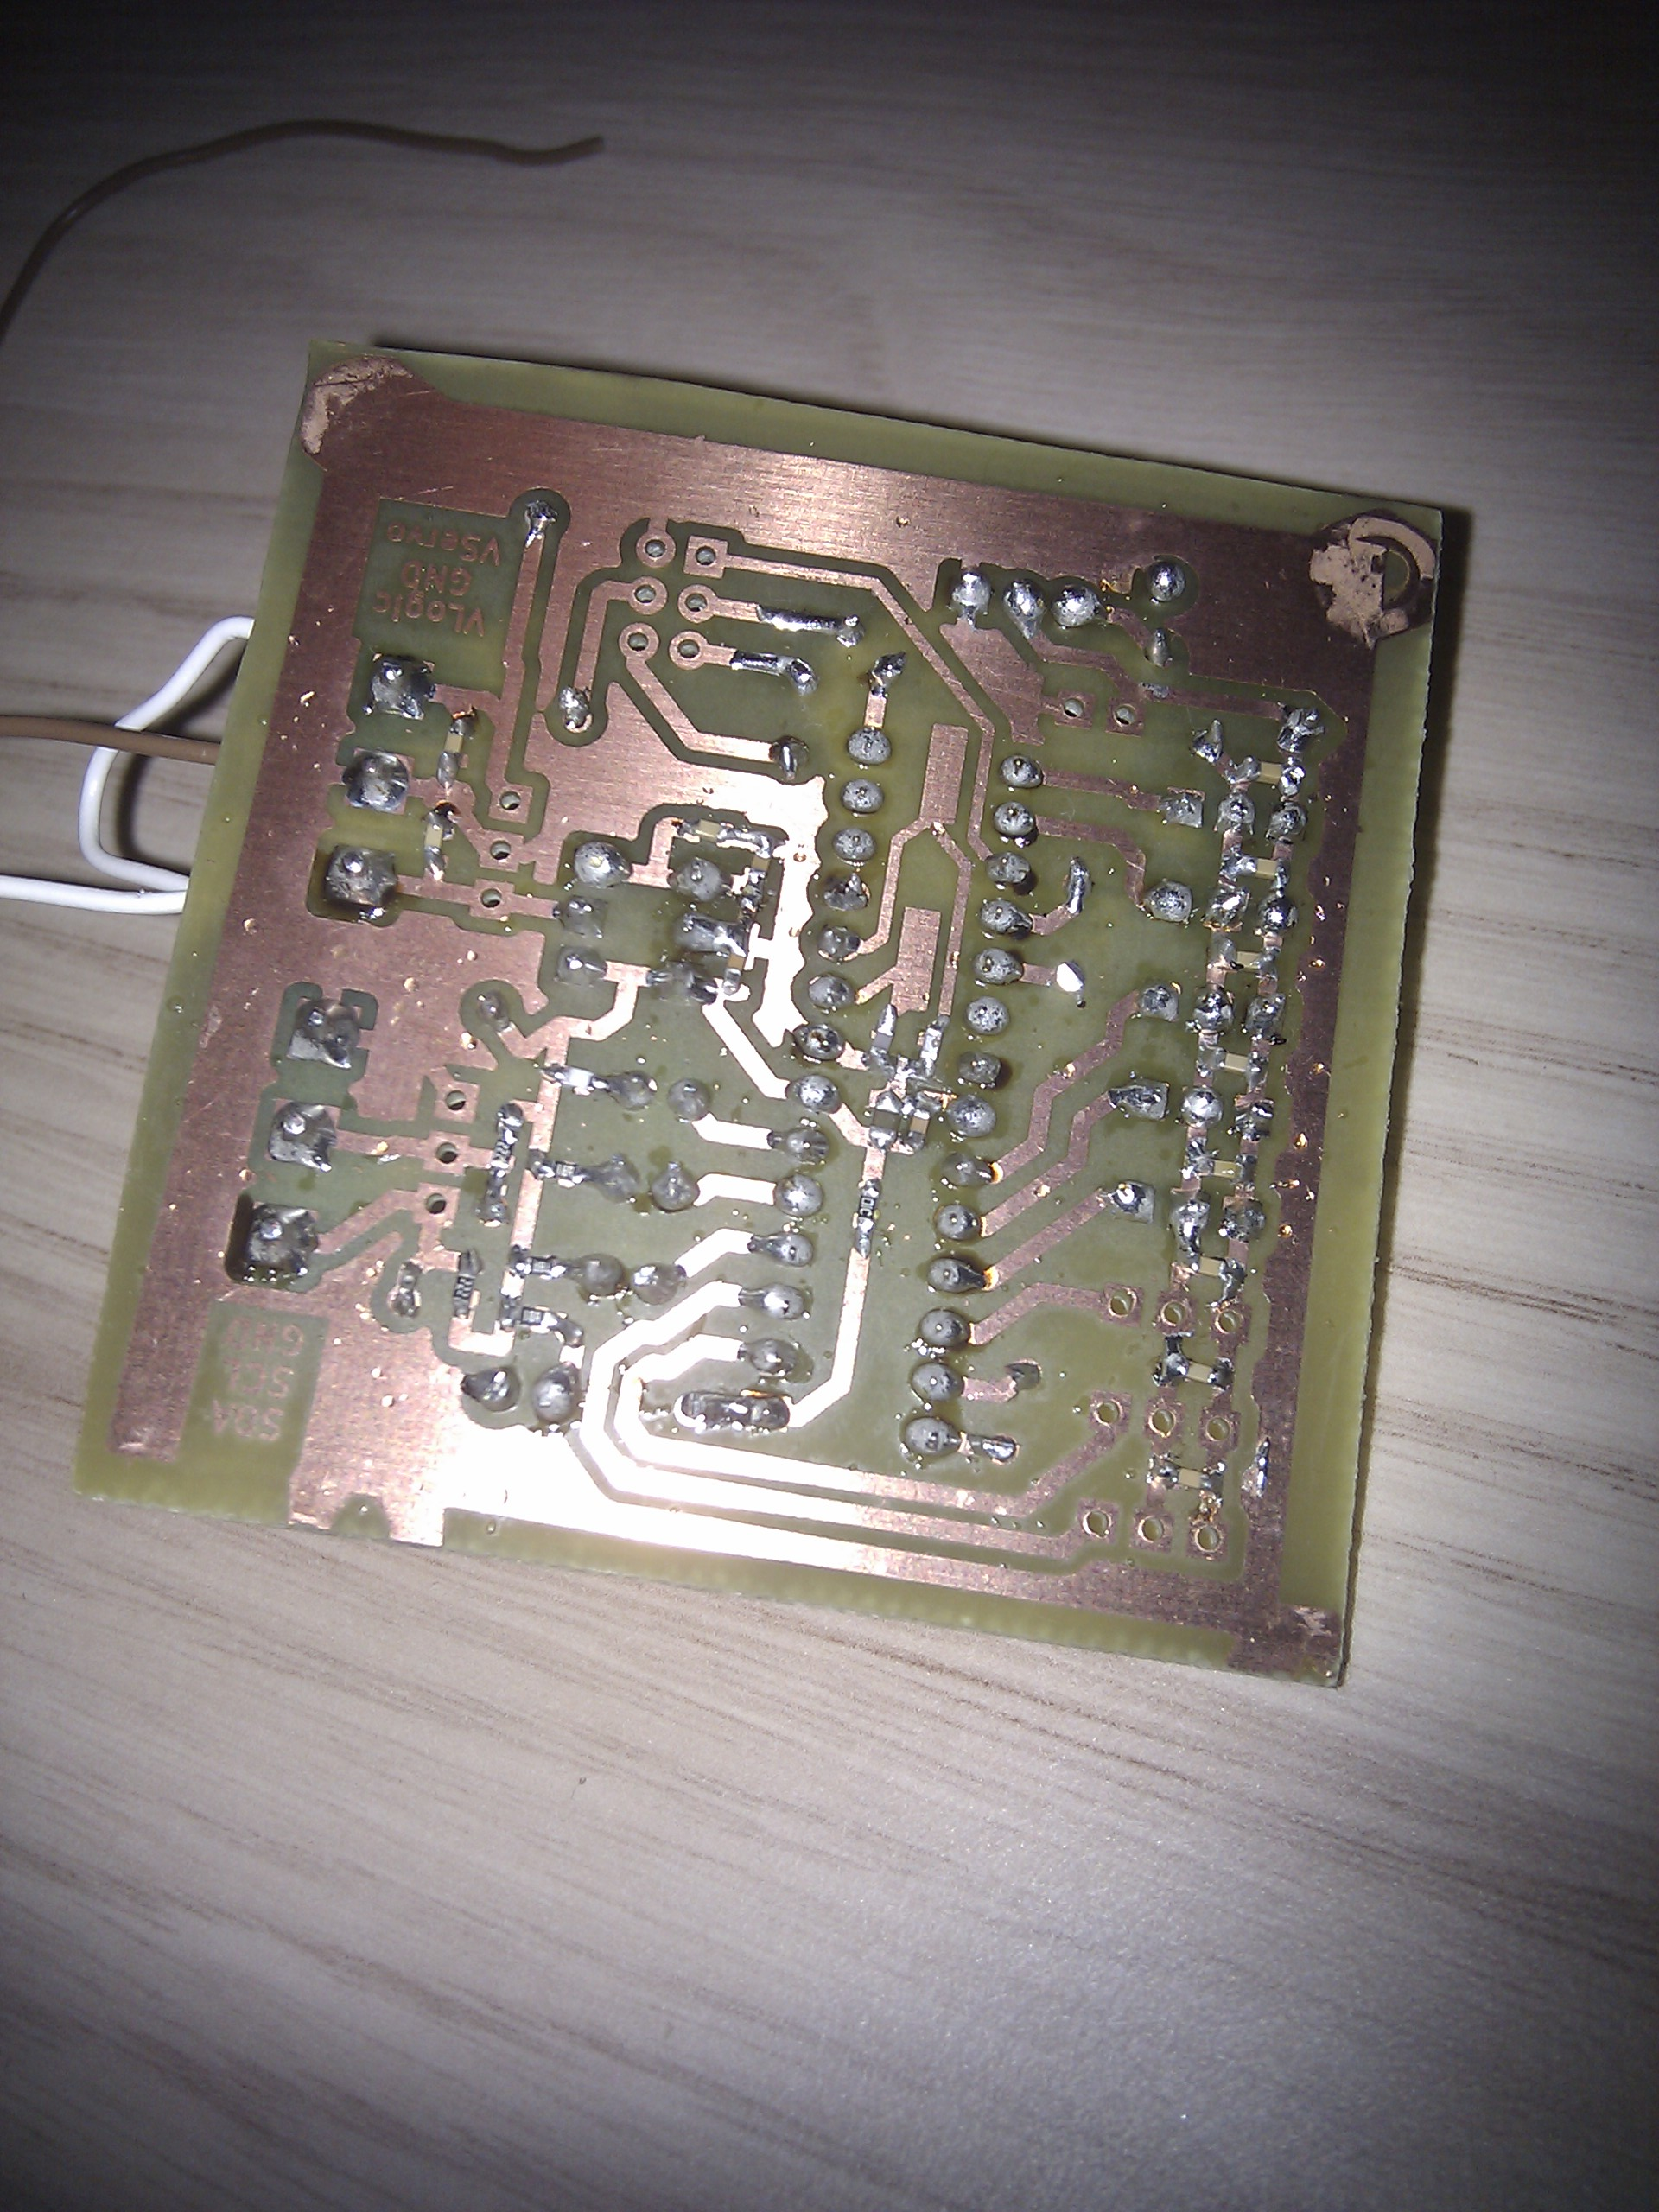
\includegraphics[width = 0.7\textwidth]{pics/raw/servoboard_rueckseite.jpg}
  \end{center}
\end{frame}

\begin{frame}
  \begin{center}
  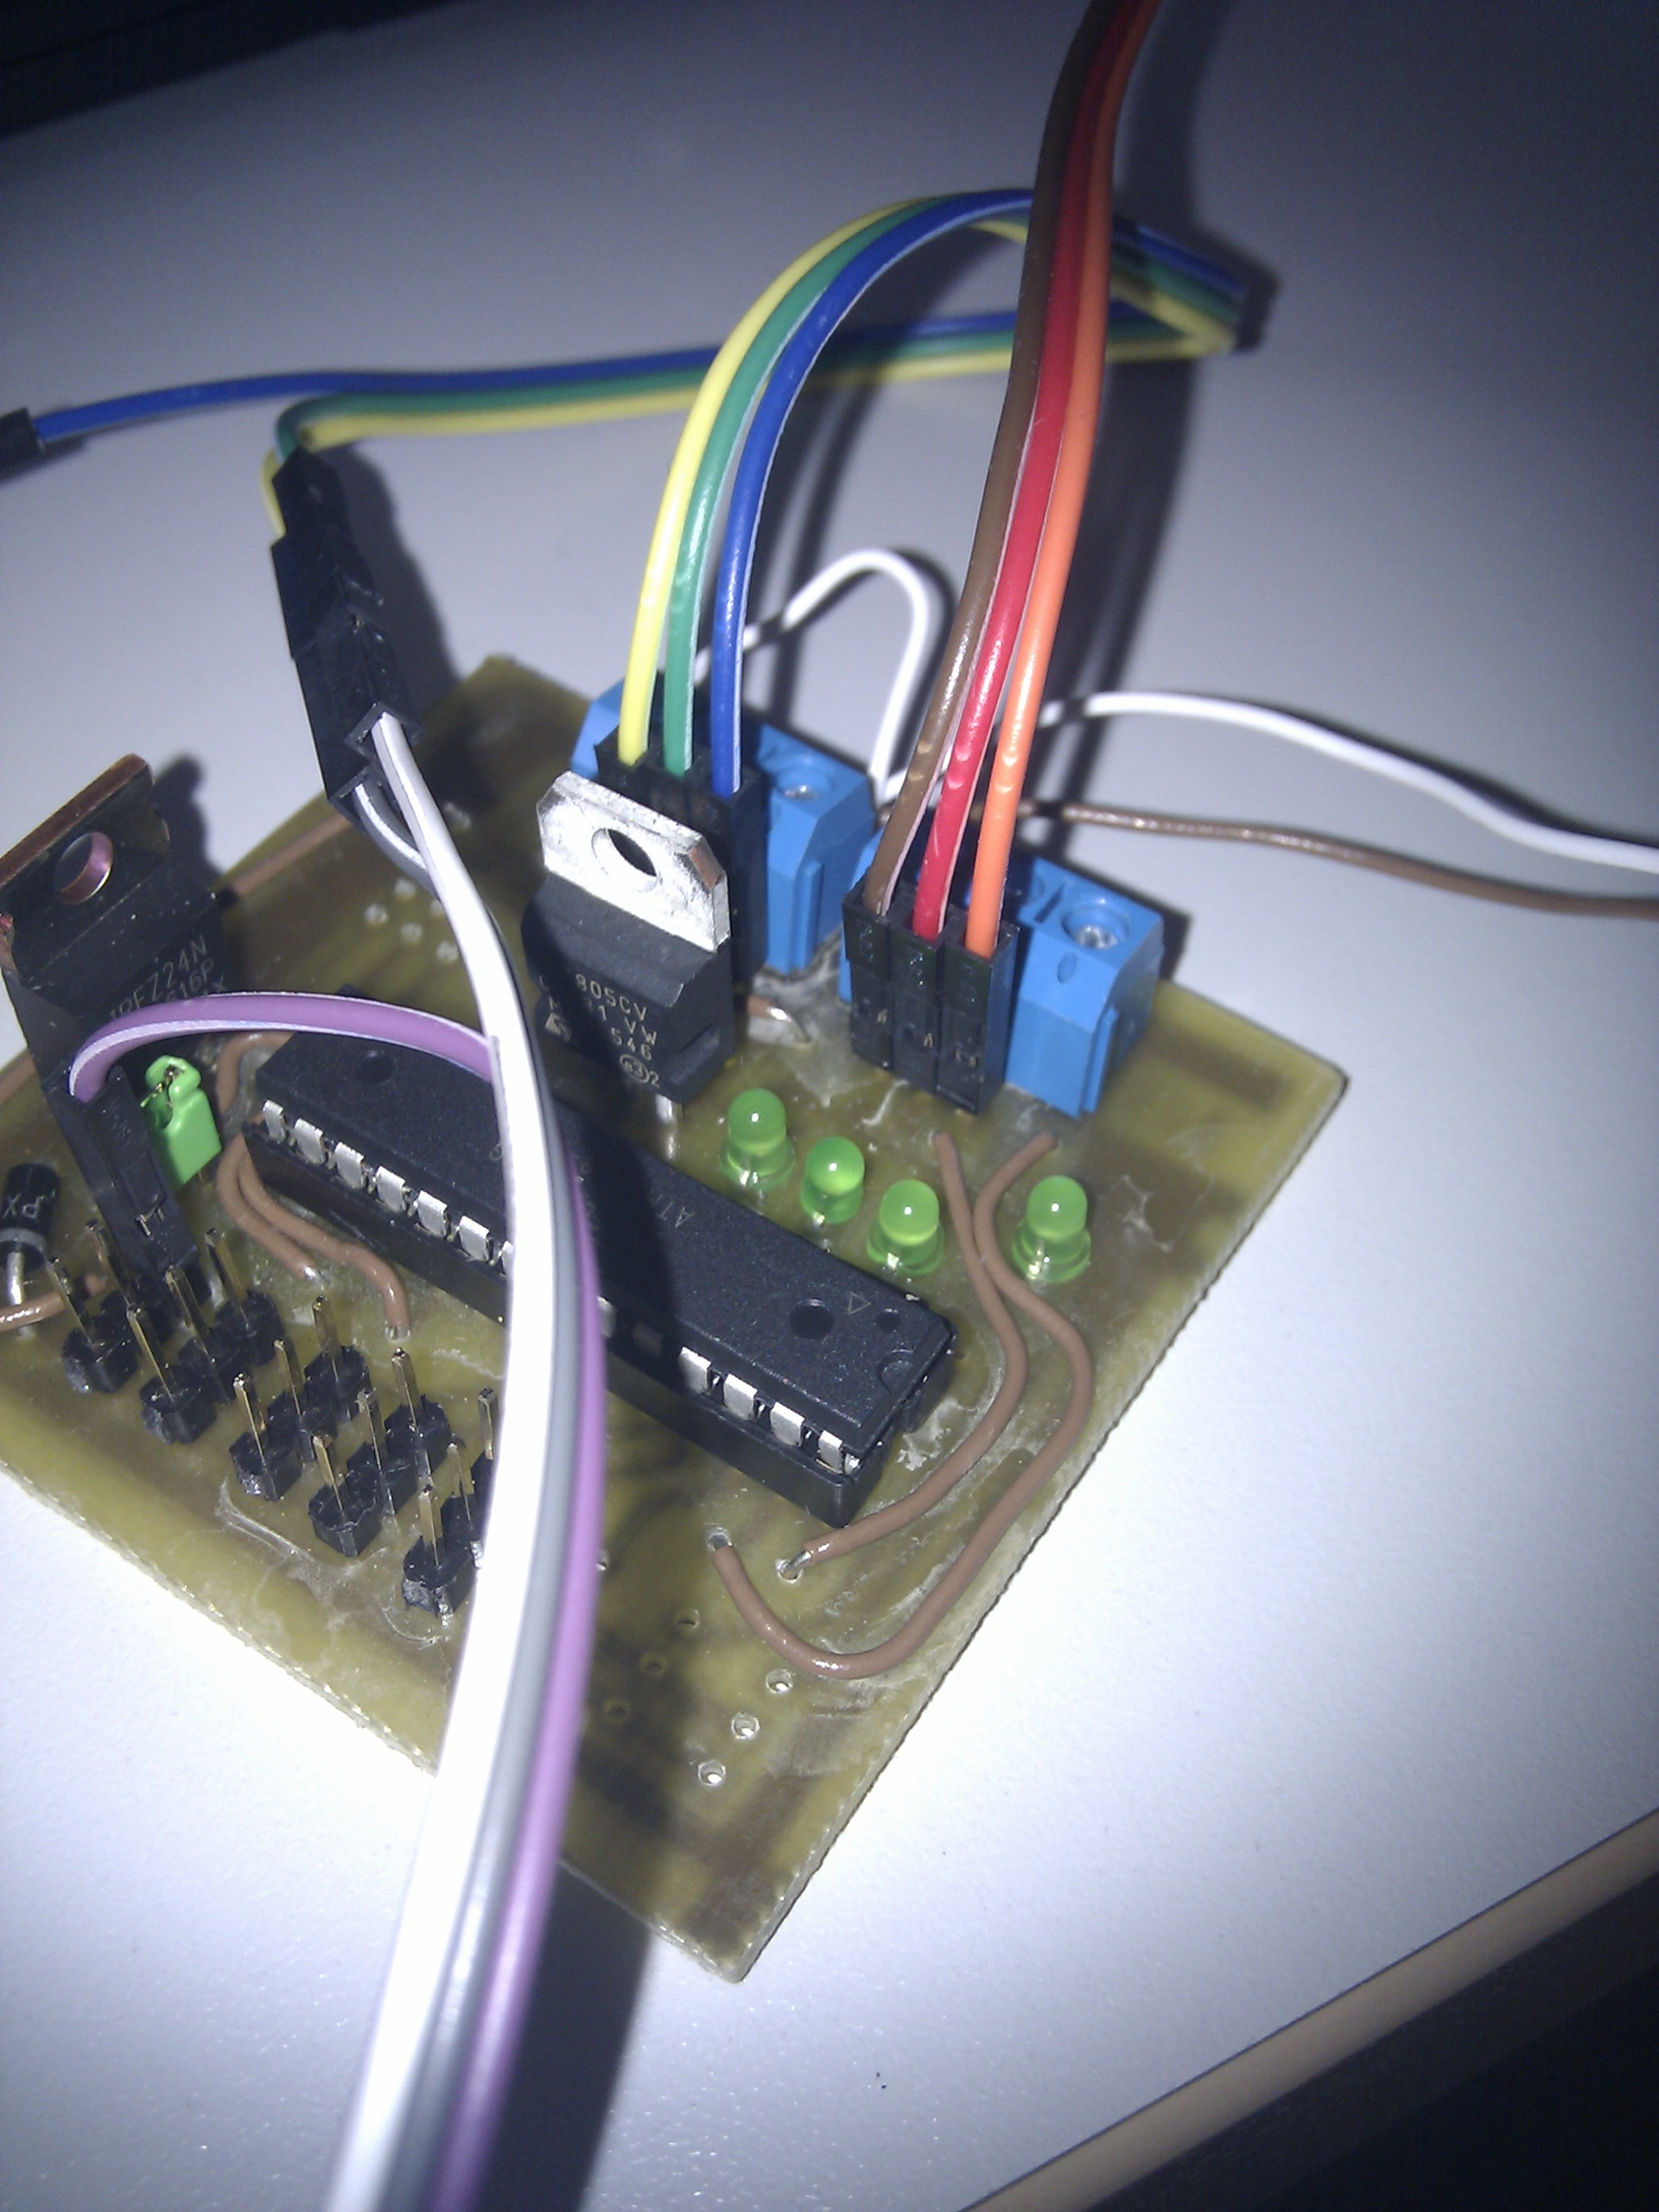
\includegraphics[width = 0.7\textwidth]{pics/raw/servoboard_firsttest.jpg}
  \end{center}
\end{frame}
\begin{frame}
\frametitle{Servoboard}
\begin{exampleblock}{Features}
\begin{itemize}
  \item Controls up to 8 servos or motor drivers
  \item 13 Bit resolution per servo
  \item Communication via I2C
  \item Emergency shutdown
  \item Separate servo supply voltage possible
\end{itemize}
\end{exampleblock}
\end{frame}
\begin{frame}
\frametitle{Demo/Video}
  \begin{center}
  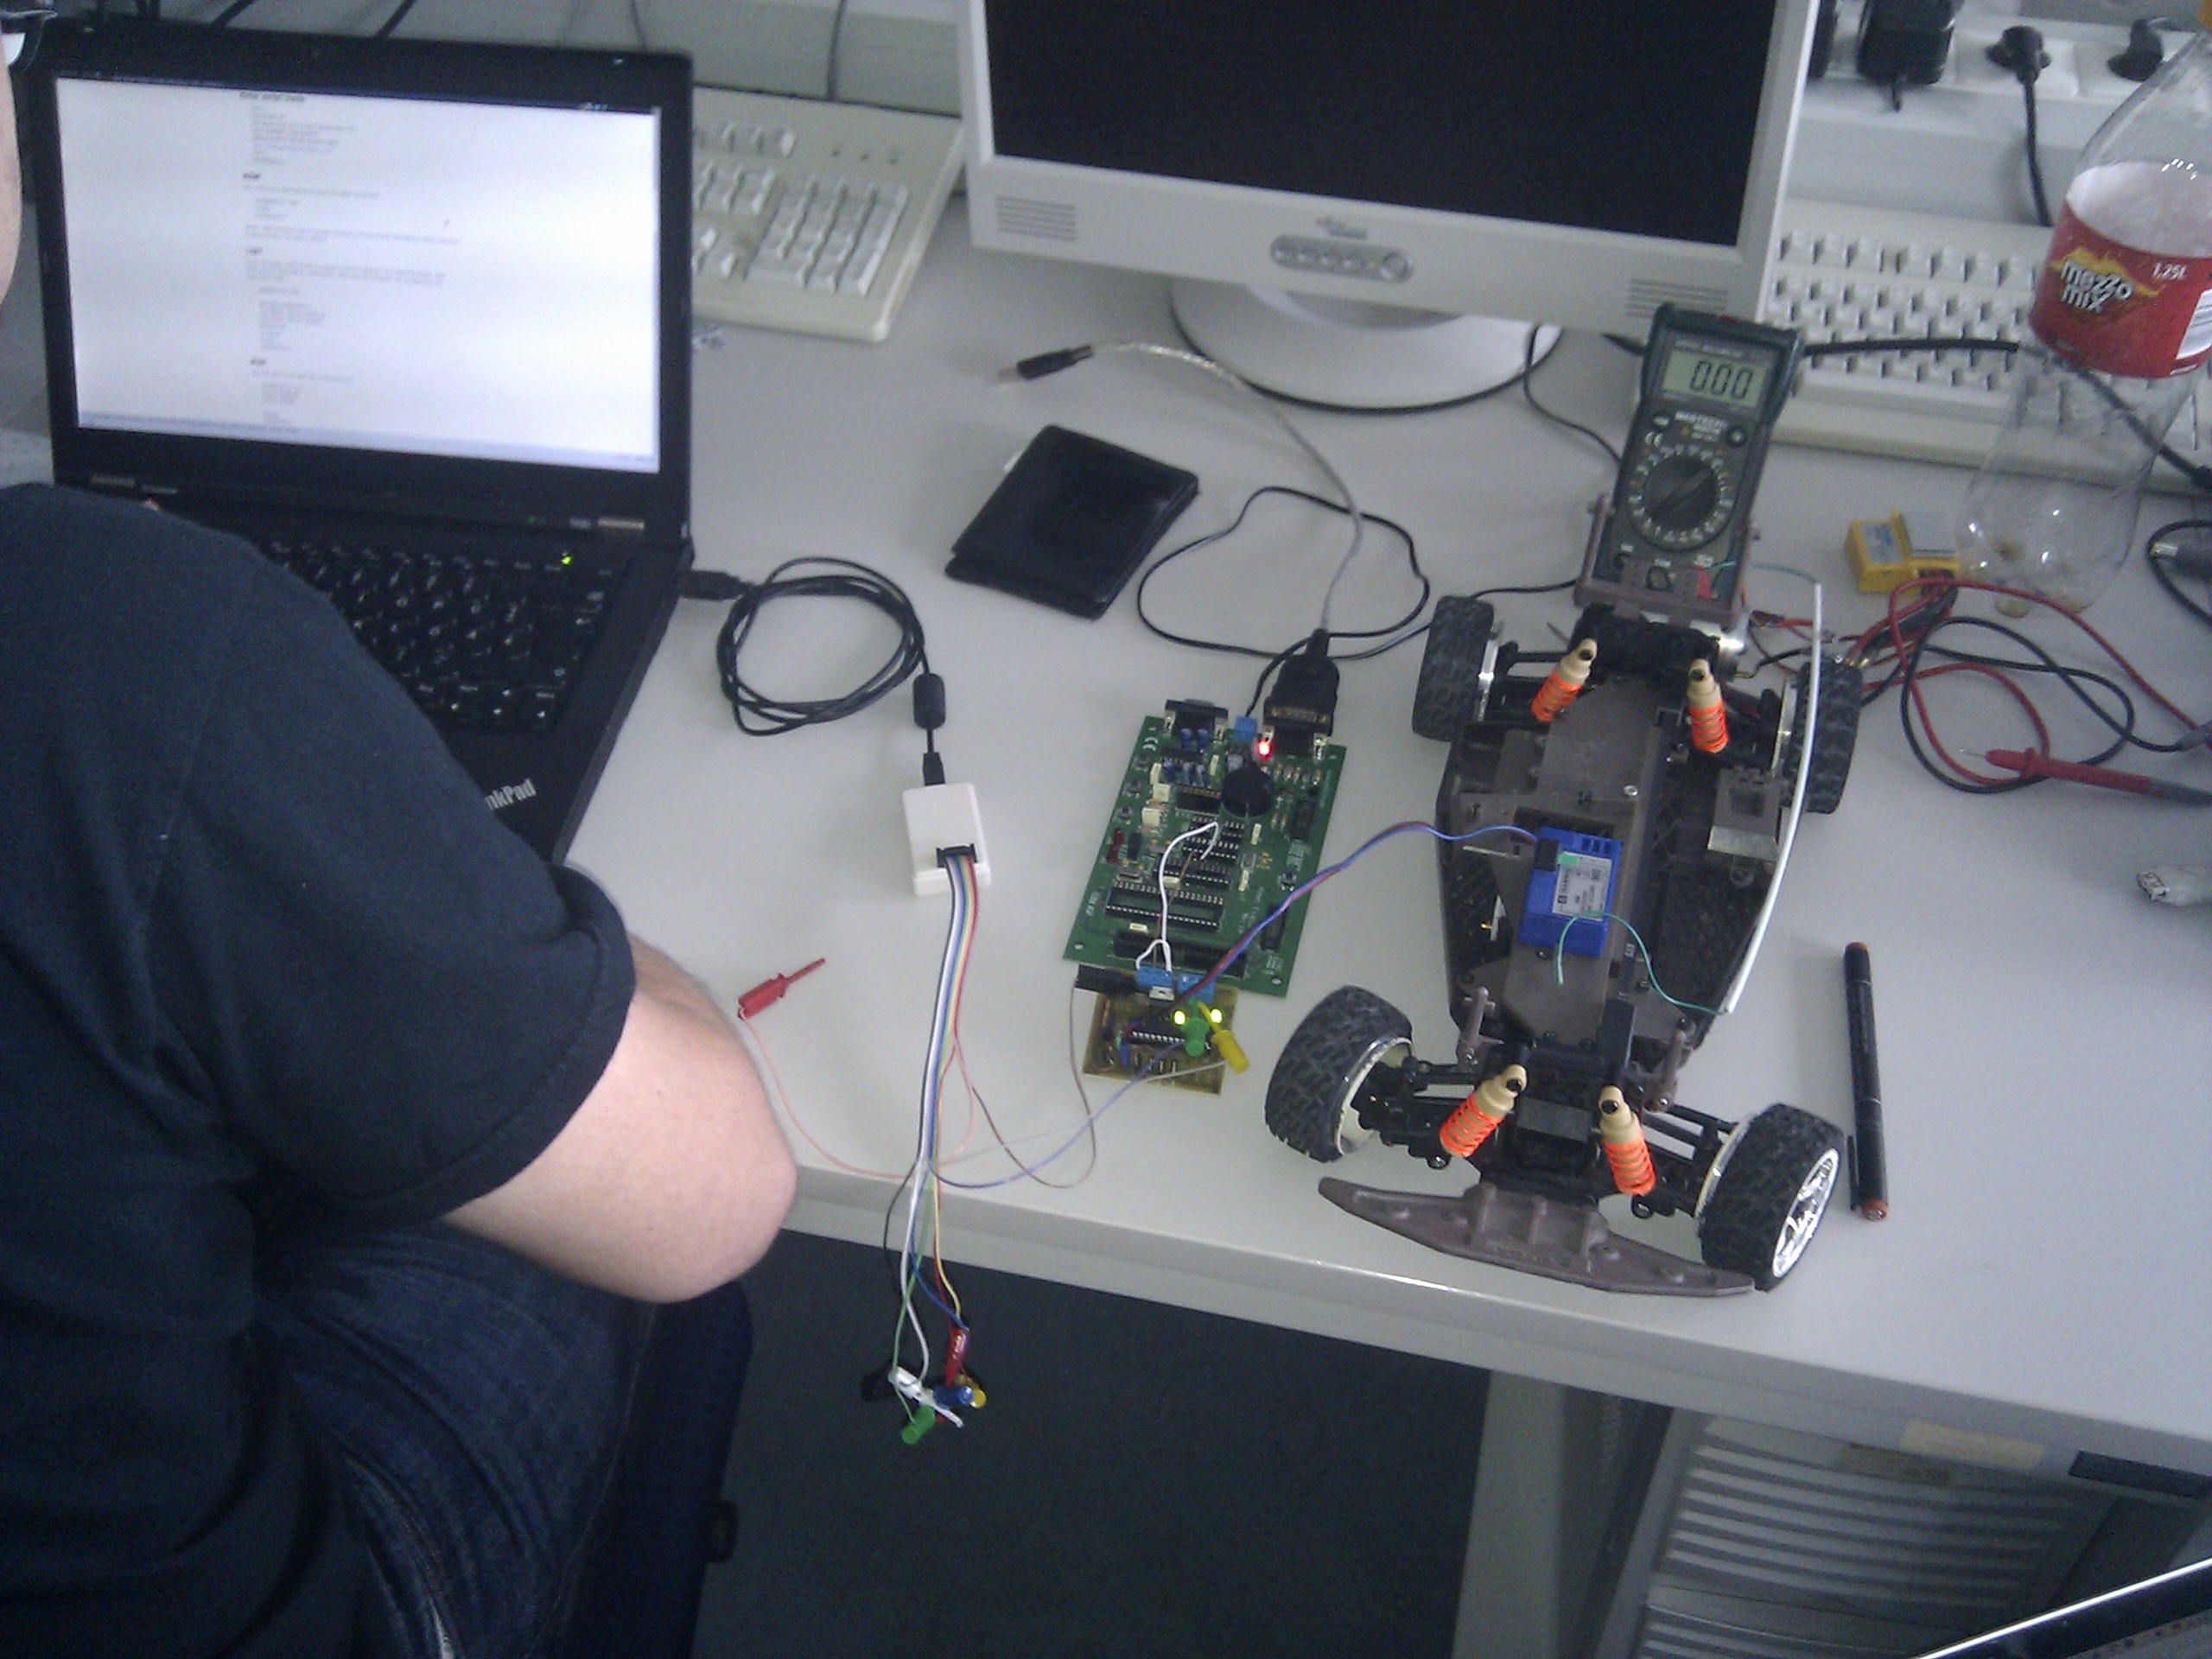
\includegraphics[width = \textwidth]{pics/raw/servoboard_test2.jpg}
  \end{center}
\end{frame}

\section{Hardware}
\subsection{Encoder}
\begin{frame}
Problem: Tests at MI building $\Rightarrow$ Back wheels of Car are sliding most of the time
\begin{exampleblock}{IDEA: Traction Control System}
\begin{itemize}
  \item Measure speed at front AND back wheels
  \item[$\rightarrow$] Compare!
  \item Adjust motor according to speed difference
\end{itemize}
\end{exampleblock}
\end{frame}

\begin{frame}
  \begin{columns}
    \column{0.5\textwidth}
      \begin{center}
      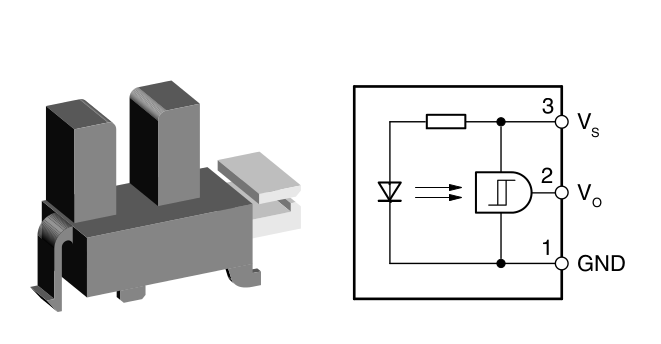
\includegraphics[width = 1.0\textwidth]{pics/raw/ls.png}
      \end{center}
    \column{0.5\textwidth}
      \begin{center}
      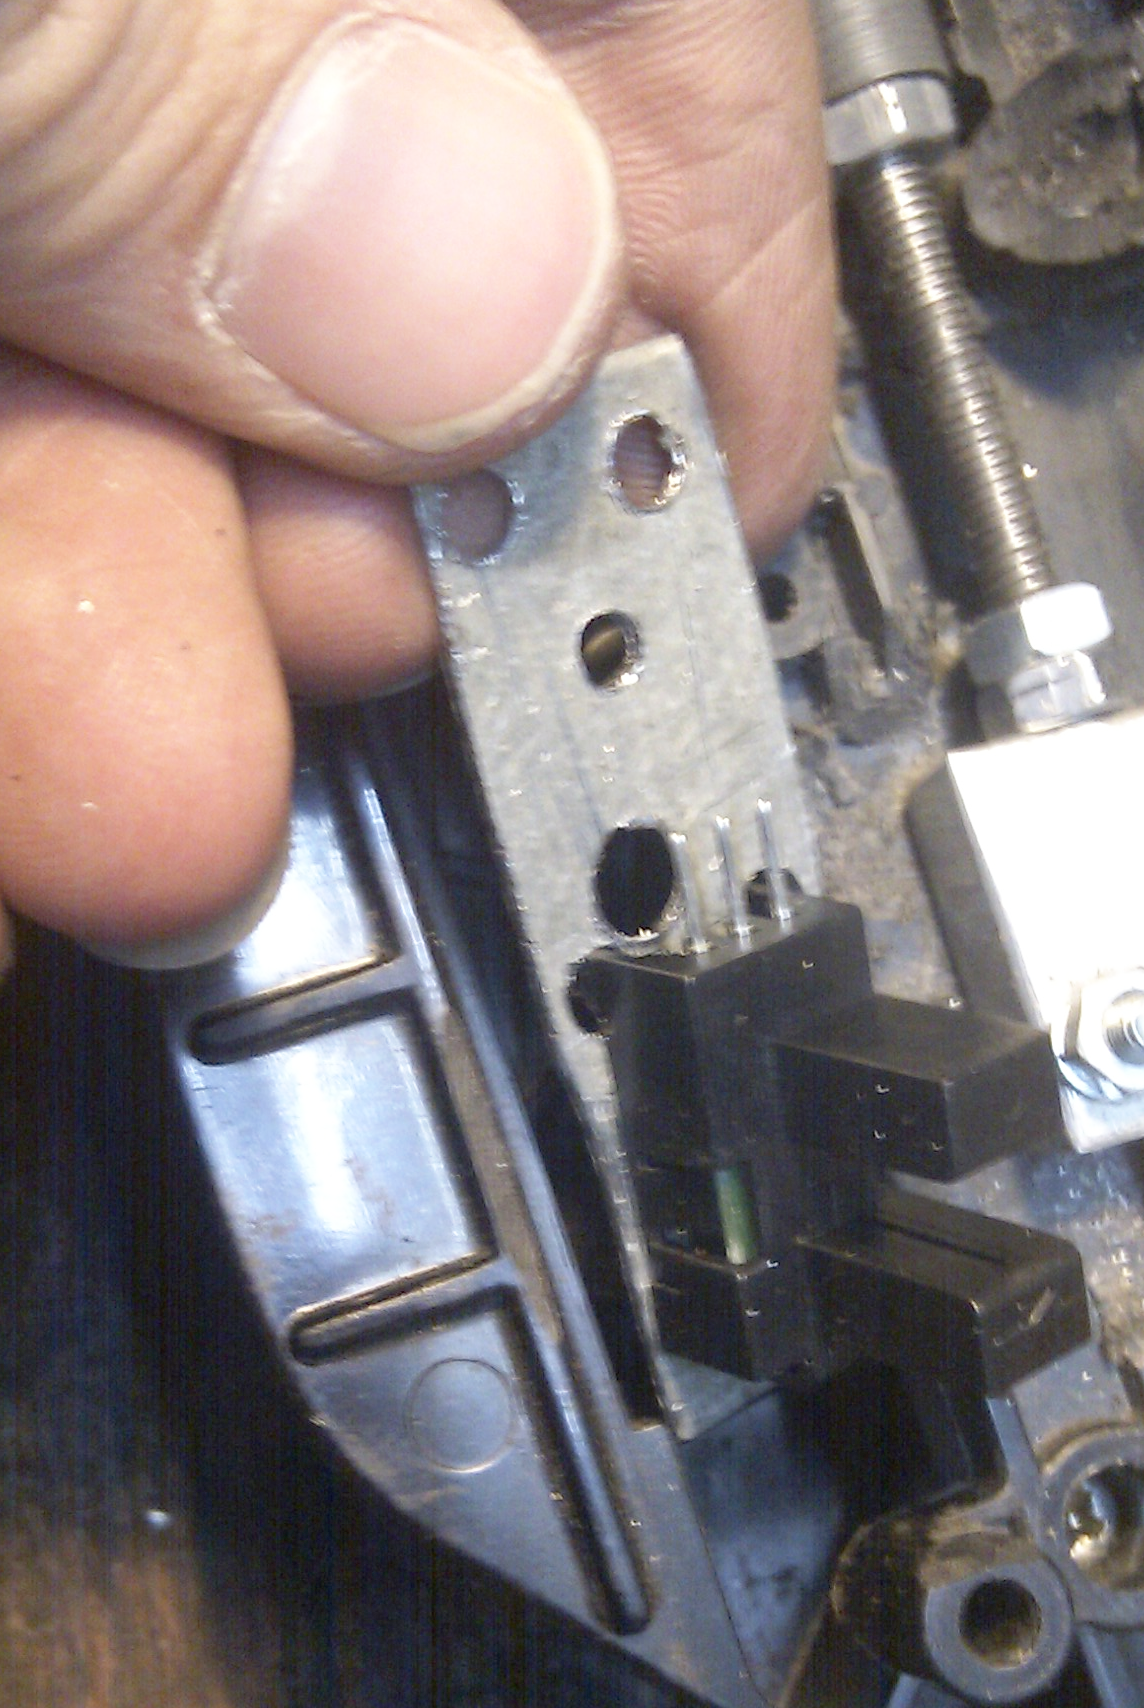
\includegraphics[width = 0.8\textwidth]{pics/raw/encoder_blech.png}
      \end{center}
  \end{columns}
\end{frame}

\begin{frame}
  \begin{center}
  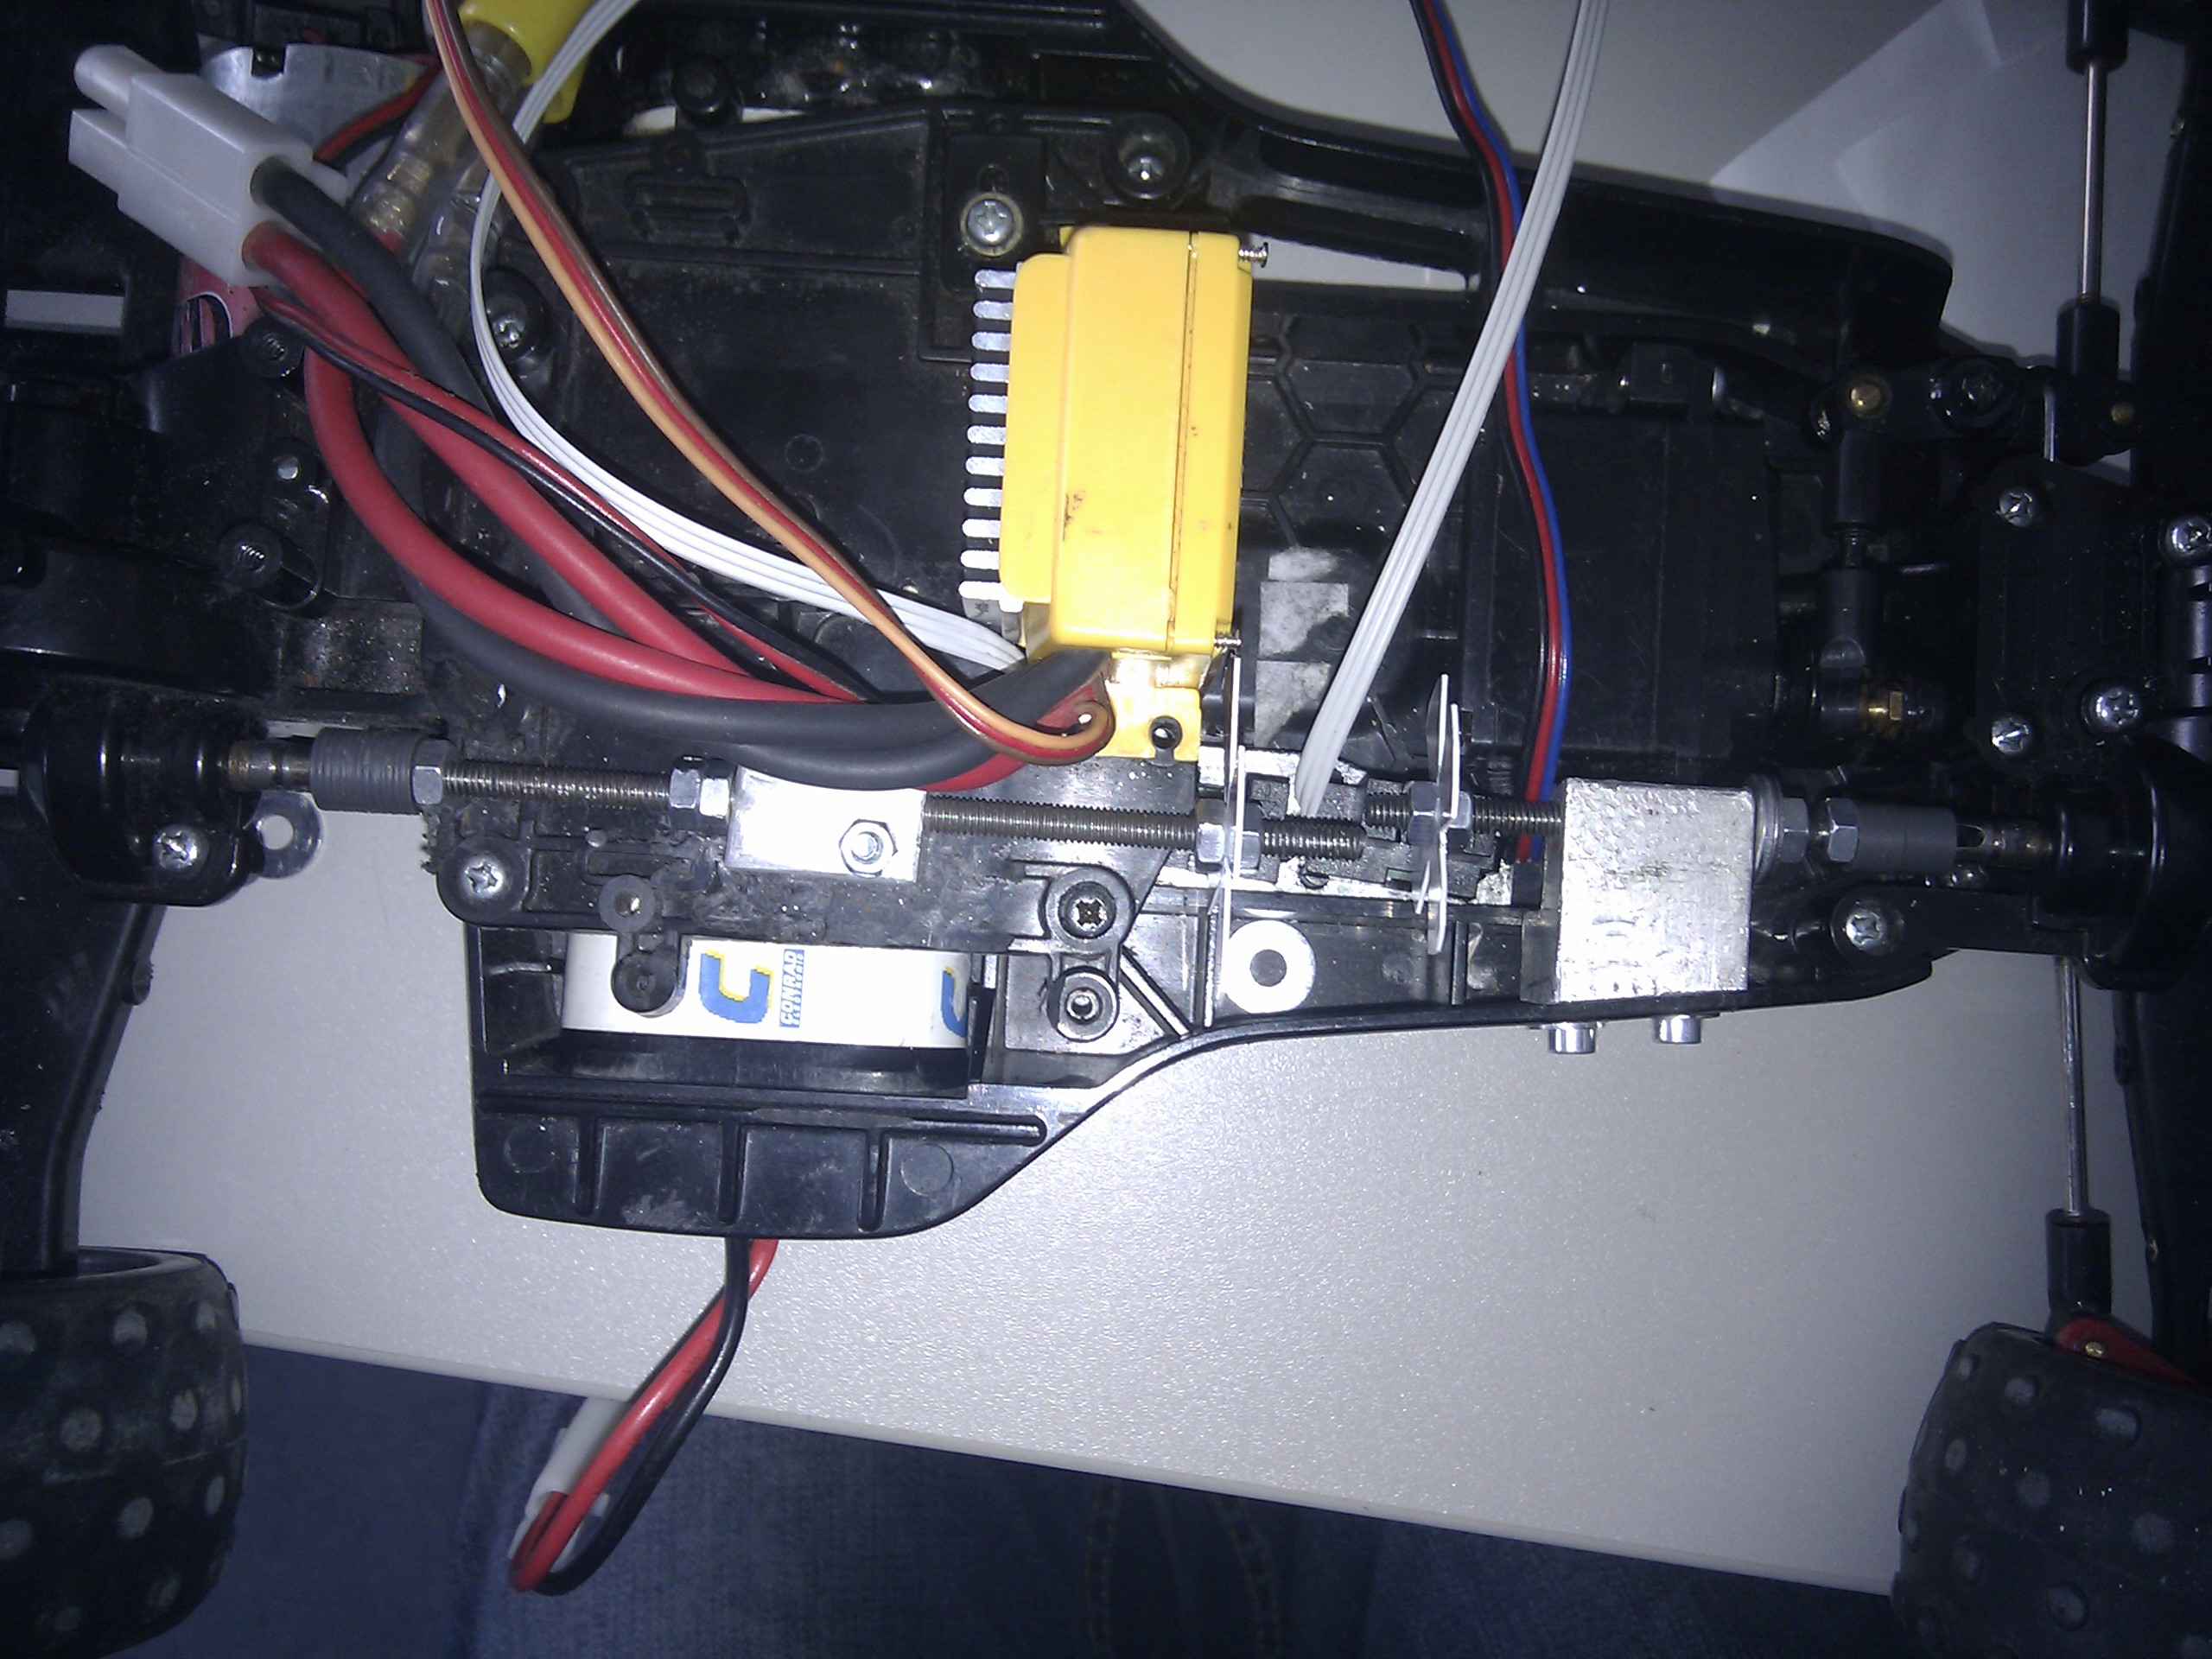
\includegraphics[width = \textwidth]{pics/raw/encoders_top.png}
  \end{center}
\end{frame}
\begin{frame}
  \begin{columns}
    \column{0.5\textwidth}
  \begin{center}
  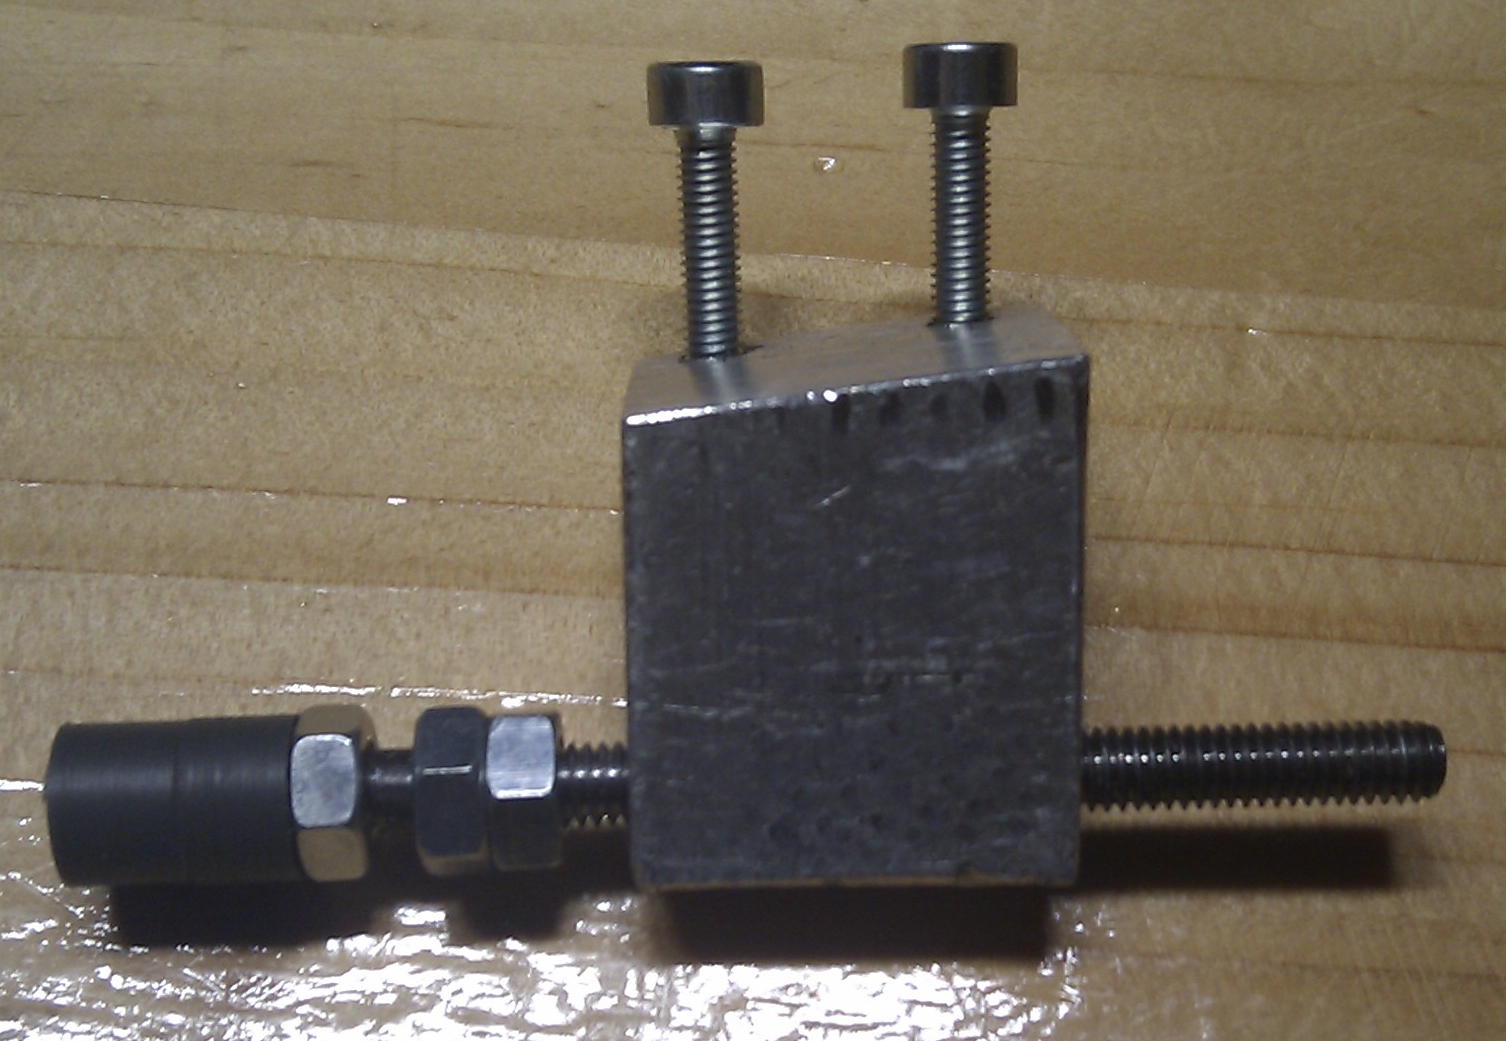
\includegraphics[width = \textwidth]{pics/raw/encoder_mount.png}
  \end{center}
    \column{0.5\textwidth}
  \begin{center}
  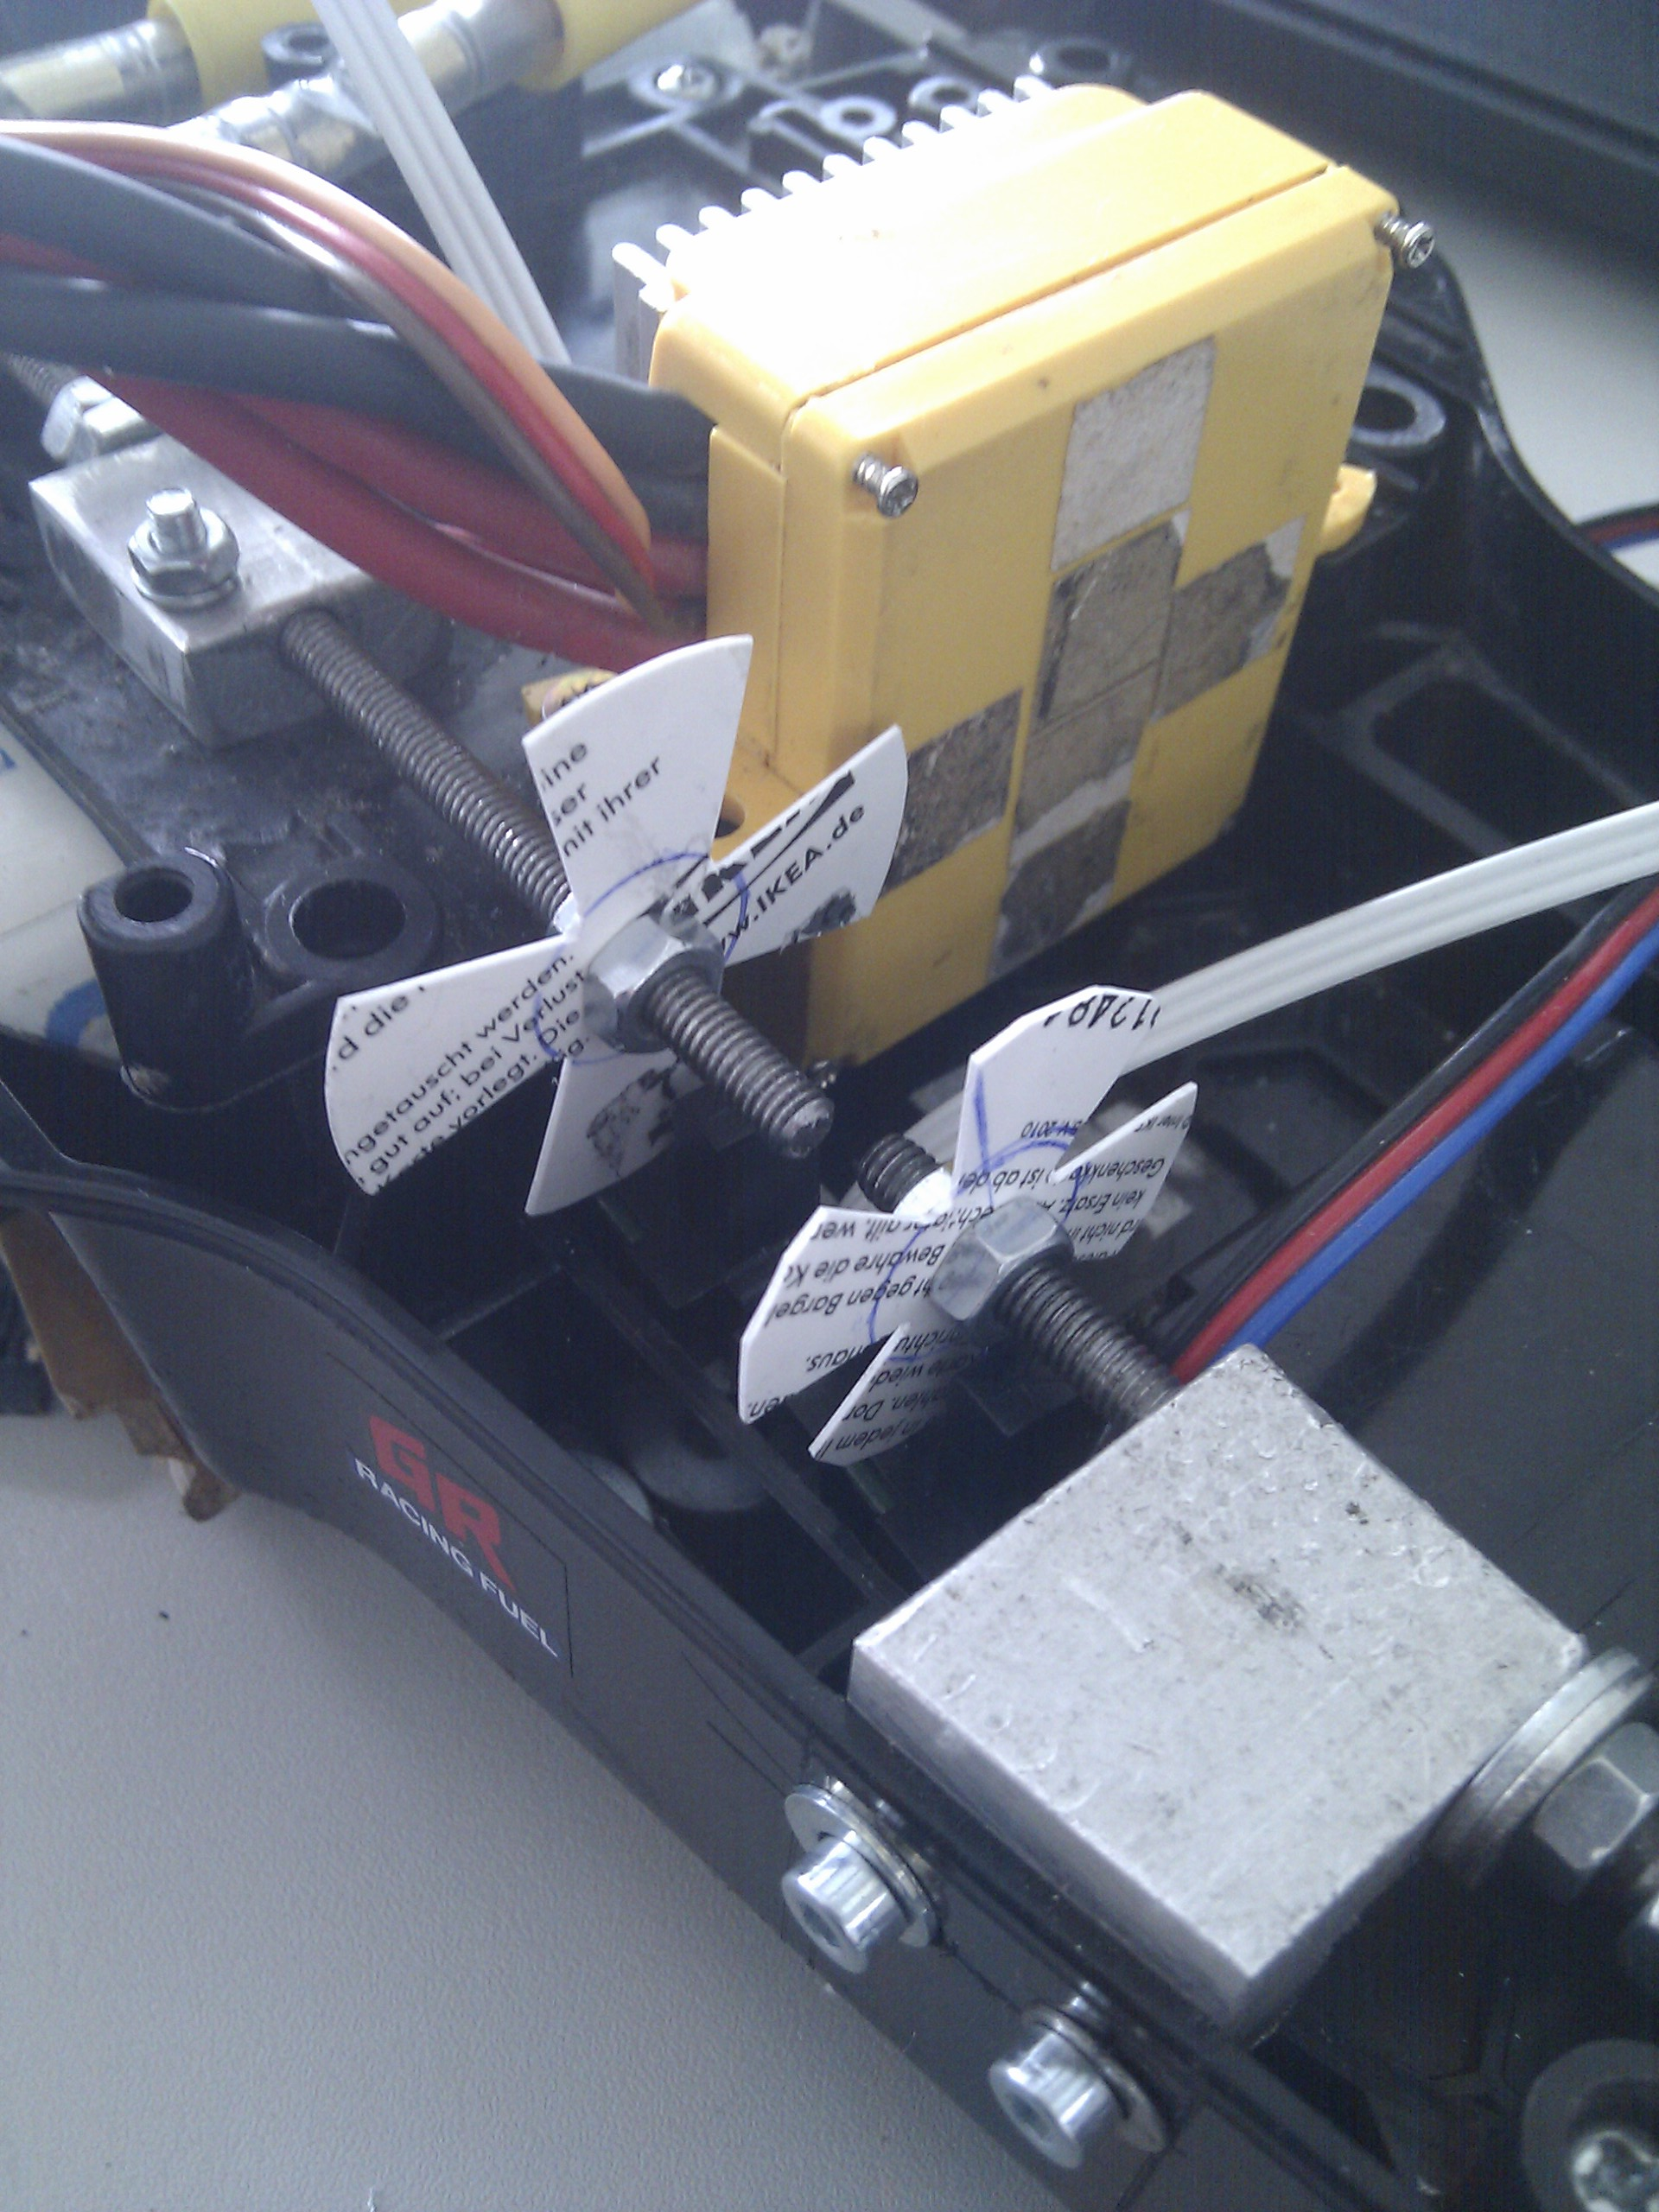
\includegraphics[width = \textwidth]{pics/raw/encoders_scheiben.jpg}
  \end{center}
  \end{columns}
\end{frame}

\section{Electronics}
\subsection{Encoder - PCB}
\begin{frame}
  \begin{columns}
    \column{0.5\textwidth}
      \begin{center}
      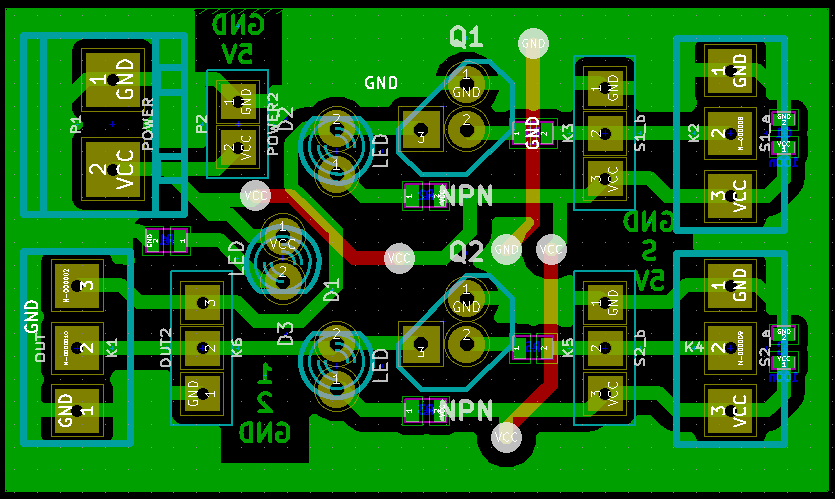
\includegraphics[width = 1.0\textwidth]{pics/raw/sensor.png}\\
      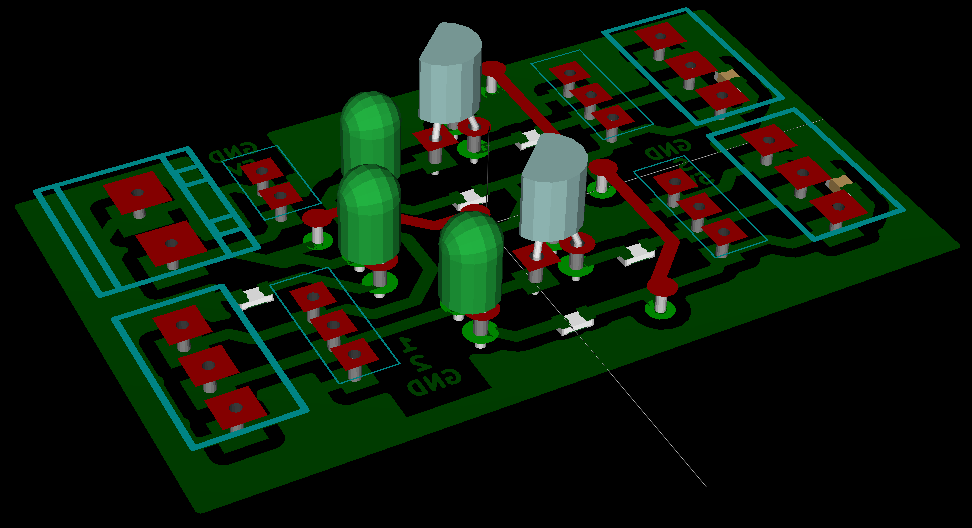
\includegraphics[width = 1.0\textwidth]{pics/raw/sensor2.png}
      \end{center}
    \column{0.5\textwidth}
      \begin{itemize}
        \item Connect 2 sensors
        \item Decouple sensors from FPGA
        \item Provide 5V digital output
        \item Signal LEDs for debugging
      \end{itemize}
  \end{columns}
\end{frame}

\section{Detecting obstacles}
\subsection{Home built low cost LASER!! scanner}
\begin{frame}
\begin{alertblock}{Problem}
\begin{itemize}
  \item We have to detect objects in front of us
  \item Commercial 3D scanners are too expensive
  \item Kinect ist too unreliable, slow and hard to interface (USB)
\end{itemize}
\end{alertblock}
\begin{exampleblock}{Solution}
\begin{itemize}
  \item Build our own LASER SCANNER
  \item (Yes LASER like in the movies)
  \item Low cost: 12 EUR + Webcam
  \item[...] not sure it will work
\end{itemize}
\end{exampleblock}
\end{frame}
\begin{frame}
  \begin{center}
  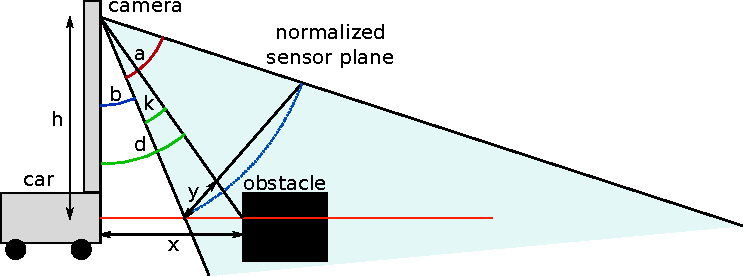
\includegraphics[width = 0.9\textwidth]{pics/laser.pdf}
  \end{center}
$$y\approx \frac{k}{a} \hspace{1cm} k = d - b$$
$$d = arctan\left( \frac{x}{h} \right)$$
$$\Rightarrow y = \frac{arctan \left( \frac{x}{h} \right) - b }{a}$$
\end{frame}

\begin{frame}
\frametitle{Dynamic resolution}
  \begin{center}
  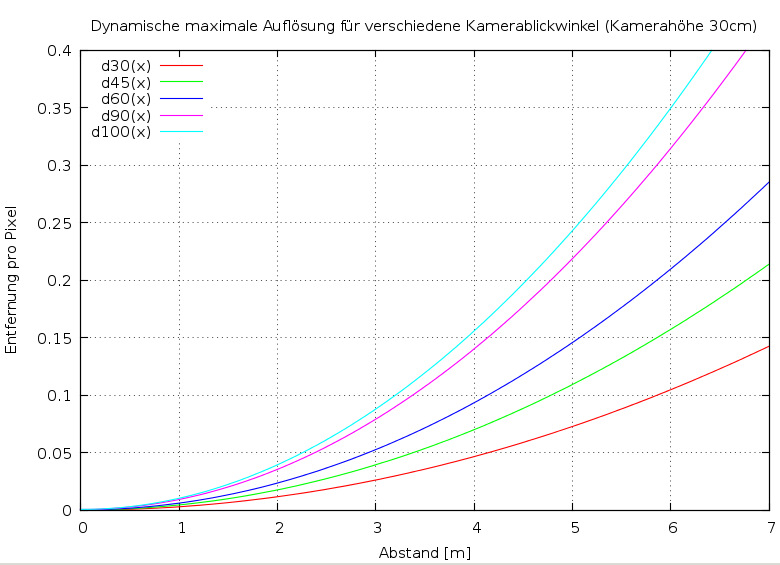
\includegraphics[width = 0.7\textwidth]{pics/raw/scanner_aufloesung.png}
  \end{center}
\end{frame}

\begin{frame}
\frametitle{Proof of concept}
  \begin{columns}
    \column{0.4\textwidth}
  \begin{center}
  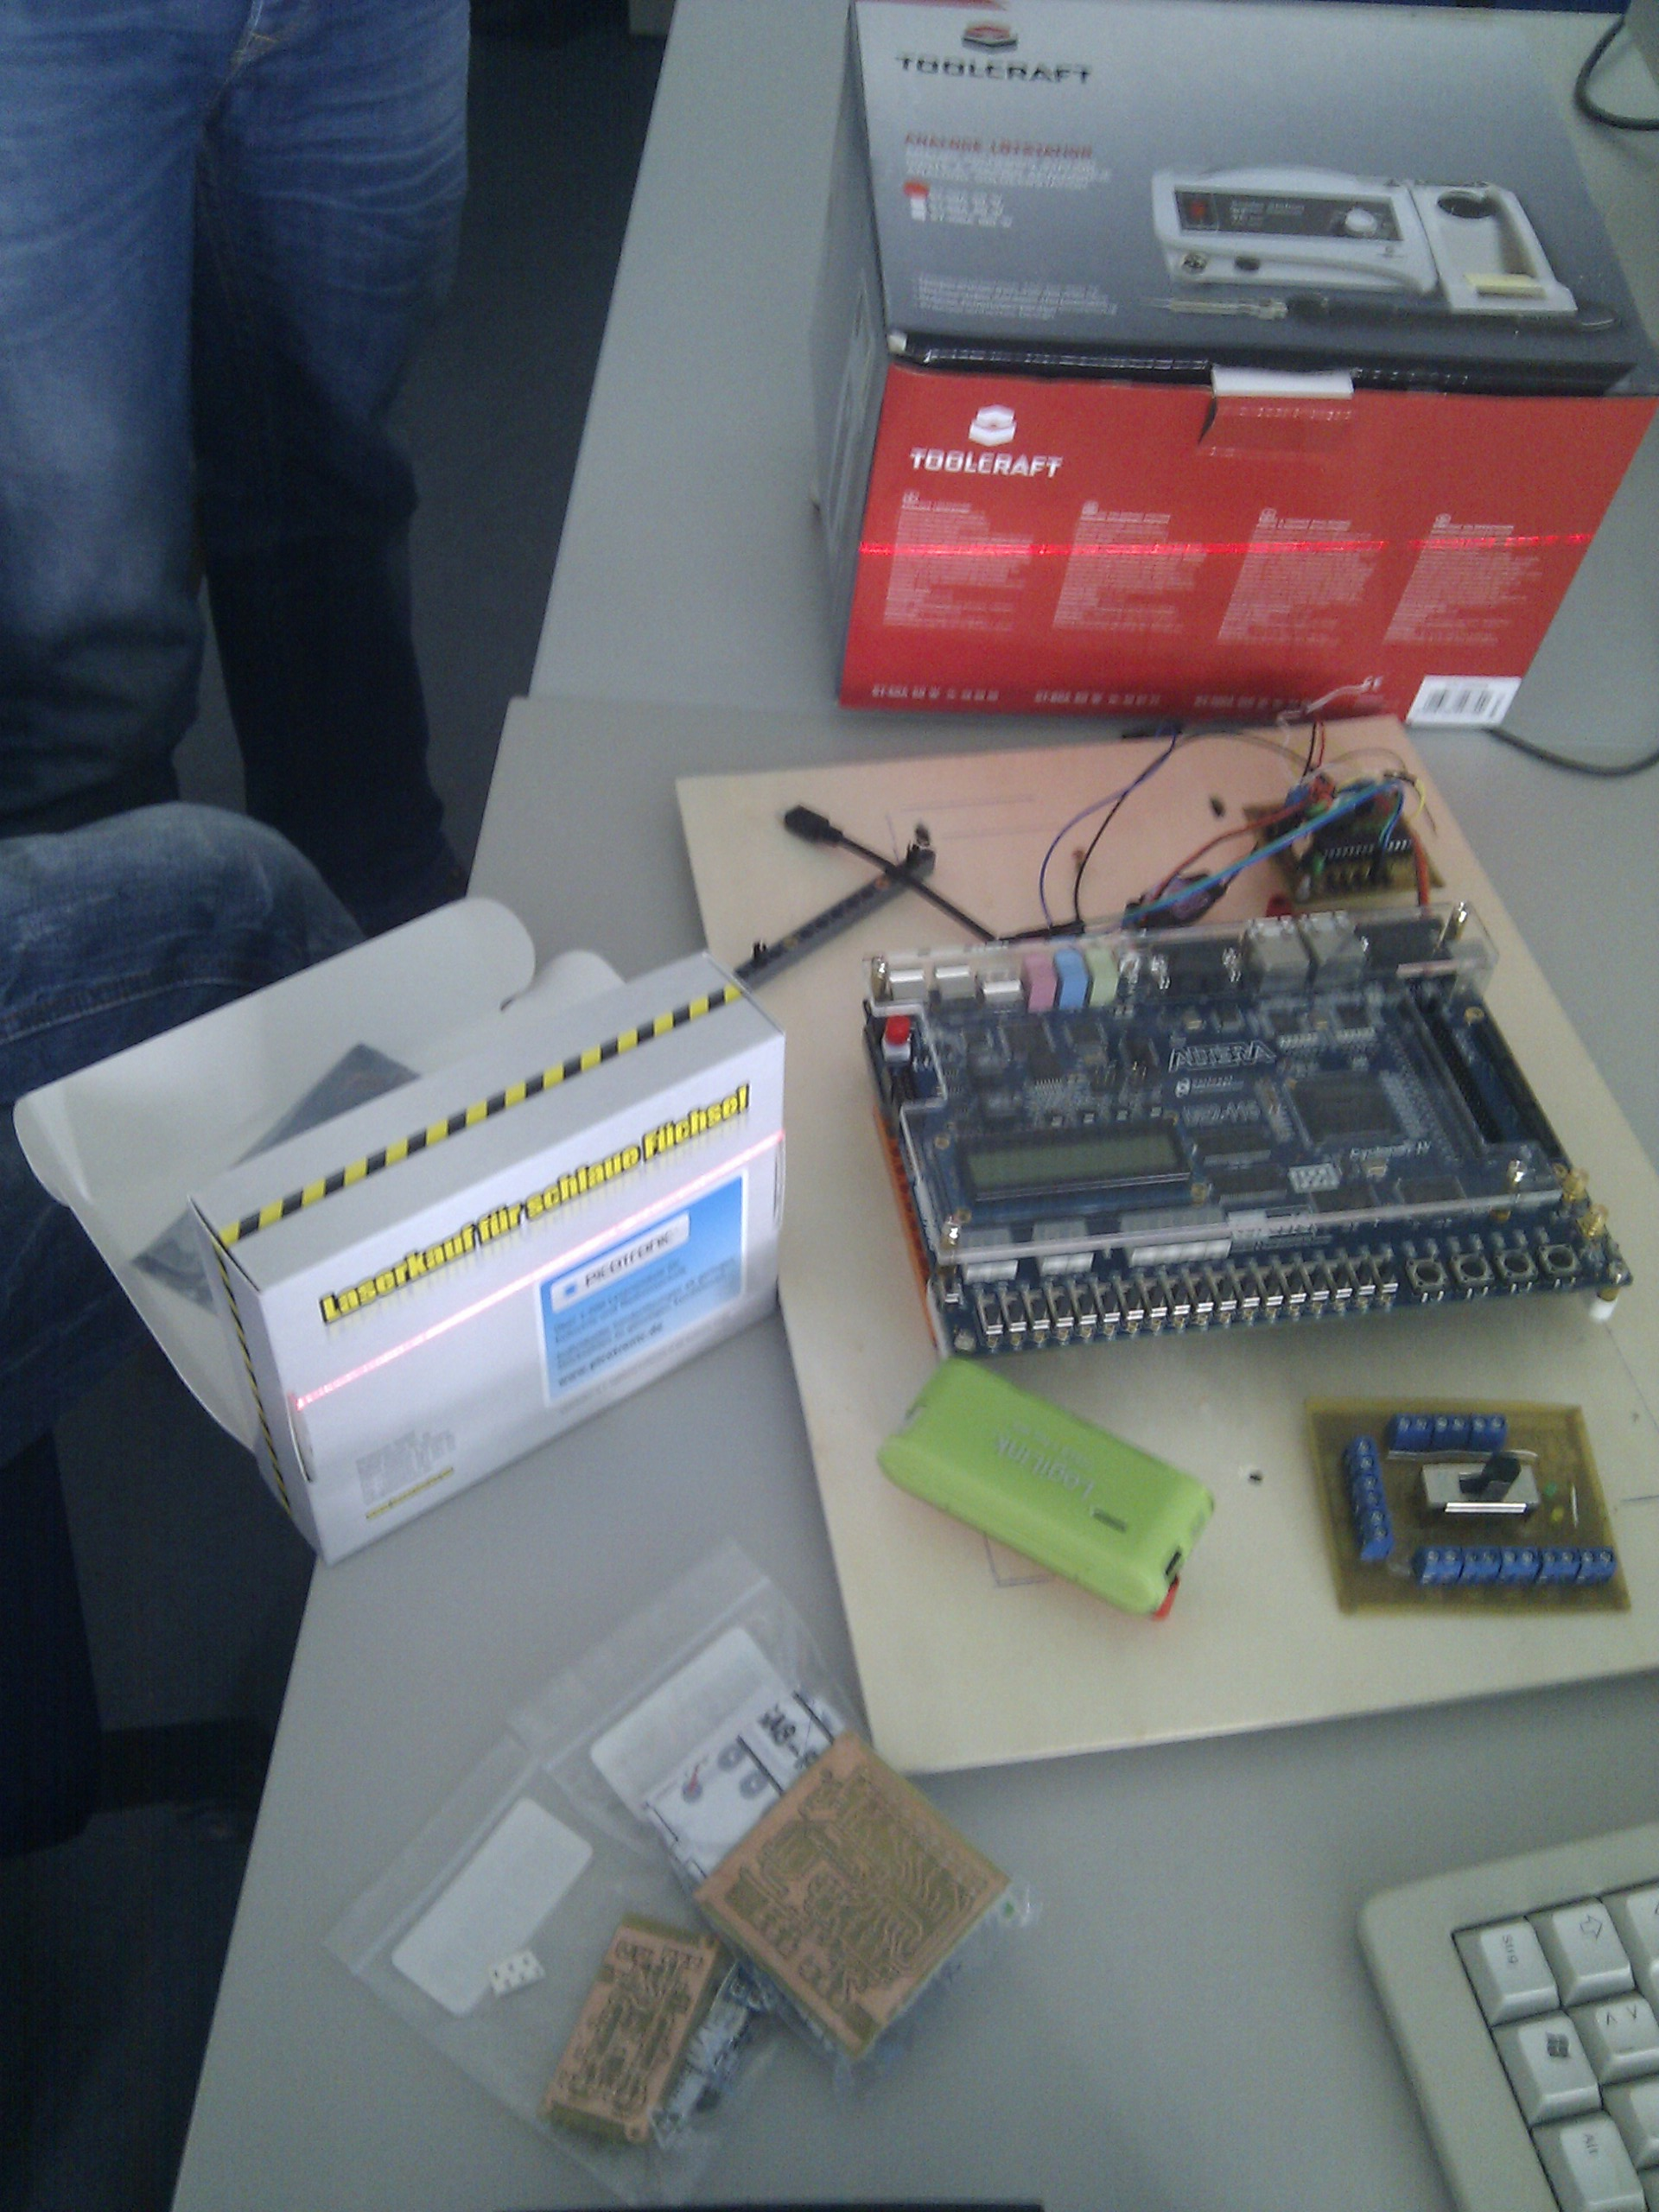
\includegraphics[width = \textwidth]{pics/raw/laser_test.jpg}
  \end{center}
    \column{0.6\textwidth}
  \begin{center}
  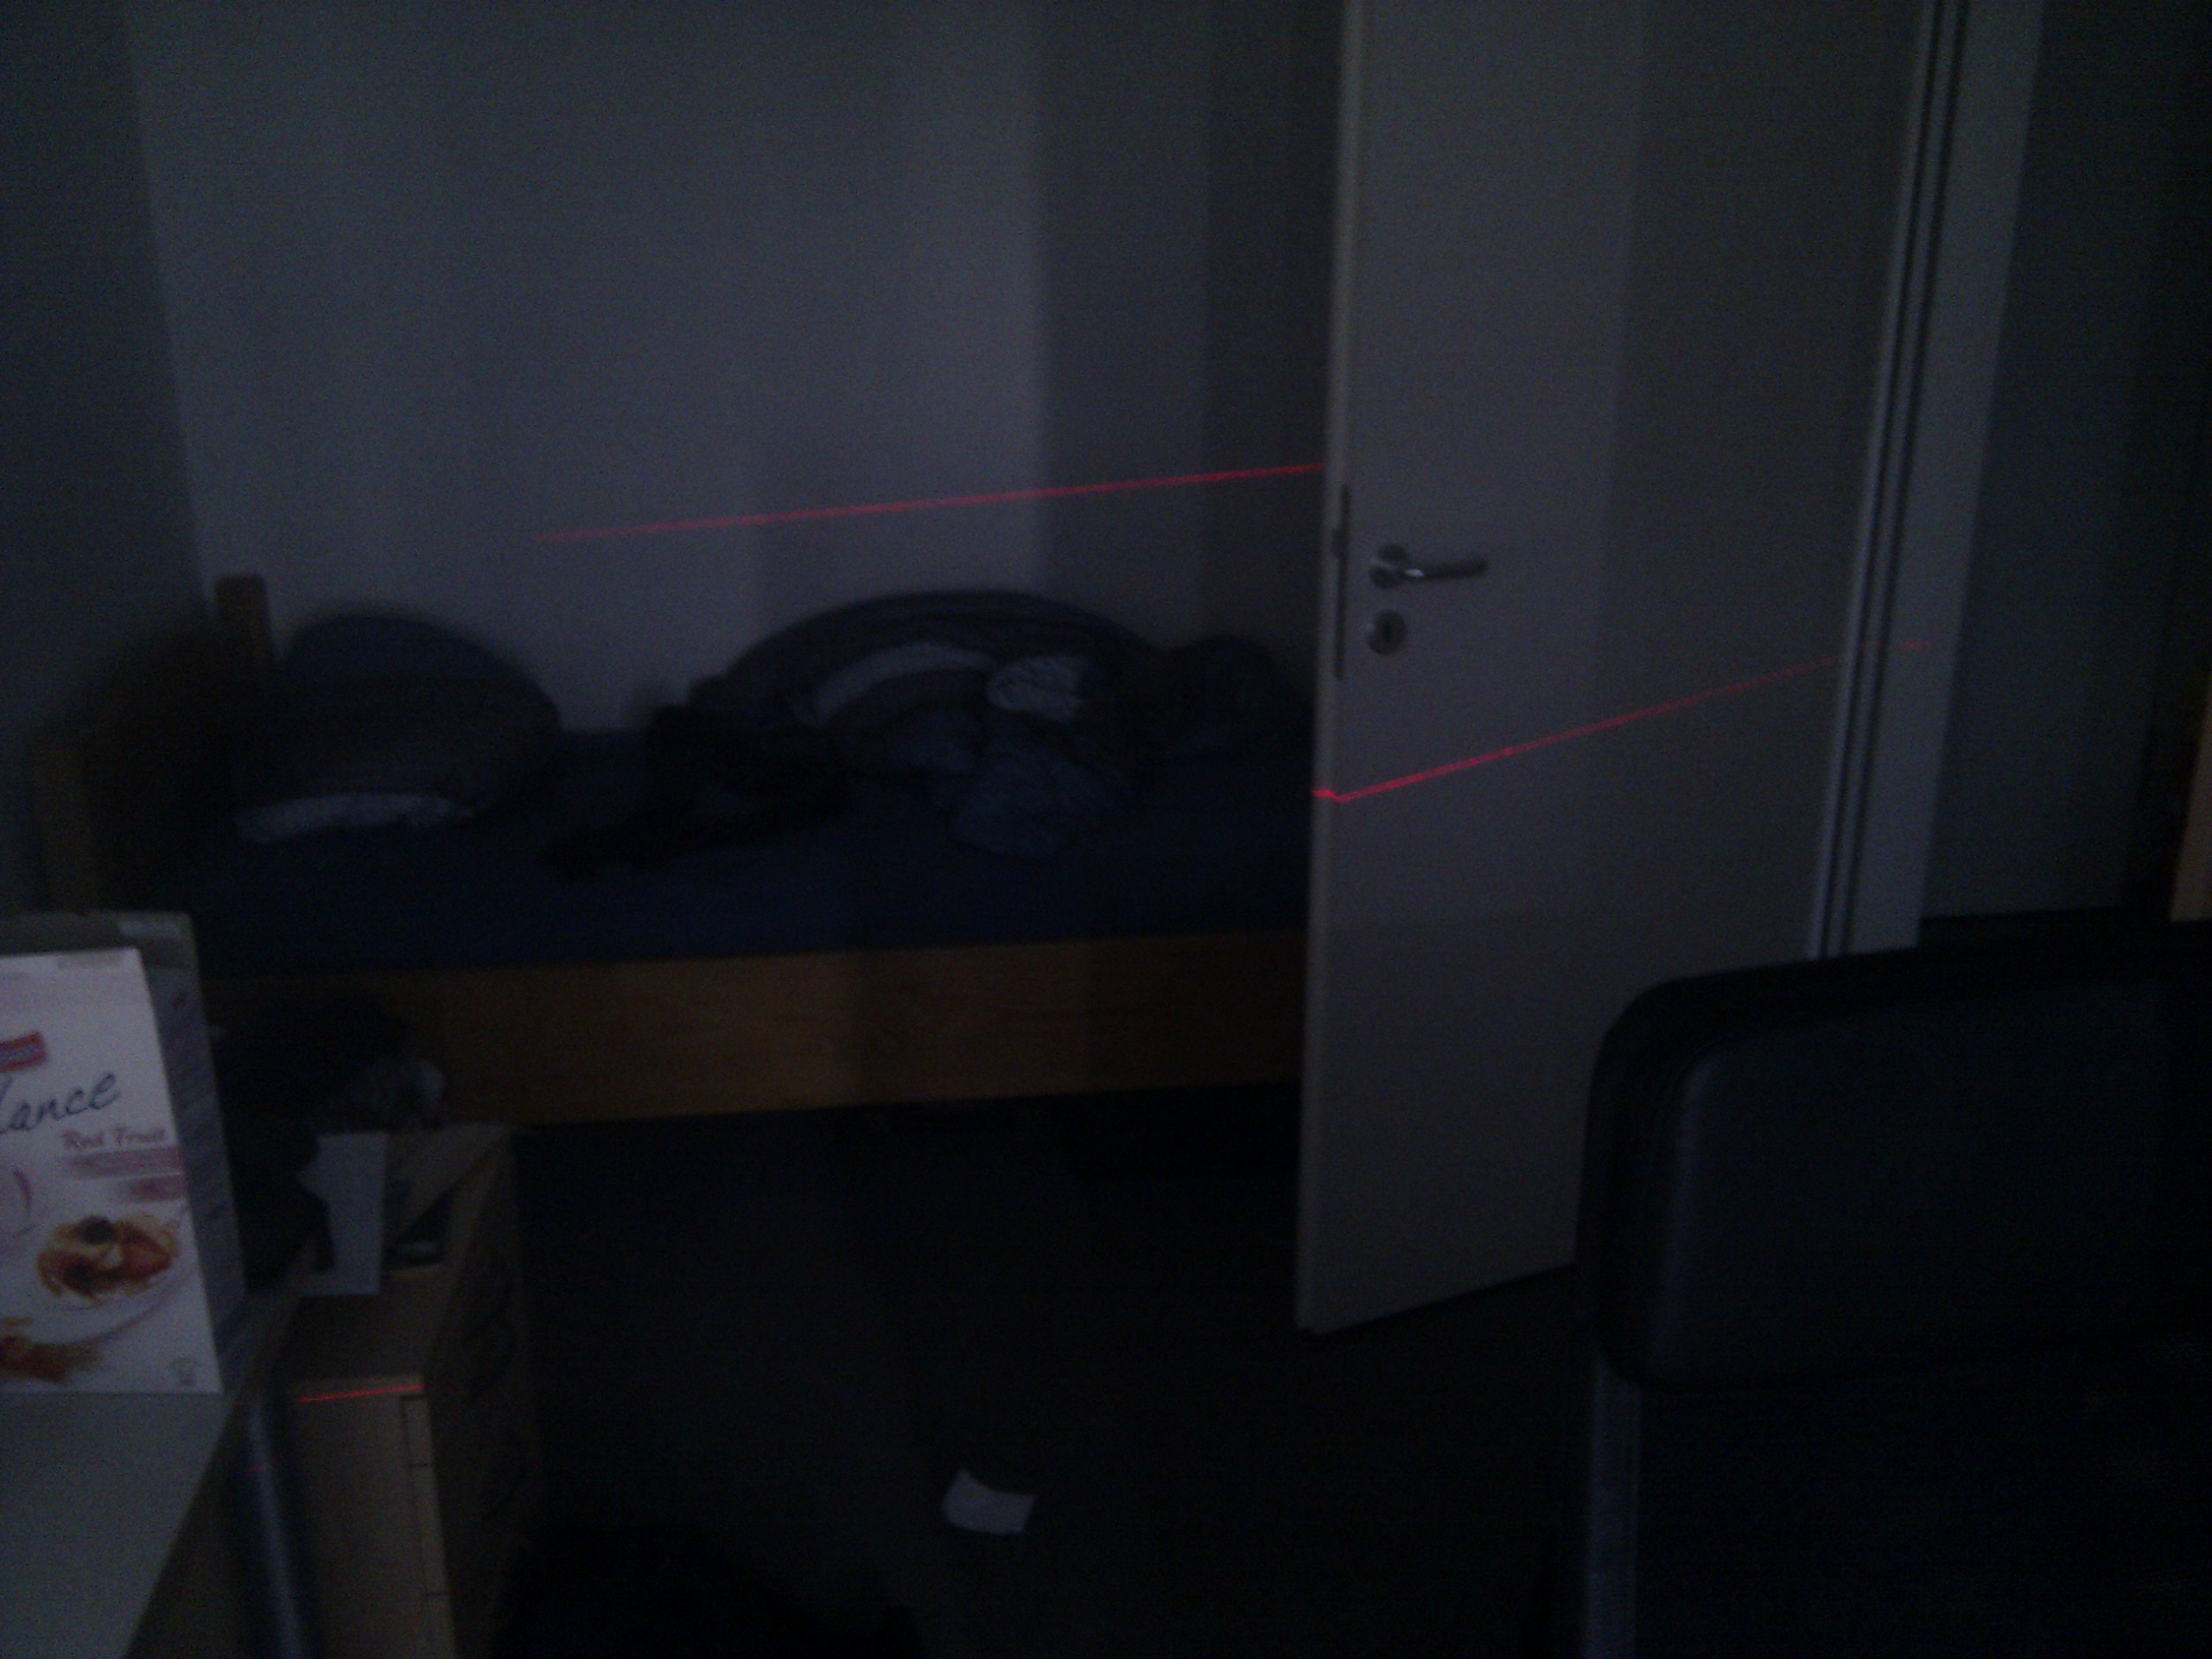
\includegraphics[width = \textwidth]{pics/raw/laser_weak.png}
  \end{center}
  \end{columns}
\end{frame}

\begin{frame}
\frametitle{Mounting the laser}
  \begin{center}
  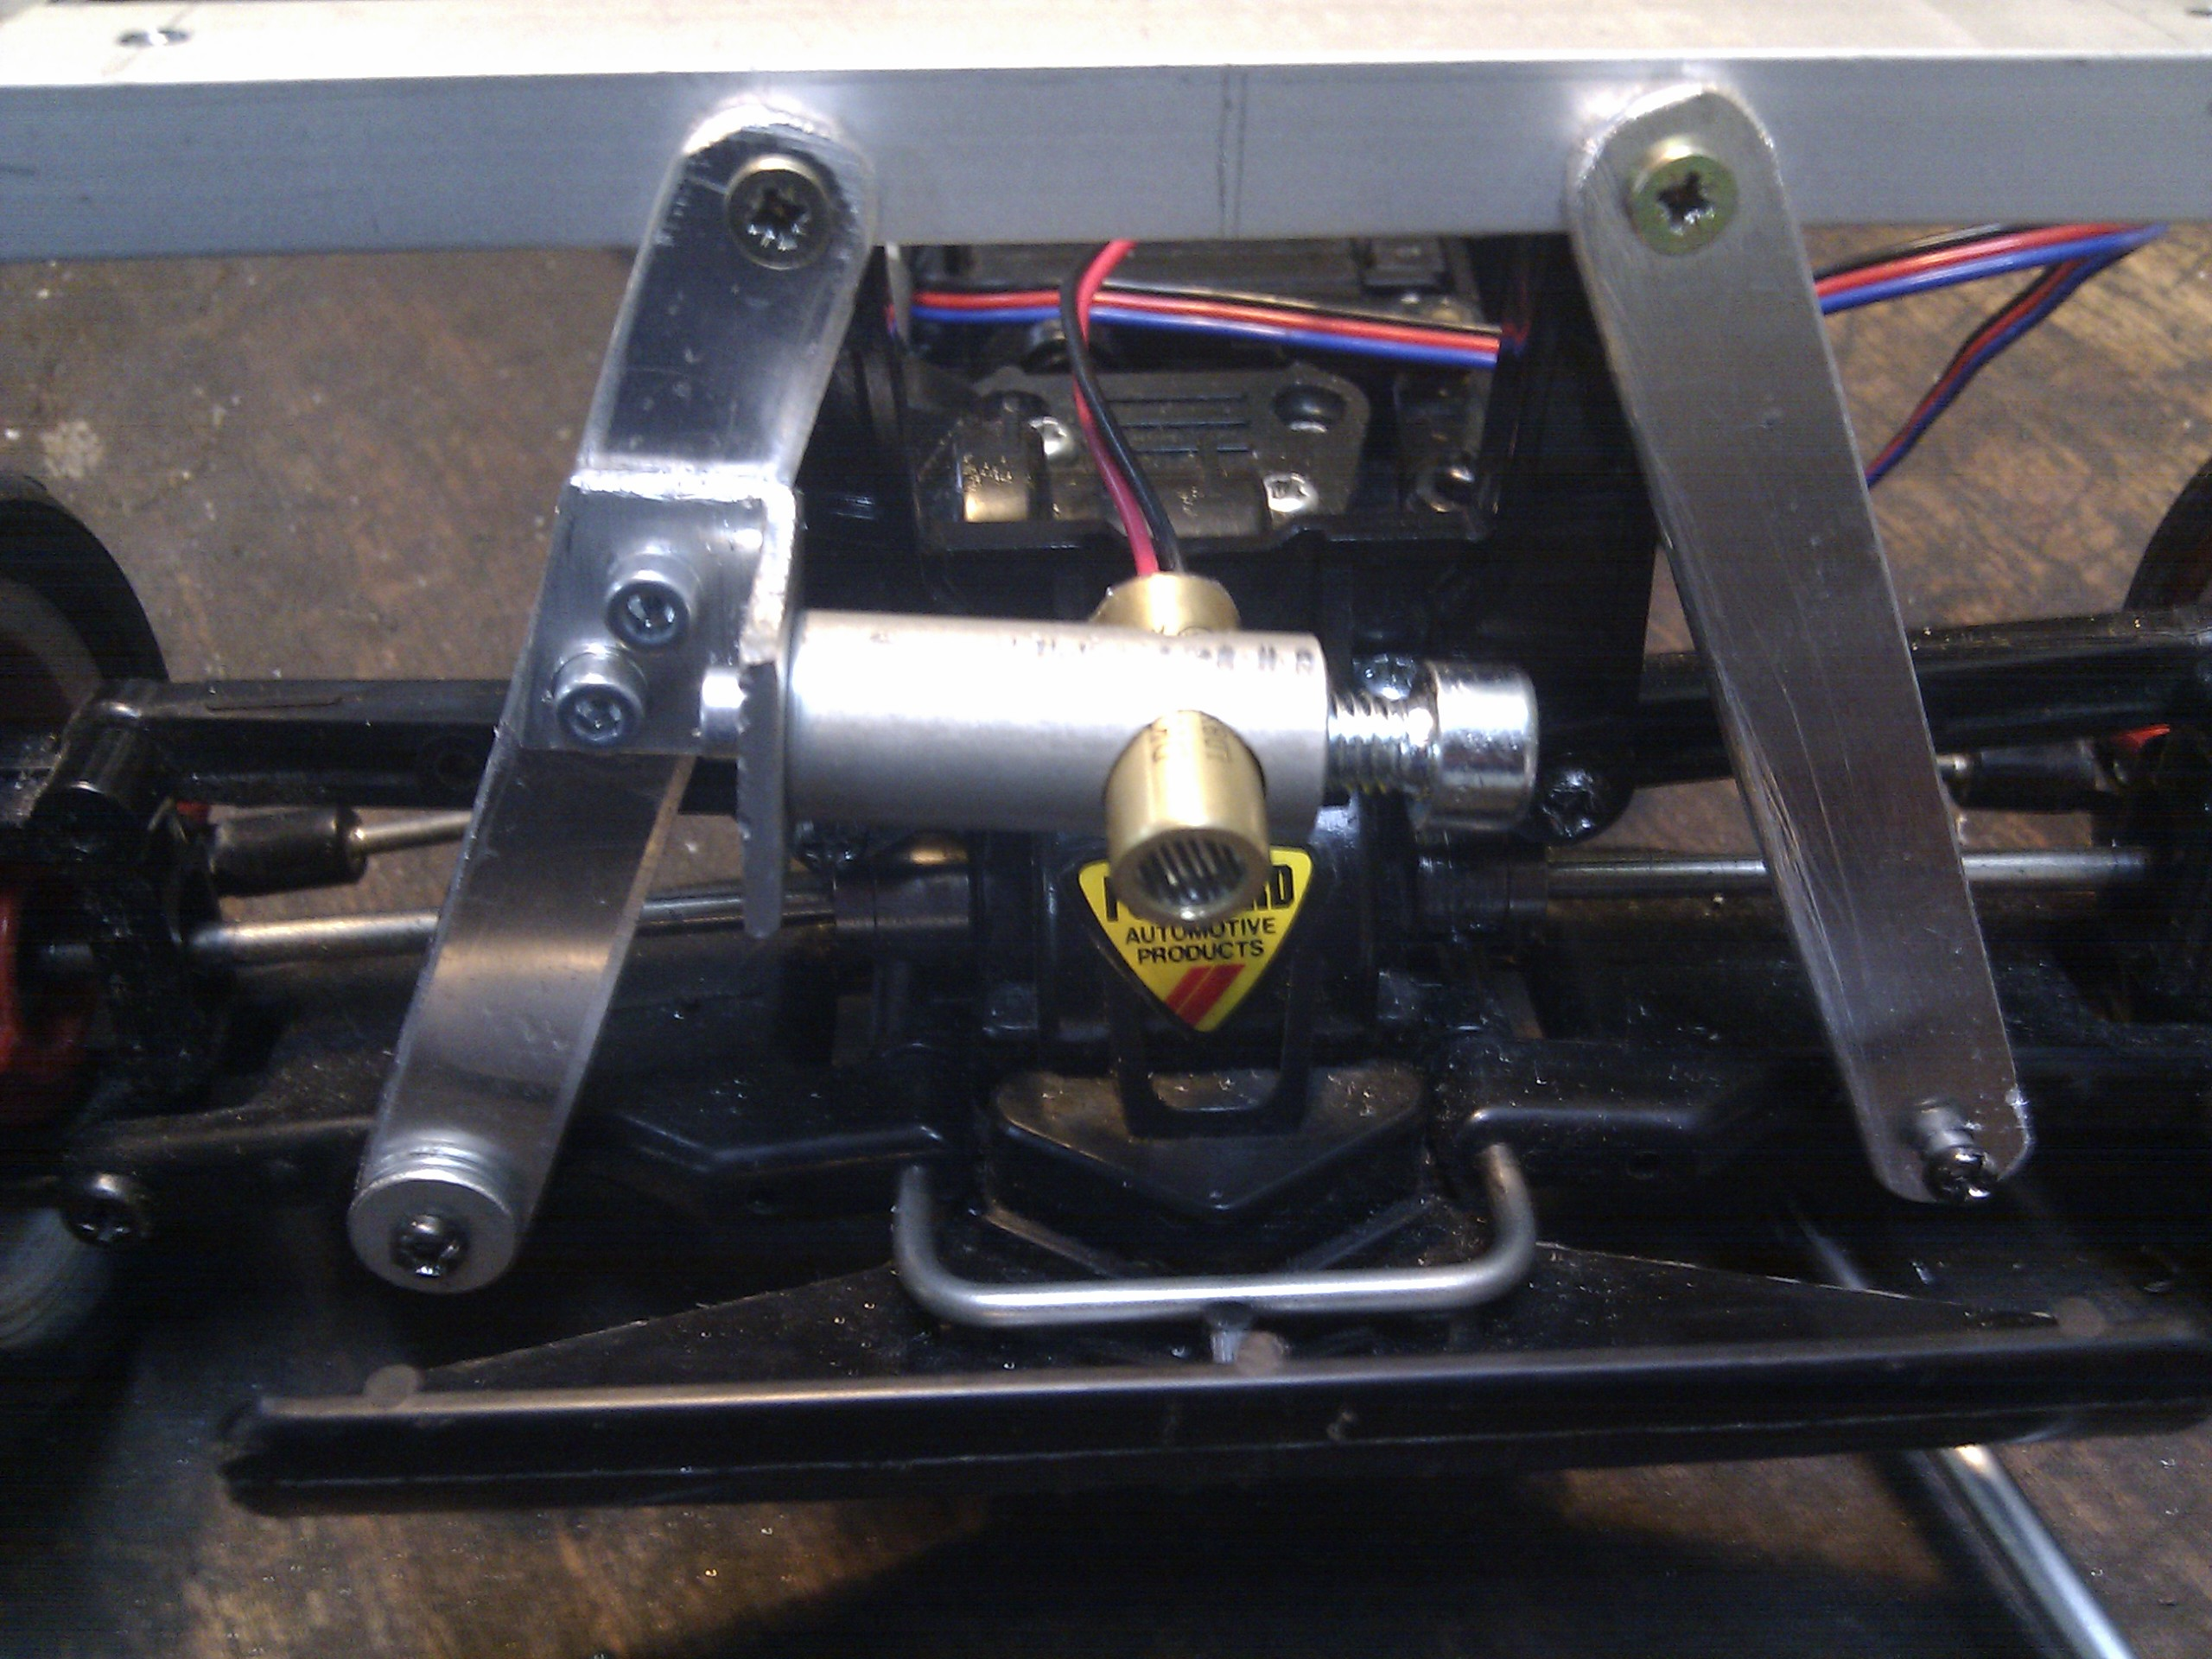
\includegraphics[width = 0.9\textwidth]{pics/raw/laser_mount2.jpg}
  \end{center}
\end{frame}

\section{Complete System}
\subsection{Idea}
\begin{frame}
\frametitle{FPGA + RaspPi + custom PCB + Sensors}
  \begin{center}
  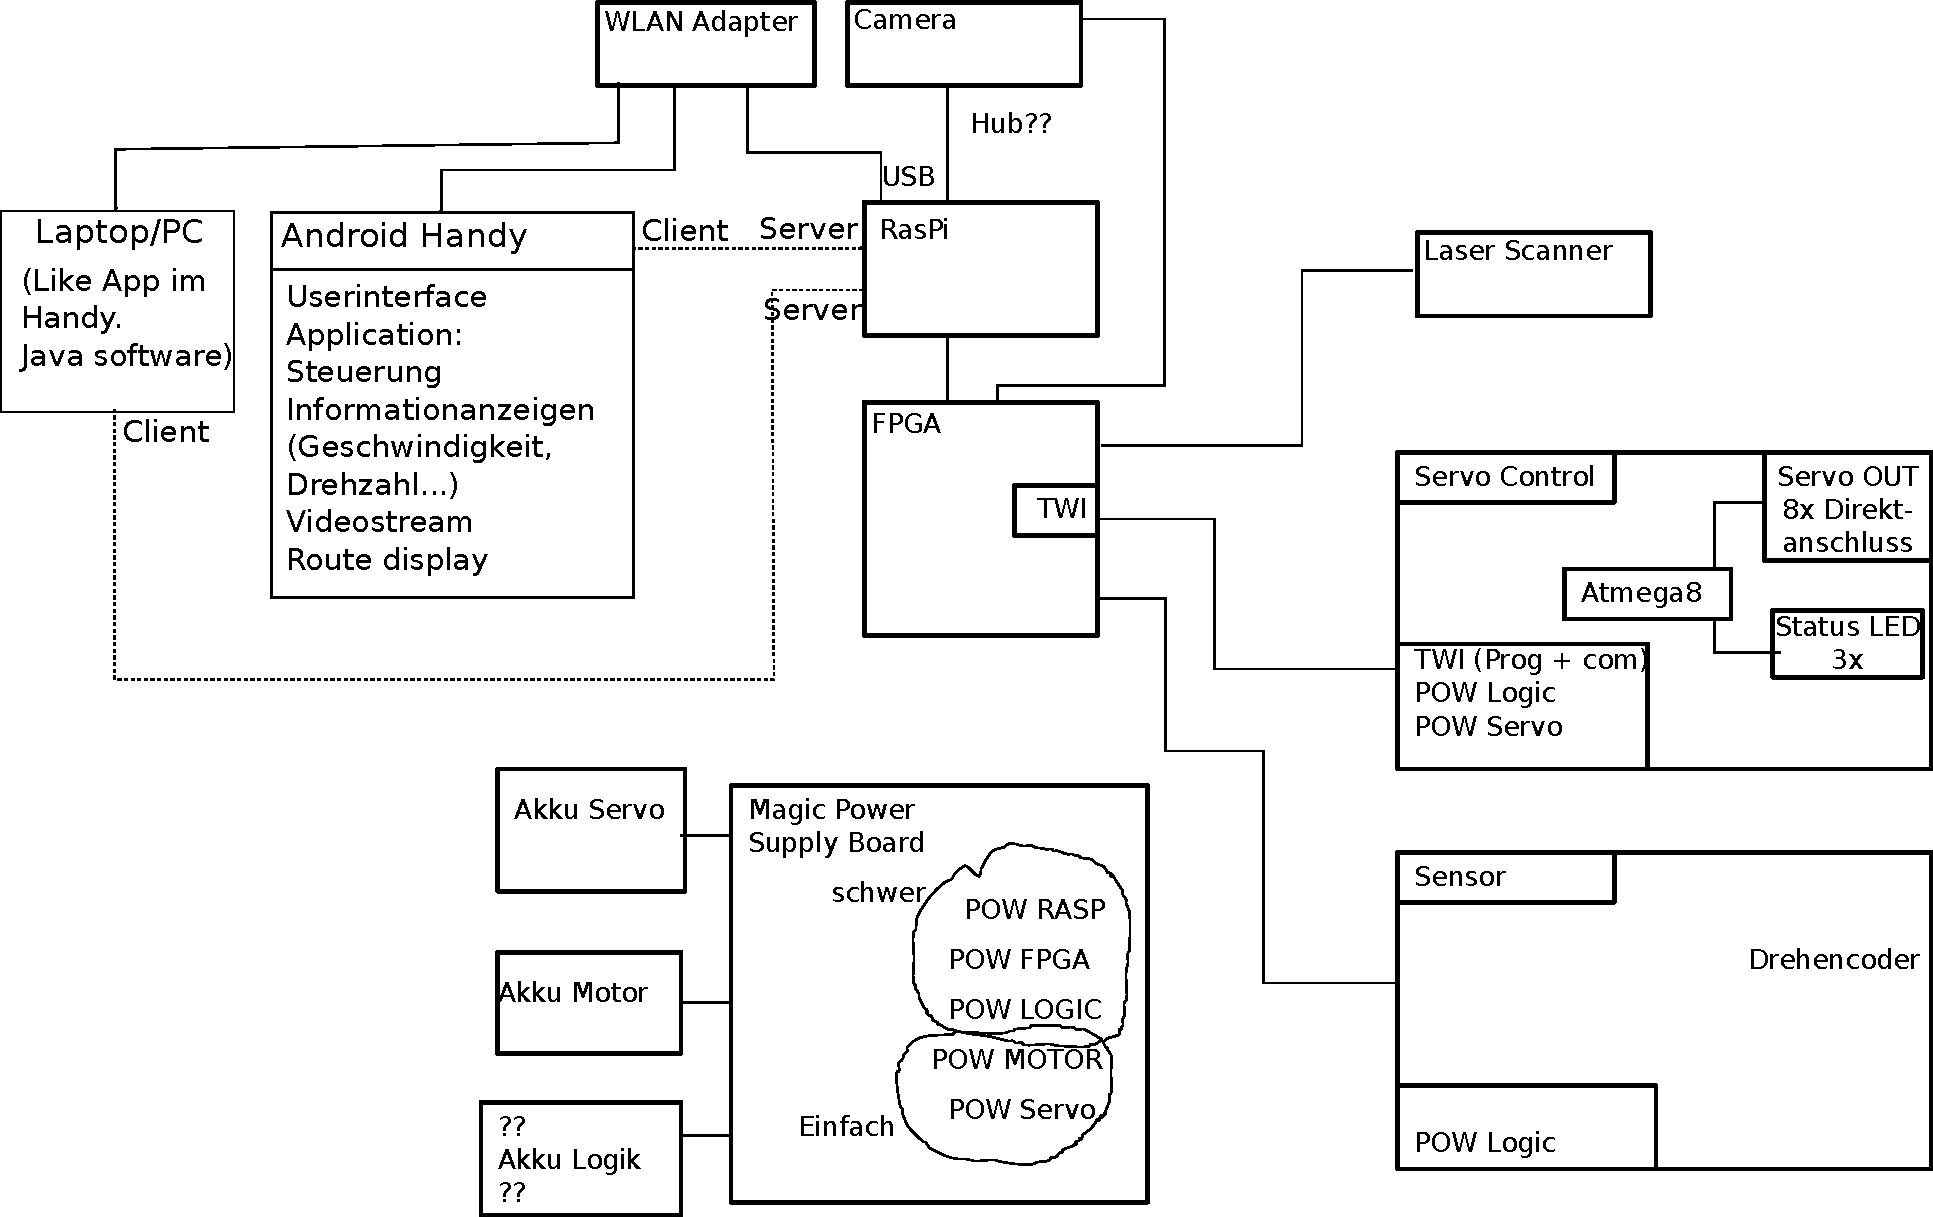
\includegraphics[width = 0.9\textwidth]{pics/design.pdf}
  \end{center}
\end{frame}


\section{User Interfaces}
\subsection{Cellphone}
\begin{frame}
\frametitle{Android Setting Page}
  \begin{center}
   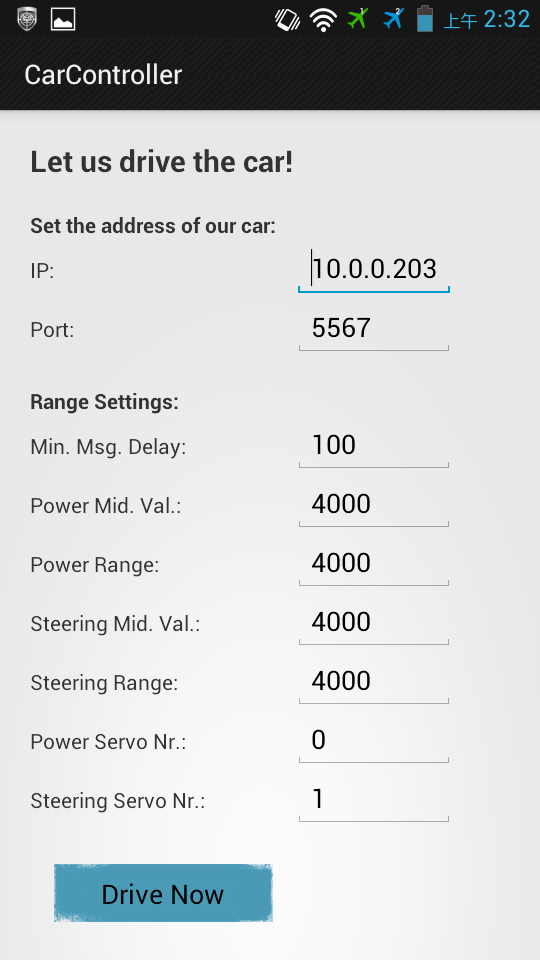
\includegraphics[height = 0.8\textheight]{pics/android_settings.png}  
  \end{center}
\end{frame}
\begin{frame}
\frametitle{Android Control Page}
  \begin{center}
   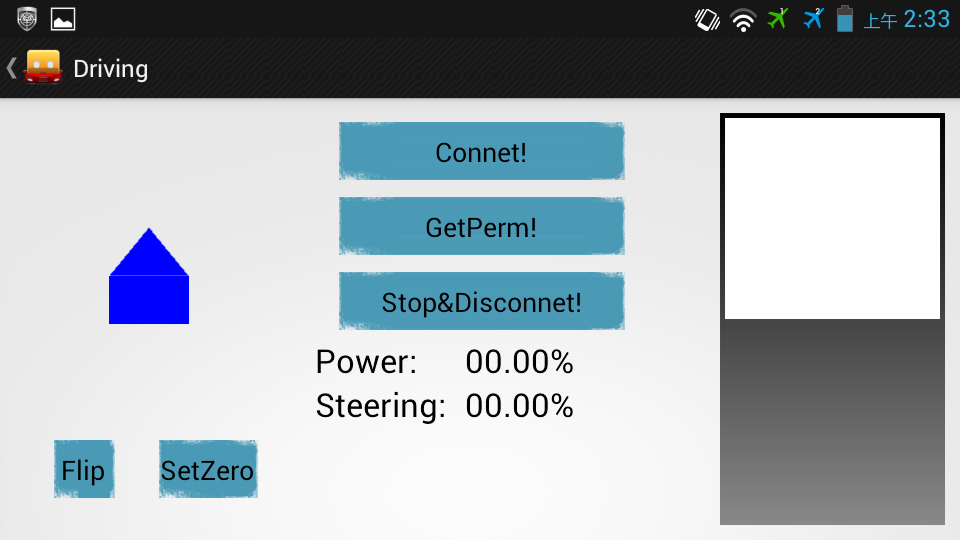
\includegraphics[width = 0.55\textwidth]{pics/android_control.png}\\  
   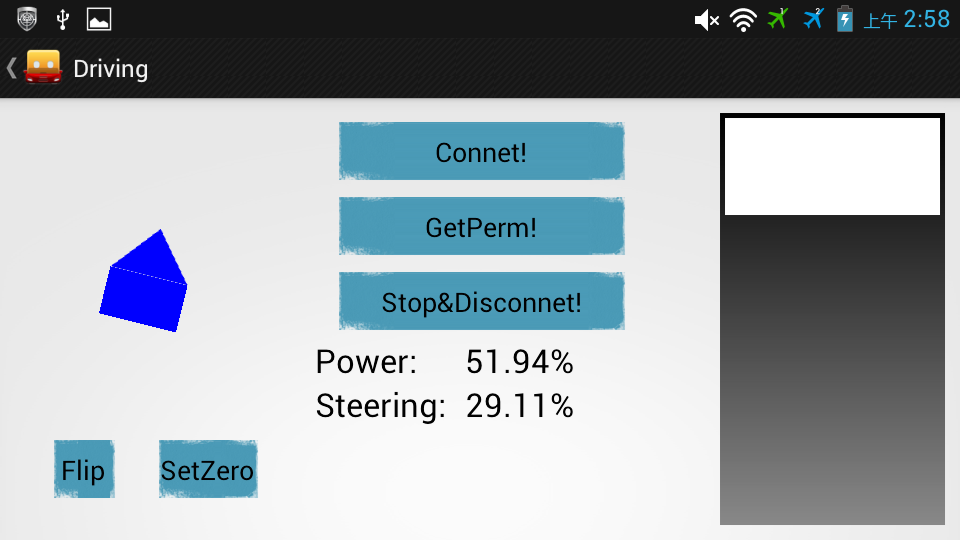
\includegraphics[width = 0.55\textwidth]{pics/android_controlling.png}     
  \end{center}
\end{frame}

\subsection{Console Controller}
\begin{frame}
\frametitle{WII}
  \begin{center}
  \end{center}
\end{frame}


\section{Simulation}
\subsection{Problem}
\begin{frame}
\begin{alertblock}{Problem}
\begin{itemize}
  \item Hardware difficult to test
  \item Not everyone has access to the car all the time
  \item Car has limited battery power
  \item Bug $\rightarrow$ Is it a software or a hardware problem?
\end{itemize}
\end{alertblock}
\begin{exampleblock}{Solution}
\begin{itemize}
  \item Simulate car in real time
  \item And sensors
  \item Provide same interface as real car
  \item Connect real hardware to simulation
\end{itemize}
\end{exampleblock}
\end{frame}
\section{We are working on...}
\subsection{Test setup}
\begin{frame}
Testing GUIs, TCP/UDP/IP Protocols, Hardware
  \begin{center}
  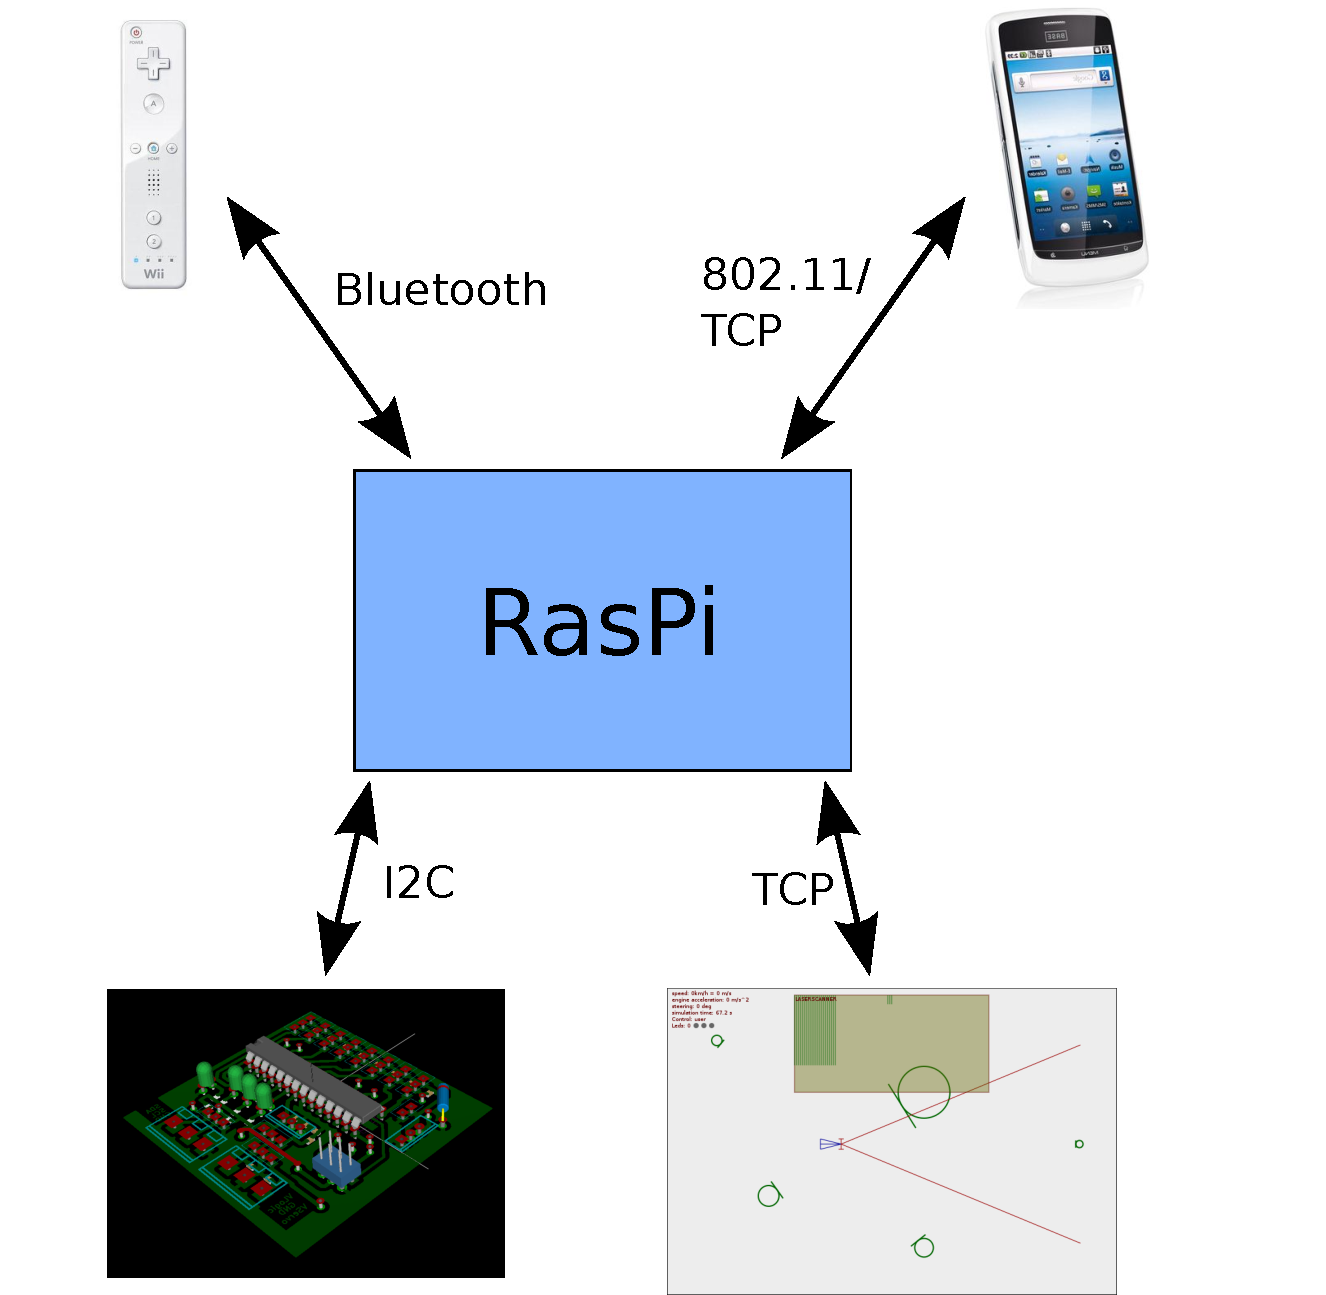
\includegraphics[width = 0.7\textwidth]{pics/raw/software2.pdf}
  \end{center}
\end{frame}
\begin{frame}
\frametitle{Demo}
  \begin{center}
  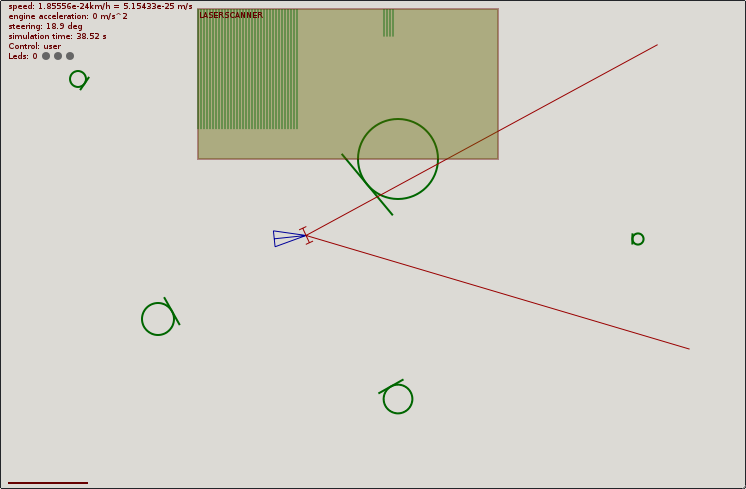
\includegraphics[width = 0.8\textwidth]{pics/raw/sim.png}
  \end{center}
\end{frame}
\subsection{FPGA}
\begin{frame}
\frametitle{Implementing I2C}
\end{frame}

\section{Goals}
\begin{frame}
\frametitle{Future steps}
\begin{exampleblock}{Plan}
\begin{itemize}
\item Assisted remote controlled car
\item Flexible heterogenous user interfaces (Android, Laptop, Wii, PS Controller)
\item Traction control
\item Obstacle avoidance via laserscanner
\item Drive in convoy (second camera)
\end{itemize}
\end{exampleblock}
\begin{alertblock}{Problems}
\begin{itemize}
\item Laser is very weak and hence hard to detect
\item Communication via Wifi is unstable and short ranged
\item Time
\end{itemize}

\end{alertblock}
\end{frame}


\end{document}
